\documentclass[twoside]{book}

% Packages required by doxygen
\usepackage{fixltx2e}
\usepackage{calc}
\usepackage{doxygen}
\usepackage[export]{adjustbox} % also loads graphicx
\usepackage{graphicx}
\usepackage[utf8]{inputenc}
\usepackage{makeidx}
\usepackage{multicol}
\usepackage{multirow}
\PassOptionsToPackage{warn}{textcomp}
\usepackage{textcomp}
\usepackage[nointegrals]{wasysym}
\usepackage[table]{xcolor}

% Font selection
\usepackage[T1]{fontenc}
\usepackage[scaled=.90]{helvet}
\usepackage{courier}
\usepackage{amssymb}
\usepackage{sectsty}
\renewcommand{\familydefault}{\sfdefault}
\allsectionsfont{%
  \fontseries{bc}\selectfont%
  \color{darkgray}%
}
\renewcommand{\DoxyLabelFont}{%
  \fontseries{bc}\selectfont%
  \color{darkgray}%
}
\newcommand{\+}{\discretionary{\mbox{\scriptsize$\hookleftarrow$}}{}{}}

% Page & text layout
\usepackage{geometry}
\geometry{%
  a4paper,%
  top=2.5cm,%
  bottom=2.5cm,%
  left=2.5cm,%
  right=2.5cm%
}
\tolerance=750
\hfuzz=15pt
\hbadness=750
\setlength{\emergencystretch}{15pt}
\setlength{\parindent}{0cm}
\setlength{\parskip}{3ex plus 2ex minus 2ex}
\makeatletter
\renewcommand{\paragraph}{%
  \@startsection{paragraph}{4}{0ex}{-1.0ex}{1.0ex}{%
    \normalfont\normalsize\bfseries\SS@parafont%
  }%
}
\renewcommand{\subparagraph}{%
  \@startsection{subparagraph}{5}{0ex}{-1.0ex}{1.0ex}{%
    \normalfont\normalsize\bfseries\SS@subparafont%
  }%
}
\makeatother

% Headers & footers
\usepackage{fancyhdr}
\pagestyle{fancyplain}
\fancyhead[LE]{\fancyplain{}{\bfseries\thepage}}
\fancyhead[CE]{\fancyplain{}{}}
\fancyhead[RE]{\fancyplain{}{\bfseries\leftmark}}
\fancyhead[LO]{\fancyplain{}{\bfseries\rightmark}}
\fancyhead[CO]{\fancyplain{}{}}
\fancyhead[RO]{\fancyplain{}{\bfseries\thepage}}
\fancyfoot[LE]{\fancyplain{}{}}
\fancyfoot[CE]{\fancyplain{}{}}
\fancyfoot[RE]{\fancyplain{}{\bfseries\scriptsize Generated by Doxygen }}
\fancyfoot[LO]{\fancyplain{}{\bfseries\scriptsize Generated by Doxygen }}
\fancyfoot[CO]{\fancyplain{}{}}
\fancyfoot[RO]{\fancyplain{}{}}
\renewcommand{\footrulewidth}{0.4pt}
\renewcommand{\chaptermark}[1]{%
  \markboth{#1}{}%
}
\renewcommand{\sectionmark}[1]{%
  \markright{\thesection\ #1}%
}

% Indices & bibliography
\usepackage{natbib}
\usepackage[titles]{tocloft}
\setcounter{tocdepth}{3}
\setcounter{secnumdepth}{5}
\makeindex

% Hyperlinks (required, but should be loaded last)
\usepackage{ifpdf}
\ifpdf
  \usepackage[pdftex,pagebackref=true]{hyperref}
\else
  \usepackage[ps2pdf,pagebackref=true]{hyperref}
\fi
\hypersetup{%
  colorlinks=true,%
  linkcolor=blue,%
  citecolor=blue,%
  unicode%
}

% Custom commands
\newcommand{\clearemptydoublepage}{%
  \newpage{\pagestyle{empty}\cleardoublepage}%
}

\usepackage{caption}
\captionsetup{labelsep=space,justification=centering,font={bf},singlelinecheck=off,skip=4pt,position=top}

%===== C O N T E N T S =====

\begin{document}

% Titlepage & ToC
\hypersetup{pageanchor=false,
             bookmarksnumbered=true,
             pdfencoding=unicode
            }
\pagenumbering{alph}
\begin{titlepage}
\vspace*{7cm}
\begin{center}%
{\Large N\+ES Snake }\\
\vspace*{1cm}
{\large Generated by Doxygen 1.8.12}\\
\end{center}
\end{titlepage}
\clearemptydoublepage
\pagenumbering{roman}
\tableofcontents
\clearemptydoublepage
\pagenumbering{arabic}
\hypersetup{pageanchor=true}

%--- Begin generated contents ---
\chapter{R\+E\+A\+D\+ME}
\label{md__c_1__users__administrator__documents__git_hub__n_e_s-_snake__r_e_a_d_m_e}
\hypertarget{md__c_1__users__administrator__documents__git_hub__n_e_s-_snake__r_e_a_d_m_e}{}
N\+ES Snake This project is my first attempt to write a simple N\+ES Snake game using Shiru´s N\+E\+S\+Library, based on the C\+C65 project. You can find out more about Shiru´s N\+E\+S\+Library here\+: \href{http://shiru.untergrund.net/articles/programming_nes_games_in_c.htm}{\tt http\+://shiru.\+untergrund.\+net/articles/programming\+\_\+nes\+\_\+games\+\_\+in\+\_\+c.\+htm} Also, if you are interested in the general C\+C65 project, you can find it here\+: \href{http://www.cc65.org/}{\tt http\+://www.\+cc65.\+org/} Or just visit the project directly on Git\+Hub\+: \href{https://github.com/cc65/cc65}{\tt https\+://github.\+com/cc65/cc65} 
\chapter{Data Structure Index}
\section{Data Structures}
Here are the data structures with brief descriptions\+:\begin{DoxyCompactList}
\item\contentsline{section}{\hyperlink{structitems__struct}{items\+\_\+struct} \\*This structure contains all elements required to interact with and display items }{\pageref{structitems__struct}}{}
\item\contentsline{section}{\hyperlink{structsnake__struct}{snake\+\_\+struct} \\*This structure contains all elements required to interact and display the snake }{\pageref{structsnake__struct}}{}
\end{DoxyCompactList}

\chapter{File Index}
\section{File List}
Here is a list of all files with brief descriptions\+:\begin{DoxyCompactList}
\item\contentsline{section}{C\+:/\+Users/\+Administrator/\+Documents/\+Git\+Hub/\+N\+E\+S-\/\+Snake/gfx/\hyperlink{game__over__nam_8h}{game\+\_\+over\+\_\+nam.\+h} \\*This header file contains the nametable (background) of the gameover screen. Created with N\+ES Screen Tool 2.\+04 (Option Nametable -\/$>$ Save nametable and attributes -\/$>$ R\+LE packed as C header (.h) }{\pageref{game__over__nam_8h}}{}
\item\contentsline{section}{C\+:/\+Users/\+Administrator/\+Documents/\+Git\+Hub/\+N\+E\+S-\/\+Snake/gfx/\hyperlink{level1__nam_8h}{level1\+\_\+nam.\+h} \\*This header file contains the nametable (background) of level map 1. Created with N\+ES Screen Tool 2.\+04 (Option Nametable -\/$>$ Save nametable and attributes -\/$>$ R\+LE packed as C header (.h) }{\pageref{level1__nam_8h}}{}
\item\contentsline{section}{C\+:/\+Users/\+Administrator/\+Documents/\+Git\+Hub/\+N\+E\+S-\/\+Snake/gfx/\hyperlink{level2__nam_8h}{level2\+\_\+nam.\+h} \\*This header file contains the nametable (background) of level map 2. Created with N\+ES Screen Tool 2.\+04 (Option Nametable -\/$>$ Save nametable and attributes -\/$>$ R\+LE packed as C header (.h) }{\pageref{level2__nam_8h}}{}
\item\contentsline{section}{C\+:/\+Users/\+Administrator/\+Documents/\+Git\+Hub/\+N\+E\+S-\/\+Snake/gfx/\hyperlink{levels__pal_8h}{levels\+\_\+pal.\+h} \\*This header file contains the color palette for all level maps. Created with N\+ES Screen Tool 2.\+04 (Option Palettes -\/$>$ Put C data to clipboard }{\pageref{levels__pal_8h}}{}
\item\contentsline{section}{C\+:/\+Users/\+Administrator/\+Documents/\+Git\+Hub/\+N\+E\+S-\/\+Snake/gfx/\hyperlink{menue__pal_8h}{menue\+\_\+pal.\+h} \\*This header file contains the color palette for menus (titlescreen, gameover screen). Created with N\+ES Screen Tool 2.\+04 (Option Palettes -\/$>$ Put C data to clipboard }{\pageref{menue__pal_8h}}{}
\item\contentsline{section}{C\+:/\+Users/\+Administrator/\+Documents/\+Git\+Hub/\+N\+E\+S-\/\+Snake/gfx/\hyperlink{sprites__pal_8h}{sprites\+\_\+pal.\+h} \\*This header file contains the color palette for sprites }{\pageref{sprites__pal_8h}}{}
\item\contentsline{section}{C\+:/\+Users/\+Administrator/\+Documents/\+Git\+Hub/\+N\+E\+S-\/\+Snake/gfx/\hyperlink{titlescreen__nam_8h}{titlescreen\+\_\+nam.\+h} \\*This header file contains the nametable (background) of the titlescreen. Created with N\+ES Screen Tool 2.\+04 (Option Nametable -\/$>$ Save nametable and attributes -\/$>$ R\+LE packed as C header (.h) }{\pageref{titlescreen__nam_8h}}{}
\item\contentsline{section}{C\+:/\+Users/\+Administrator/\+Documents/\+Git\+Hub/\+N\+E\+S-\/\+Snake/\+N\+E\+S\+Library/\hyperlink{bgsplit__nam_8h}{bgsplit\+\_\+nam.\+h} }{\pageref{bgsplit__nam_8h}}{}
\item\contentsline{section}{C\+:/\+Users/\+Administrator/\+Documents/\+Git\+Hub/\+N\+E\+S-\/\+Snake/\+N\+E\+S\+Library/\hyperlink{neslib_8h}{neslib.\+h} }{\pageref{neslib_8h}}{}
\item\contentsline{section}{C\+:/\+Users/\+Administrator/\+Documents/\+Git\+Hub/\+N\+E\+S-\/\+Snake/\+N\+E\+S\+Library/\hyperlink{test__nam_8h}{test\+\_\+nam.\+h} }{\pageref{test__nam_8h}}{}
\item\contentsline{section}{C\+:/\+Users/\+Administrator/\+Documents/\+Git\+Hub/\+N\+E\+S-\/\+Snake/src/\hyperlink{globals_8h}{globals.\+h} \\*This header file defines all global variables of the game }{\pageref{globals_8h}}{}
\item\contentsline{section}{C\+:/\+Users/\+Administrator/\+Documents/\+Git\+Hub/\+N\+E\+S-\/\+Snake/src/\hyperlink{init_8c}{init.\+c} \\*This file contains functions for initializing game elements }{\pageref{init_8c}}{}
\item\contentsline{section}{C\+:/\+Users/\+Administrator/\+Documents/\+Git\+Hub/\+N\+E\+S-\/\+Snake/src/\hyperlink{input_8c}{input.\+c} \\*This file contains functions for input handling from a controller }{\pageref{input_8c}}{}
\item\contentsline{section}{C\+:/\+Users/\+Administrator/\+Documents/\+Git\+Hub/\+N\+E\+S-\/\+Snake/src/\hyperlink{macros_8h}{macros.\+h} \\*This header file defines object-\/like macros (constants) and function-\/like macros for more efficient calculations }{\pageref{macros_8h}}{}
\item\contentsline{section}{C\+:/\+Users/\+Administrator/\+Documents/\+Git\+Hub/\+N\+E\+S-\/\+Snake/src/\hyperlink{render_8c}{render.\+c} \\*This file contains all functionality to draw onto the screen, eighter as sprites or as background tiles }{\pageref{render_8c}}{}
\item\contentsline{section}{C\+:/\+Users/\+Administrator/\+Documents/\+Git\+Hub/\+N\+E\+S-\/\+Snake/src/\hyperlink{snake_8c}{snake.\+c} \\*Maingame file, containing the main game loop }{\pageref{snake_8c}}{}
\item\contentsline{section}{C\+:/\+Users/\+Administrator/\+Documents/\+Git\+Hub/\+N\+E\+S-\/\+Snake/src/\hyperlink{structures_8h}{structures.\+h} \\*This header file contains the definition of structures, created for the purpose of the game }{\pageref{structures_8h}}{}
\item\contentsline{section}{C\+:/\+Users/\+Administrator/\+Documents/\+Git\+Hub/\+N\+E\+S-\/\+Snake/src/\hyperlink{update_8c}{update.\+c} \\*This file contains all ingame logic functionalities and utility functionalities }{\pageref{update_8c}}{}
\end{DoxyCompactList}

\chapter{Data Structure Documentation}
\hypertarget{structsnake__struct}{}\section{snake\+\_\+struct Struct Reference}
\label{structsnake__struct}\index{snake\+\_\+struct@{snake\+\_\+struct}}


This structure contains all elements required to interact and display the snake.  




{\ttfamily \#include $<$structures.\+h$>$}

\subsection*{Data Fields}
\begin{DoxyCompactItemize}
\item 
unsigned char \hyperlink{structsnake__struct_a908b761eeaa385c331d29721c74fbd56}{size\+\_\+index}
\item 
unsigned char \hyperlink{structsnake__struct_a5b4861c8a096bac3fcc718c702265fb2}{speed\+\_\+counter}
\item 
unsigned char \hyperlink{structsnake__struct_aab0070520b89a005e175de518bbf8d76}{moving\+\_\+direction}
\item 
unsigned char \hyperlink{structsnake__struct_afebbff4a86a6b768aa89eb81da9b0611}{head\+\_\+sprite}
\item 
unsigned char \hyperlink{structsnake__struct_aee3e536edc6d71b7578c751509573500}{head\+\_\+sprite\+\_\+attribute}
\item 
unsigned char \hyperlink{structsnake__struct_aded972bf189fa5a28e09cf0a71f59e6e}{head\+\_\+sprite\+\_\+x}
\item 
unsigned char \hyperlink{structsnake__struct_af868f2fa25f812bc8d05bce98fdc964b}{head\+\_\+sprite\+\_\+y}
\item 
unsigned char \hyperlink{structsnake__struct_a412e4ee1c9bc5e1128912fecb8f3f74a}{last\+\_\+body\+\_\+element\+\_\+x}
\item 
unsigned char \hyperlink{structsnake__struct_a058ae4f8fa7ee37be988277b1a231a6f}{last\+\_\+body\+\_\+element\+\_\+y}
\item 
unsigned char \hyperlink{structsnake__struct_a951e67290252c2a8d5ed463ce30d2743}{body\+\_\+element\+\_\+coordinates} \mbox{[}\hyperlink{macros_8h_a6fb1d4c78b46a621cb8344c51adcdc02}{S\+N\+A\+K\+E\+\_\+\+M\+A\+X\+\_\+\+S\+I\+ZE}$<$$<$ 1\mbox{]}
\end{DoxyCompactItemize}


\subsection{Detailed Description}
This structure contains all elements required to interact and display the snake. 

\begin{DoxyAuthor}{Author}
Sebastian Dine 
\end{DoxyAuthor}


\subsection{Field Documentation}
\hypertarget{structsnake__struct_a951e67290252c2a8d5ed463ce30d2743}{}\label{structsnake__struct_a951e67290252c2a8d5ed463ce30d2743} 
\index{snake\+\_\+struct@{snake\+\_\+struct}!body\+\_\+element\+\_\+coordinates@{body\+\_\+element\+\_\+coordinates}}
\index{body\+\_\+element\+\_\+coordinates@{body\+\_\+element\+\_\+coordinates}!snake\+\_\+struct@{snake\+\_\+struct}}
\subsubsection{\texorpdfstring{body\+\_\+element\+\_\+coordinates}{body\_element\_coordinates}}
{\footnotesize\ttfamily unsigned char body\+\_\+element\+\_\+coordinates\mbox{[}\hyperlink{macros_8h_a6fb1d4c78b46a621cb8344c51adcdc02}{S\+N\+A\+K\+E\+\_\+\+M\+A\+X\+\_\+\+S\+I\+ZE}$<$$<$ 1\mbox{]}}

Array of snakes body-\/coordinates (pixel-\/based), two elements are a coordinate set, eg. body\mbox{[}0\mbox{]} is the x-\/coordinate of the first body-\/element and body\mbox{[}1\mbox{]} its y-\/coordinate. \hypertarget{structsnake__struct_afebbff4a86a6b768aa89eb81da9b0611}{}\label{structsnake__struct_afebbff4a86a6b768aa89eb81da9b0611} 
\index{snake\+\_\+struct@{snake\+\_\+struct}!head\+\_\+sprite@{head\+\_\+sprite}}
\index{head\+\_\+sprite@{head\+\_\+sprite}!snake\+\_\+struct@{snake\+\_\+struct}}
\subsubsection{\texorpdfstring{head\+\_\+sprite}{head\_sprite}}
{\footnotesize\ttfamily unsigned char head\+\_\+sprite}

tbd. \hypertarget{structsnake__struct_aee3e536edc6d71b7578c751509573500}{}\label{structsnake__struct_aee3e536edc6d71b7578c751509573500} 
\index{snake\+\_\+struct@{snake\+\_\+struct}!head\+\_\+sprite\+\_\+attribute@{head\+\_\+sprite\+\_\+attribute}}
\index{head\+\_\+sprite\+\_\+attribute@{head\+\_\+sprite\+\_\+attribute}!snake\+\_\+struct@{snake\+\_\+struct}}
\subsubsection{\texorpdfstring{head\+\_\+sprite\+\_\+attribute}{head\_sprite\_attribute}}
{\footnotesize\ttfamily unsigned char head\+\_\+sprite\+\_\+attribute}

Variable for holding attributes of the head sprite of the snake. \hypertarget{structsnake__struct_aded972bf189fa5a28e09cf0a71f59e6e}{}\label{structsnake__struct_aded972bf189fa5a28e09cf0a71f59e6e} 
\index{snake\+\_\+struct@{snake\+\_\+struct}!head\+\_\+sprite\+\_\+x@{head\+\_\+sprite\+\_\+x}}
\index{head\+\_\+sprite\+\_\+x@{head\+\_\+sprite\+\_\+x}!snake\+\_\+struct@{snake\+\_\+struct}}
\subsubsection{\texorpdfstring{head\+\_\+sprite\+\_\+x}{head\_sprite\_x}}
{\footnotesize\ttfamily unsigned char head\+\_\+sprite\+\_\+x}

Pixel based X-\/coordinate of snake\textquotesingle{}s head sprite. \hypertarget{structsnake__struct_af868f2fa25f812bc8d05bce98fdc964b}{}\label{structsnake__struct_af868f2fa25f812bc8d05bce98fdc964b} 
\index{snake\+\_\+struct@{snake\+\_\+struct}!head\+\_\+sprite\+\_\+y@{head\+\_\+sprite\+\_\+y}}
\index{head\+\_\+sprite\+\_\+y@{head\+\_\+sprite\+\_\+y}!snake\+\_\+struct@{snake\+\_\+struct}}
\subsubsection{\texorpdfstring{head\+\_\+sprite\+\_\+y}{head\_sprite\_y}}
{\footnotesize\ttfamily unsigned char head\+\_\+sprite\+\_\+y}

Pixel based Y-\/coordinate of snake\textquotesingle{}s head sprite. \hypertarget{structsnake__struct_a412e4ee1c9bc5e1128912fecb8f3f74a}{}\label{structsnake__struct_a412e4ee1c9bc5e1128912fecb8f3f74a} 
\index{snake\+\_\+struct@{snake\+\_\+struct}!last\+\_\+body\+\_\+element\+\_\+x@{last\+\_\+body\+\_\+element\+\_\+x}}
\index{last\+\_\+body\+\_\+element\+\_\+x@{last\+\_\+body\+\_\+element\+\_\+x}!snake\+\_\+struct@{snake\+\_\+struct}}
\subsubsection{\texorpdfstring{last\+\_\+body\+\_\+element\+\_\+x}{last\_body\_element\_x}}
{\footnotesize\ttfamily unsigned char last\+\_\+body\+\_\+element\+\_\+x}

Pixel based X-\/coordinate of the last body element from last frame. \hypertarget{structsnake__struct_a058ae4f8fa7ee37be988277b1a231a6f}{}\label{structsnake__struct_a058ae4f8fa7ee37be988277b1a231a6f} 
\index{snake\+\_\+struct@{snake\+\_\+struct}!last\+\_\+body\+\_\+element\+\_\+y@{last\+\_\+body\+\_\+element\+\_\+y}}
\index{last\+\_\+body\+\_\+element\+\_\+y@{last\+\_\+body\+\_\+element\+\_\+y}!snake\+\_\+struct@{snake\+\_\+struct}}
\subsubsection{\texorpdfstring{last\+\_\+body\+\_\+element\+\_\+y}{last\_body\_element\_y}}
{\footnotesize\ttfamily unsigned char last\+\_\+body\+\_\+element\+\_\+y}

Pixel based Y-\/coordinate of the last body element from last frame. \hypertarget{structsnake__struct_aab0070520b89a005e175de518bbf8d76}{}\label{structsnake__struct_aab0070520b89a005e175de518bbf8d76} 
\index{snake\+\_\+struct@{snake\+\_\+struct}!moving\+\_\+direction@{moving\+\_\+direction}}
\index{moving\+\_\+direction@{moving\+\_\+direction}!snake\+\_\+struct@{snake\+\_\+struct}}
\subsubsection{\texorpdfstring{moving\+\_\+direction}{moving\_direction}}
{\footnotesize\ttfamily unsigned char moving\+\_\+direction}

Indicator to which direction the snake is moving. 1=up,2=down,3=left,4=right. \hypertarget{structsnake__struct_a908b761eeaa385c331d29721c74fbd56}{}\label{structsnake__struct_a908b761eeaa385c331d29721c74fbd56} 
\index{snake\+\_\+struct@{snake\+\_\+struct}!size\+\_\+index@{size\+\_\+index}}
\index{size\+\_\+index@{size\+\_\+index}!snake\+\_\+struct@{snake\+\_\+struct}}
\subsubsection{\texorpdfstring{size\+\_\+index}{size\_index}}
{\footnotesize\ttfamily unsigned char size\+\_\+index}

Index for array \textquotesingle{}body\+\_\+element\+\_\+ coordinates\textquotesingle{} which points to the space for the next body-\/element to add. It will be increased in +=2-\/steps so it always points to a free x-\/coordinate. \hypertarget{structsnake__struct_a5b4861c8a096bac3fcc718c702265fb2}{}\label{structsnake__struct_a5b4861c8a096bac3fcc718c702265fb2} 
\index{snake\+\_\+struct@{snake\+\_\+struct}!speed\+\_\+counter@{speed\+\_\+counter}}
\index{speed\+\_\+counter@{speed\+\_\+counter}!snake\+\_\+struct@{snake\+\_\+struct}}
\subsubsection{\texorpdfstring{speed\+\_\+counter}{speed\_counter}}
{\footnotesize\ttfamily unsigned char speed\+\_\+counter}

tbd. 

The documentation for this struct was generated from the following file\+:\begin{DoxyCompactItemize}
\item 
C\+:/\+Users/\+Administrator/\+Documents/\+Git\+Hub/\+N\+E\+S-\/\+Snake/src/\hyperlink{structures_8h}{structures.\+h}\end{DoxyCompactItemize}

\chapter{File Documentation}
\hypertarget{game__over__nam_8h}{}\section{C\+:/\+Users/\+Administrator/\+Documents/\+Git\+Hub/\+N\+E\+S-\/\+Snake/gfx/game\+\_\+over\+\_\+nam.h File Reference}
\label{game__over__nam_8h}\index{C\+:/\+Users/\+Administrator/\+Documents/\+Git\+Hub/\+N\+E\+S-\/\+Snake/gfx/game\+\_\+over\+\_\+nam.\+h@{C\+:/\+Users/\+Administrator/\+Documents/\+Git\+Hub/\+N\+E\+S-\/\+Snake/gfx/game\+\_\+over\+\_\+nam.\+h}}


This header file contains the nametable (background) of the gameover screen. Created with N\+ES Screen Tool 2.\+04 (Option Nametable -\/$>$ Save nametable and attributes -\/$>$ R\+LE packed as C header (.h).  


\subsection*{Variables}
\begin{DoxyCompactItemize}
\item 
const unsigned char \hyperlink{game__over__nam_8h_adfee526430359e813aef4ebf5afe5b1c}{game\+\_\+over\+\_\+nam} \mbox{[}59\mbox{]}
\end{DoxyCompactItemize}


\subsection{Detailed Description}
This header file contains the nametable (background) of the gameover screen. Created with N\+ES Screen Tool 2.\+04 (Option Nametable -\/$>$ Save nametable and attributes -\/$>$ R\+LE packed as C header (.h). 

\begin{DoxyAuthor}{Author}
Sebastian Dine 
\end{DoxyAuthor}


\subsection{Variable Documentation}
\hypertarget{game__over__nam_8h_adfee526430359e813aef4ebf5afe5b1c}{}\label{game__over__nam_8h_adfee526430359e813aef4ebf5afe5b1c} 
\index{game\+\_\+over\+\_\+nam.\+h@{game\+\_\+over\+\_\+nam.\+h}!game\+\_\+over\+\_\+nam@{game\+\_\+over\+\_\+nam}}
\index{game\+\_\+over\+\_\+nam@{game\+\_\+over\+\_\+nam}!game\+\_\+over\+\_\+nam.\+h@{game\+\_\+over\+\_\+nam.\+h}}
\subsubsection{\texorpdfstring{game\+\_\+over\+\_\+nam}{game\_over\_nam}}
{\footnotesize\ttfamily const unsigned char game\+\_\+over\+\_\+nam\mbox{[}59\mbox{]}}

{\bfseries Initial value\+:}
\begin{DoxyCode}
=\{
0x01,0x00,0x01,0xe9,0x27,0x21,0x2d,0x25,0x00,0x2f,0x36,0x25,0x32,0x00,0x01,0x56,
0x33,0x23,0x2f,0x32,0x25,0x1a,0x00,0x01,0x54,0x30,0x32,0x25,0x33,0x33,0x00,0x33,
0x34,0x21,0x32,0x34,0x00,0x34,0x2f,0x00,0x23,0x2f,0x2e,0x34,0x29,0x2e,0x35,0x25,
0x00,0x01,0xfe,0x00,0x01,0xfe,0x00,0x01,0x45,0x01,0x00
\}
\end{DoxyCode}

\hypertarget{level1__nam_8h}{}\section{C\+:/\+Users/\+Administrator/\+Documents/\+Git\+Hub/\+N\+E\+S-\/\+Snake/gfx/level1\+\_\+nam.h File Reference}
\label{level1__nam_8h}\index{C\+:/\+Users/\+Administrator/\+Documents/\+Git\+Hub/\+N\+E\+S-\/\+Snake/gfx/level1\+\_\+nam.\+h@{C\+:/\+Users/\+Administrator/\+Documents/\+Git\+Hub/\+N\+E\+S-\/\+Snake/gfx/level1\+\_\+nam.\+h}}


This header file contains the nametable (background) of level map 1. Created with N\+ES Screen Tool 2.\+04 (Option Nametable -\/$>$ Save nametable and attributes -\/$>$ R\+LE packed as C header (.h).  


\subsection*{Variables}
\begin{DoxyCompactItemize}
\item 
const unsigned char \hyperlink{level1__nam_8h_ae1585c8a4bd0ed3a7e1954654c7d25fb}{level1\+\_\+nam} \mbox{[}171\mbox{]}
\end{DoxyCompactItemize}


\subsection{Detailed Description}
This header file contains the nametable (background) of level map 1. Created with N\+ES Screen Tool 2.\+04 (Option Nametable -\/$>$ Save nametable and attributes -\/$>$ R\+LE packed as C header (.h). 

\begin{DoxyAuthor}{Author}
Sebastian Dine 
\end{DoxyAuthor}


\subsection{Variable Documentation}
\hypertarget{level1__nam_8h_ae1585c8a4bd0ed3a7e1954654c7d25fb}{}\label{level1__nam_8h_ae1585c8a4bd0ed3a7e1954654c7d25fb} 
\index{level1\+\_\+nam.\+h@{level1\+\_\+nam.\+h}!level1\+\_\+nam@{level1\+\_\+nam}}
\index{level1\+\_\+nam@{level1\+\_\+nam}!level1\+\_\+nam.\+h@{level1\+\_\+nam.\+h}}
\subsubsection{\texorpdfstring{level1\+\_\+nam}{level1\_nam}}
{\footnotesize\ttfamily const unsigned char level1\+\_\+nam\mbox{[}171\mbox{]}}

{\bfseries Initial value\+:}
\begin{DoxyCode}
=\{
0x01,0x00,0x01,0x20,0x33,0x23,0x2f,0x32,0x25,0x1a,0x00,0x01,0x38,0x43,0x01,0x3d,
0x44,0x44,0x43,0x43,0x00,0x01,0x1b,0x43,0x01,0x03,0x00,0x01,0x1b,0x43,0x01,0x03,
0x00,0x01,0x1b,0x43,0x01,0x03,0x00,0x01,0x1b,0x43,0x01,0x03,0x00,0x01,0x1b,0x43,
0x01,0x03,0x00,0x01,0x1b,0x43,0x01,0x03,0x00,0x01,0x1b,0x43,0x01,0x03,0x00,0x01,
0x1b,0x43,0x01,0x03,0x00,0x01,0x1b,0x43,0x01,0x03,0x00,0x01,0x1b,0x43,0x01,0x03,
0x00,0x01,0x1b,0x43,0x01,0x03,0x00,0x01,0x1b,0x43,0x01,0x03,0x00,0x01,0x1b,0x43,
0x01,0x03,0x00,0x01,0x1b,0x43,0x01,0x03,0x00,0x01,0x1b,0x43,0x01,0x03,0x00,0x01,
0x1b,0x43,0x01,0x03,0x00,0x01,0x1b,0x43,0x01,0x03,0x00,0x01,0x1b,0x43,0x01,0x03,
0x00,0x01,0x1b,0x43,0x01,0x03,0x00,0x01,0x1b,0x43,0x01,0x03,0x00,0x01,0x1b,0x43,
0x01,0x03,0x00,0x01,0x1b,0x43,0x01,0x03,0x00,0x01,0x1b,0x43,0x01,0x2e,0x44,0x43,
0x01,0x05,0x44,0x43,0x01,0x0a,0x00,0x01,0x3f,0x01,0x00
\}
\end{DoxyCode}

\hypertarget{level2__nam_8h}{}\section{C\+:/\+Users/\+Administrator/\+Documents/\+Git\+Hub/\+N\+E\+S-\/\+Snake/gfx/level2\+\_\+nam.h File Reference}
\label{level2__nam_8h}\index{C\+:/\+Users/\+Administrator/\+Documents/\+Git\+Hub/\+N\+E\+S-\/\+Snake/gfx/level2\+\_\+nam.\+h@{C\+:/\+Users/\+Administrator/\+Documents/\+Git\+Hub/\+N\+E\+S-\/\+Snake/gfx/level2\+\_\+nam.\+h}}


This header file contains the nametable (background) of level map 2. Created with N\+ES Screen Tool 2.\+04 (Option Nametable -\/$>$ Save nametable and attributes -\/$>$ R\+LE packed as C header (.h).  


\subsection*{Variables}
\begin{DoxyCompactItemize}
\item 
const unsigned char \hyperlink{level2__nam_8h_a1bd83e2d284faa101ea18d6e646b2a08}{level2\+\_\+nam} \mbox{[}264\mbox{]}
\end{DoxyCompactItemize}


\subsection{Detailed Description}
This header file contains the nametable (background) of level map 2. Created with N\+ES Screen Tool 2.\+04 (Option Nametable -\/$>$ Save nametable and attributes -\/$>$ R\+LE packed as C header (.h). 

\begin{DoxyAuthor}{Author}
Sebastian Dine 
\end{DoxyAuthor}


\subsection{Variable Documentation}
\hypertarget{level2__nam_8h_a1bd83e2d284faa101ea18d6e646b2a08}{}\label{level2__nam_8h_a1bd83e2d284faa101ea18d6e646b2a08} 
\index{level2\+\_\+nam.\+h@{level2\+\_\+nam.\+h}!level2\+\_\+nam@{level2\+\_\+nam}}
\index{level2\+\_\+nam@{level2\+\_\+nam}!level2\+\_\+nam.\+h@{level2\+\_\+nam.\+h}}
\subsubsection{\texorpdfstring{level2\+\_\+nam}{level2\_nam}}
{\footnotesize\ttfamily const unsigned char level2\+\_\+nam\mbox{[}264\mbox{]}}

{\bfseries Initial value\+:}
\begin{DoxyCode}
=\{
0x01,0x00,0x01,0x20,0x33,0x23,0x2f,0x32,0x25,0x1a,0x00,0x01,0x38,0x43,0x01,0x3d,
0x44,0x44,0x43,0x43,0x00,0x01,0x0c,0x44,0x43,0x44,0x00,0x01,0x0b,0x43,0x01,0x03,
0x00,0x01,0x0c,0x44,0x43,0x44,0x00,0x01,0x0b,0x43,0x01,0x03,0x00,0x01,0x0c,0x44,
0x43,0x44,0x00,0x01,0x0b,0x43,0x01,0x03,0x00,0x01,0x0c,0x44,0x43,0x44,0x00,0x01,
0x0b,0x43,0x01,0x03,0x00,0x01,0x0c,0x44,0x43,0x44,0x00,0x01,0x0b,0x43,0x01,0x03,
0x00,0x01,0x0c,0x44,0x43,0x44,0x00,0x01,0x0b,0x43,0x01,0x03,0x00,0x01,0x0c,0x44,
0x43,0x44,0x00,0x01,0x0b,0x43,0x01,0x03,0x00,0x01,0x0c,0x44,0x43,0x44,0x00,0x01,
0x0b,0x43,0x01,0x03,0x00,0x01,0x1b,0x43,0x01,0x03,0x00,0x01,0x1b,0x43,0x01,0x03,
0x00,0x01,0x1b,0x43,0x01,0x03,0x00,0x01,0x1b,0x43,0x01,0x03,0x00,0x01,0x1b,0x43,
0x01,0x03,0x00,0x01,0x1b,0x43,0x01,0x03,0x00,0x01,0x1b,0x43,0x01,0x03,0x00,0x01,
0x0c,0x44,0x43,0x44,0x00,0x01,0x0b,0x43,0x01,0x03,0x00,0x01,0x0c,0x44,0x43,0x44,
0x00,0x01,0x0b,0x43,0x01,0x03,0x00,0x01,0x0c,0x44,0x43,0x44,0x00,0x01,0x0b,0x43,
0x01,0x03,0x00,0x01,0x0c,0x44,0x43,0x44,0x00,0x01,0x0b,0x43,0x01,0x03,0x00,0x01,
0x0c,0x44,0x43,0x44,0x00,0x01,0x0b,0x43,0x01,0x03,0x00,0x01,0x0c,0x44,0x43,0x44,
0x00,0x01,0x0b,0x43,0x01,0x03,0x00,0x01,0x0c,0x44,0x43,0x44,0x00,0x01,0x0b,0x43,
0x01,0x03,0x00,0x01,0x0c,0x44,0x43,0x44,0x00,0x01,0x0b,0x43,0x01,0x2e,0x44,0x43,
0x01,0x05,0x44,0x43,0x01,0x0a,0x01,0x00
\}
\end{DoxyCode}

\hypertarget{levels__pal_8h}{}\section{C\+:/\+Users/\+Administrator/\+Documents/\+Git\+Hub/\+N\+E\+S-\/\+Snake/gfx/levels\+\_\+pal.h File Reference}
\label{levels__pal_8h}\index{C\+:/\+Users/\+Administrator/\+Documents/\+Git\+Hub/\+N\+E\+S-\/\+Snake/gfx/levels\+\_\+pal.\+h@{C\+:/\+Users/\+Administrator/\+Documents/\+Git\+Hub/\+N\+E\+S-\/\+Snake/gfx/levels\+\_\+pal.\+h}}


This header file contains the color palette for all level maps. Created with N\+ES Screen Tool 2.\+04 (Option Palettes -\/$>$ Put C data to clipboard.  


\subsection*{Variables}
\begin{DoxyCompactItemize}
\item 
const unsigned char \hyperlink{levels__pal_8h_a44ac48608bb3b86935fae3bdbdda8063}{levels\+\_\+pal} \mbox{[}16\mbox{]}
\end{DoxyCompactItemize}


\subsection{Detailed Description}
This header file contains the color palette for all level maps. Created with N\+ES Screen Tool 2.\+04 (Option Palettes -\/$>$ Put C data to clipboard. 

\begin{DoxyAuthor}{Author}
Sebastian Dine 
\end{DoxyAuthor}


\subsection{Variable Documentation}
\hypertarget{levels__pal_8h_a44ac48608bb3b86935fae3bdbdda8063}{}\label{levels__pal_8h_a44ac48608bb3b86935fae3bdbdda8063} 
\index{levels\+\_\+pal.\+h@{levels\+\_\+pal.\+h}!levels\+\_\+pal@{levels\+\_\+pal}}
\index{levels\+\_\+pal@{levels\+\_\+pal}!levels\+\_\+pal.\+h@{levels\+\_\+pal.\+h}}
\subsubsection{\texorpdfstring{levels\+\_\+pal}{levels\_pal}}
{\footnotesize\ttfamily const unsigned char levels\+\_\+pal\mbox{[}16\mbox{]}}

{\bfseries Initial value\+:}
\begin{DoxyCode}
=\{
    0x0f,0x00,0x10,0x2a,
    0x0f,0x01,0x21,0x31,
    0x0f,0x06,0x16,0x26,
    0x0f,0x09,0x19,0x29 \}
\end{DoxyCode}

\hypertarget{menue__pal_8h}{}\section{C\+:/\+Users/\+Administrator/\+Documents/\+Git\+Hub/\+N\+E\+S-\/\+Snake/gfx/menue\+\_\+pal.h File Reference}
\label{menue__pal_8h}\index{C\+:/\+Users/\+Administrator/\+Documents/\+Git\+Hub/\+N\+E\+S-\/\+Snake/gfx/menue\+\_\+pal.\+h@{C\+:/\+Users/\+Administrator/\+Documents/\+Git\+Hub/\+N\+E\+S-\/\+Snake/gfx/menue\+\_\+pal.\+h}}


This header file contains the color palette for menus (titlescreen, gameover screen). Created with N\+ES Screen Tool 2.\+04 (Option Palettes -\/$>$ Put C data to clipboard.  


\subsection*{Variables}
\begin{DoxyCompactItemize}
\item 
const unsigned char \hyperlink{menue__pal_8h_a600954b5bbf9585ff21dfe398314f60d}{menue\+\_\+pal} \mbox{[}16\mbox{]}
\end{DoxyCompactItemize}


\subsection{Detailed Description}
This header file contains the color palette for menus (titlescreen, gameover screen). Created with N\+ES Screen Tool 2.\+04 (Option Palettes -\/$>$ Put C data to clipboard. 

\begin{DoxyAuthor}{Author}
Sebastian Dine 
\end{DoxyAuthor}


\subsection{Variable Documentation}
\hypertarget{menue__pal_8h_a600954b5bbf9585ff21dfe398314f60d}{}\label{menue__pal_8h_a600954b5bbf9585ff21dfe398314f60d} 
\index{menue\+\_\+pal.\+h@{menue\+\_\+pal.\+h}!menue\+\_\+pal@{menue\+\_\+pal}}
\index{menue\+\_\+pal@{menue\+\_\+pal}!menue\+\_\+pal.\+h@{menue\+\_\+pal.\+h}}
\subsubsection{\texorpdfstring{menue\+\_\+pal}{menue\_pal}}
{\footnotesize\ttfamily const unsigned char menue\+\_\+pal\mbox{[}16\mbox{]}}

{\bfseries Initial value\+:}
\begin{DoxyCode}
=\{
    0x0f,0x2a,0x10,0x20,
    0x0f,0x01,0x21,0x31,
    0x0f,0x06,0x16,0x26,
    0x0f,0x09,0x19,0x29 \}
\end{DoxyCode}

\hypertarget{sprites__pal_8h}{}\section{C\+:/\+Users/\+Administrator/\+Documents/\+Git\+Hub/\+N\+E\+S-\/\+Snake/gfx/sprites\+\_\+pal.h File Reference}
\label{sprites__pal_8h}\index{C\+:/\+Users/\+Administrator/\+Documents/\+Git\+Hub/\+N\+E\+S-\/\+Snake/gfx/sprites\+\_\+pal.\+h@{C\+:/\+Users/\+Administrator/\+Documents/\+Git\+Hub/\+N\+E\+S-\/\+Snake/gfx/sprites\+\_\+pal.\+h}}


This header file contains the color palette for sprites.  


\subsection*{Variables}
\begin{DoxyCompactItemize}
\item 
const unsigned char \hyperlink{sprites__pal_8h_a9abd856e8bb1b7fc34eec2a17b9165fd}{sprites\+\_\+pal} \mbox{[}16\mbox{]}
\end{DoxyCompactItemize}


\subsection{Detailed Description}
This header file contains the color palette for sprites. 

\begin{DoxyAuthor}{Author}
Sebastian Dine 
\end{DoxyAuthor}


\subsection{Variable Documentation}
\hypertarget{sprites__pal_8h_a9abd856e8bb1b7fc34eec2a17b9165fd}{}\label{sprites__pal_8h_a9abd856e8bb1b7fc34eec2a17b9165fd} 
\index{sprites\+\_\+pal.\+h@{sprites\+\_\+pal.\+h}!sprites\+\_\+pal@{sprites\+\_\+pal}}
\index{sprites\+\_\+pal@{sprites\+\_\+pal}!sprites\+\_\+pal.\+h@{sprites\+\_\+pal.\+h}}
\subsubsection{\texorpdfstring{sprites\+\_\+pal}{sprites\_pal}}
{\footnotesize\ttfamily const unsigned char sprites\+\_\+pal\mbox{[}16\mbox{]}}

{\bfseries Initial value\+:}
\begin{DoxyCode}
=\{
        0x0f,0x17,0x27,0x37,
        0x0f,0x11,0x21,0x31,
        0x0f,0x15,0x25,0x35,
        0x0f,0x19,0x29,0x2a \}
\end{DoxyCode}

\hypertarget{titlescreen__nam_8h}{}\section{C\+:/\+Users/\+Administrator/\+Documents/\+Git\+Hub/\+N\+E\+S-\/\+Snake/gfx/titlescreen\+\_\+nam.h File Reference}
\label{titlescreen__nam_8h}\index{C\+:/\+Users/\+Administrator/\+Documents/\+Git\+Hub/\+N\+E\+S-\/\+Snake/gfx/titlescreen\+\_\+nam.\+h@{C\+:/\+Users/\+Administrator/\+Documents/\+Git\+Hub/\+N\+E\+S-\/\+Snake/gfx/titlescreen\+\_\+nam.\+h}}


This header file contains the nametable (background) of the titlescreen. Created with N\+ES Screen Tool 2.\+04 (Option Nametable -\/$>$ Save nametable and attributes -\/$>$ R\+LE packed as C header (.h).  


\subsection*{Variables}
\begin{DoxyCompactItemize}
\item 
const unsigned char \hyperlink{titlescreen__nam_8h_a06862ae3bc1cd77a6d3a6b5372bcf89e}{titlescreen\+\_\+nam} \mbox{[}253\mbox{]}
\end{DoxyCompactItemize}


\subsection{Detailed Description}
This header file contains the nametable (background) of the titlescreen. Created with N\+ES Screen Tool 2.\+04 (Option Nametable -\/$>$ Save nametable and attributes -\/$>$ R\+LE packed as C header (.h). 

\begin{DoxyAuthor}{Author}
Sebastian Dine 
\end{DoxyAuthor}


\subsection{Variable Documentation}
\hypertarget{titlescreen__nam_8h_a06862ae3bc1cd77a6d3a6b5372bcf89e}{}\label{titlescreen__nam_8h_a06862ae3bc1cd77a6d3a6b5372bcf89e} 
\index{titlescreen\+\_\+nam.\+h@{titlescreen\+\_\+nam.\+h}!titlescreen\+\_\+nam@{titlescreen\+\_\+nam}}
\index{titlescreen\+\_\+nam@{titlescreen\+\_\+nam}!titlescreen\+\_\+nam.\+h@{titlescreen\+\_\+nam.\+h}}
\subsubsection{\texorpdfstring{titlescreen\+\_\+nam}{titlescreen\_nam}}
{\footnotesize\ttfamily const unsigned char titlescreen\+\_\+nam\mbox{[}253\mbox{]}}

{\bfseries Initial value\+:}
\begin{DoxyCode}
=\{
0x01,0x43,0x01,0x3f,0x44,0x44,0x00,0x01,0x1b,0x44,0x01,0x03,0x00,0x01,0x1b,0x44,
0x01,0x03,0x00,0x01,0x1b,0x44,0x01,0x03,0x00,0x01,0x06,0x50,0x51,0x52,0x53,0x54,
0x55,0x50,0x51,0x56,0x57,0x58,0x59,0x52,0x53,0x00,0x01,0x06,0x44,0x01,0x03,0x00,
0x01,0x06,0x60,0x61,0x62,0x63,0x64,0x65,0x60,0x61,0x66,0x67,0x68,0x69,0x62,0x63,
0x00,0x01,0x06,0x44,0x01,0x03,0x00,0x01,0x06,0x70,0x71,0x72,0x73,0x74,0x75,0x70,
0x71,0x76,0x77,0x78,0x79,0x72,0x73,0x00,0x01,0x06,0x44,0x01,0x03,0x00,0x01,0x1b,
0x44,0x01,0x03,0x00,0x01,0x1b,0x44,0x01,0x03,0x00,0x01,0x1b,0x44,0x01,0x03,0x00,
0x01,0x1b,0x44,0x01,0x03,0x00,0x01,0x07,0x30,0x32,0x25,0x33,0x33,0x00,0x33,0x34,
0x21,0x32,0x34,0x00,0x01,0x08,0x44,0x01,0x03,0x00,0x01,0x1b,0x44,0x01,0x03,0x00,
0x01,0x1b,0x44,0x01,0x03,0x00,0x01,0x1b,0x44,0x01,0x03,0x00,0x01,0x1b,0x44,0x01,
0x03,0x00,0x01,0x1b,0x44,0x01,0x03,0x00,0x01,0x1b,0x44,0x01,0x03,0x00,0x01,0x1b,
0x44,0x01,0x03,0x00,0x01,0x1b,0x44,0x01,0x03,0x00,0x01,0x1b,0x44,0x01,0x03,0x00,
0x01,0x1b,0x44,0x01,0x03,0x00,0x01,0x1b,0x44,0x01,0x03,0x00,0x01,0x1b,0x44,0x01,
0x03,0x00,0x01,0x1b,0x44,0x01,0x03,0x00,0x01,0x1b,0x44,0x01,0x03,0x33,0x25,0x22,
0x21,0x33,0x34,0x29,0x21,0x2e,0x00,0x24,0x29,0x2e,0x25,0x0c,0x12,0x10,0x11,0x16,
0x00,0x01,0x08,0x44,0x44,0x43,0x01,0x3f,0x00,0x01,0x3f,0x01,0x00
\}
\end{DoxyCode}

\hypertarget{bgsplit__nam_8h}{}\section{C\+:/\+Users/\+Administrator/\+Documents/\+Git\+Hub/\+N\+E\+S-\/\+Snake/\+N\+E\+S\+Library/bgsplit\+\_\+nam.h File Reference}
\label{bgsplit__nam_8h}\index{C\+:/\+Users/\+Administrator/\+Documents/\+Git\+Hub/\+N\+E\+S-\/\+Snake/\+N\+E\+S\+Library/bgsplit\+\_\+nam.\+h@{C\+:/\+Users/\+Administrator/\+Documents/\+Git\+Hub/\+N\+E\+S-\/\+Snake/\+N\+E\+S\+Library/bgsplit\+\_\+nam.\+h}}
\subsection*{Variables}
\begin{DoxyCompactItemize}
\item 
const unsigned char \hyperlink{bgsplit__nam_8h_a394cebaa636166767ff7152f32e571fe}{bgsplit\+\_\+nam} \mbox{[}267\mbox{]}
\end{DoxyCompactItemize}


\subsection{Variable Documentation}
\hypertarget{bgsplit__nam_8h_a394cebaa636166767ff7152f32e571fe}{}\label{bgsplit__nam_8h_a394cebaa636166767ff7152f32e571fe} 
\index{bgsplit\+\_\+nam.\+h@{bgsplit\+\_\+nam.\+h}!bgsplit\+\_\+nam@{bgsplit\+\_\+nam}}
\index{bgsplit\+\_\+nam@{bgsplit\+\_\+nam}!bgsplit\+\_\+nam.\+h@{bgsplit\+\_\+nam.\+h}}
\subsubsection{\texorpdfstring{bgsplit\+\_\+nam}{bgsplit\_nam}}
{\footnotesize\ttfamily const unsigned char bgsplit\+\_\+nam\mbox{[}267\mbox{]}}

{\bfseries Initial value\+:}
\begin{DoxyCode}
=\{
0x01,0x00,0x01,0xa3,0x40,0x01,0x06,0x00,0x40,0x01,0x06,0x00,0x40,0x01,0x06,0x00,
0x01,0x08,0x40,0x01,0x06,0x00,0x40,0x01,0x02,0x00,0x40,0x01,0x02,0x00,0x40,0x01,
0x02,0x00,0x40,0x01,0x02,0x00,0x01,0x0a,0x40,0x01,0x02,0x00,0x01,0x02,0x40,0x01,
0x02,0x00,0x40,0x01,0x02,0x00,0x40,0x01,0x02,0x00,0x40,0x01,0x02,0x00,0x01,0x0a,
0x40,0x01,0x02,0x00,0x01,0x02,0x40,0x01,0x02,0x00,0x40,0x01,0x02,0x00,0x40,0x01,
0x06,0x00,0x01,0x0a,0x40,0x01,0x02,0x00,0x01,0x02,0x40,0x01,0x06,0x00,0x40,0x01,
0x06,0x00,0x01,0x0a,0x40,0x01,0x02,0x00,0x01,0x02,0x40,0x01,0x06,0x00,0x40,0x01,
0x02,0x00,0x01,0x68,0x42,0x01,0x1f,0x00,0x01,0x62,0x40,0x00,0x01,0x06,0x40,0x00,
0x01,0x02,0x40,0x00,0x01,0x12,0x40,0x00,0x01,0x06,0x40,0x00,0x01,0x02,0x40,0x00,
0x01,0x12,0x40,0x01,0x02,0x00,0x40,0x01,0x02,0x00,0x40,0x40,0x00,0x00,0x40,0x40,
0x00,0x00,0x40,0x01,0x02,0x00,0x40,0x01,0x04,0x00,0x01,0x06,0x40,0x00,0x40,0x00,
0x40,0x00,0x40,0x00,0x40,0x00,0x01,0x02,0x40,0x00,0x01,0x02,0x40,0x00,0x40,0x00,
0x40,0x00,0x40,0x00,0x40,0x00,0x01,0x06,0x40,0x00,0x40,0x00,0x40,0x00,0x40,0x00,
0x40,0x00,0x01,0x02,0x40,0x00,0x01,0x02,0x40,0x00,0x40,0x00,0x40,0x00,0x40,0x00,
0x40,0x00,0x01,0x06,0x40,0x01,0x02,0x00,0x40,0x01,0x02,0x00,0x40,0x01,0x02,0x00,
0x40,0x01,0x02,0x00,0x40,0x01,0x02,0x00,0x40,0x00,0x40,0x00,0x40,0x00,0x01,0xdb,
0x50,0x01,0x07,0xaa,0x01,0x17,0x0a,0x01,0x07,0x01,0x00
\}
\end{DoxyCode}

\hypertarget{neslib_8h}{}\section{C\+:/\+Users/\+Administrator/\+Documents/\+Git\+Hub/\+N\+E\+S-\/\+Snake/\+N\+E\+S\+Library/neslib.h File Reference}
\label{neslib_8h}\index{C\+:/\+Users/\+Administrator/\+Documents/\+Git\+Hub/\+N\+E\+S-\/\+Snake/\+N\+E\+S\+Library/neslib.\+h@{C\+:/\+Users/\+Administrator/\+Documents/\+Git\+Hub/\+N\+E\+S-\/\+Snake/\+N\+E\+S\+Library/neslib.\+h}}
\subsection*{Macros}
\begin{DoxyCompactItemize}
\item 
\#define \hyperlink{neslib_8h_a0189b1aa39b1b7d091f82918202b1be7}{P\+A\+D\+\_\+A}~0x01
\item 
\#define \hyperlink{neslib_8h_ac4aa17858ec1e696517821e720d4d28a}{P\+A\+D\+\_\+B}~0x02
\item 
\#define \hyperlink{neslib_8h_a174bc9e18932fc1833fdb291d28268d0}{P\+A\+D\+\_\+\+S\+E\+L\+E\+CT}~0x04
\item 
\#define \hyperlink{neslib_8h_a1754f0c837e05e32d0850bb1f427c336}{P\+A\+D\+\_\+\+S\+T\+A\+RT}~0x08
\item 
\#define \hyperlink{neslib_8h_acdb66227c1cd67fa1c5a98548c75b504}{P\+A\+D\+\_\+\+UP}~0x10
\item 
\#define \hyperlink{neslib_8h_a69326cdea2530a1bb929dd121a852010}{P\+A\+D\+\_\+\+D\+O\+WN}~0x20
\item 
\#define \hyperlink{neslib_8h_adaf081f3dd52e90153df31490f68f96d}{P\+A\+D\+\_\+\+L\+E\+FT}~0x40
\item 
\#define \hyperlink{neslib_8h_a6fd5dddc97219412ab1c4483ce144aef}{P\+A\+D\+\_\+\+R\+I\+G\+HT}~0x80
\item 
\#define \hyperlink{neslib_8h_aa368525a9913fbbdd4473d26bfea6ebd}{O\+A\+M\+\_\+\+F\+L\+I\+P\+\_\+V}~0x80
\item 
\#define \hyperlink{neslib_8h_a6028ababdbf2c60ed24c16cb7a934aeb}{O\+A\+M\+\_\+\+F\+L\+I\+P\+\_\+H}~0x40
\item 
\#define \hyperlink{neslib_8h_a868f23b40d49901f1aea1b9b1fac610d}{O\+A\+M\+\_\+\+B\+E\+H\+I\+ND}~0x20
\item 
\#define \hyperlink{neslib_8h_a555ef4d6248609dd62d8b042a4f87581}{M\+AX}(x1,  x2)~((x1)$<$(x2)?(x2)\+:(x1))
\item 
\#define \hyperlink{neslib_8h_ae91b68324b23275c2e6c535d455f616b}{M\+IN}(x1,  x2)~((x1)$<$(x2)?(x1)\+:(x2))
\item 
\#define \hyperlink{neslib_8h_a61e19c8e001a2f730345f8b82ba8f1b6}{M\+A\+S\+K\+\_\+\+S\+PR}~0x10
\item 
\#define \hyperlink{neslib_8h_a6a343f591166c993bddcf4b6f0cea8b5}{M\+A\+S\+K\+\_\+\+BG}~0x08
\item 
\#define \hyperlink{neslib_8h_a8c9b3c6480798161e902a20934a94f3b}{M\+A\+S\+K\+\_\+\+E\+D\+G\+E\+\_\+\+S\+PR}~0x04
\item 
\#define \hyperlink{neslib_8h_a26a5061466e5e11330181f8faa37370c}{M\+A\+S\+K\+\_\+\+E\+D\+G\+E\+\_\+\+BG}~0x02
\item 
\#define \hyperlink{neslib_8h_a81c1d6fe8919a09f4a355c251a332715}{N\+A\+M\+E\+T\+A\+B\+L\+E\+\_\+A}~0x2000
\item 
\#define \hyperlink{neslib_8h_ac71d4d5fc6a07304ac2a64747a9f3d73}{N\+A\+M\+E\+T\+A\+B\+L\+E\+\_\+B}~0x2400
\item 
\#define \hyperlink{neslib_8h_a3ed449e63c8d69dab9a0481721b21e9d}{N\+A\+M\+E\+T\+A\+B\+L\+E\+\_\+C}~0x2800
\item 
\#define \hyperlink{neslib_8h_ae5877646ac9641de6c42017eab0607a4}{N\+A\+M\+E\+T\+A\+B\+L\+E\+\_\+D}~0x2c00
\item 
\#define \hyperlink{neslib_8h_a070d2ce7b6bb7e5c05602aa8c308d0c4}{N\+U\+LL}~0
\item 
\#define \hyperlink{neslib_8h_aa8cecfc5c5c054d2875c03e77b7be15d}{T\+R\+UE}~1
\item 
\#define \hyperlink{neslib_8h_aa93f0eb578d23995850d61f7d61c55c1}{F\+A\+L\+SE}~0
\item 
\#define \hyperlink{neslib_8h_aed183f89f579e7eaf49c61545ec08476}{N\+T\+\_\+\+U\+P\+D\+\_\+\+H\+O\+RZ}~0x40
\item 
\#define \hyperlink{neslib_8h_a3043d0764490aa63032e2e2df9ffcbe3}{N\+T\+\_\+\+U\+P\+D\+\_\+\+V\+E\+RT}~0x80
\item 
\#define \hyperlink{neslib_8h_a9a2c91ad89067cb61ee56bd09e517e0e}{N\+T\+\_\+\+U\+P\+D\+\_\+\+E\+OF}~0xff
\item 
\#define \hyperlink{neslib_8h_a2a9fc71b2e8c3dcb859d2315e6a11469}{N\+T\+A\+D\+R\+\_\+A}(x,  y)~(\hyperlink{neslib_8h_a81c1d6fe8919a09f4a355c251a332715}{N\+A\+M\+E\+T\+A\+B\+L\+E\+\_\+A}$\vert$(((y)$<$$<$5)$\vert$(x)))
\item 
\#define \hyperlink{neslib_8h_a8fcf185330f7c2e572818a1e5febad75}{N\+T\+A\+D\+R\+\_\+B}(x,  y)~(\hyperlink{neslib_8h_ac71d4d5fc6a07304ac2a64747a9f3d73}{N\+A\+M\+E\+T\+A\+B\+L\+E\+\_\+B}$\vert$(((y)$<$$<$5)$\vert$(x)))
\item 
\#define \hyperlink{neslib_8h_aa7ba5198a6e7c4f205cf16030b019a6a}{N\+T\+A\+D\+R\+\_\+C}(x,  y)~(\hyperlink{neslib_8h_a3ed449e63c8d69dab9a0481721b21e9d}{N\+A\+M\+E\+T\+A\+B\+L\+E\+\_\+C}$\vert$(((y)$<$$<$5)$\vert$(x)))
\item 
\#define \hyperlink{neslib_8h_ae32427629efc63c0b169f558df8a44b3}{N\+T\+A\+D\+R\+\_\+D}(x,  y)~(\hyperlink{neslib_8h_ae5877646ac9641de6c42017eab0607a4}{N\+A\+M\+E\+T\+A\+B\+L\+E\+\_\+D}$\vert$(((y)$<$$<$5)$\vert$(x)))
\item 
\#define \hyperlink{neslib_8h_aeb61a4e8fff2f4624a632a3189cbd3a0}{M\+SB}(x)~(((x)$>$$>$8))
\end{DoxyCompactItemize}
\subsection*{Functions}
\begin{DoxyCompactItemize}
\item 
void \+\_\+\+\_\+fastcall\+\_\+\+\_\+ \hyperlink{neslib_8h_a8e6764b139f7b8482ca6f05cbe1cc55d}{pal\+\_\+all} (const char $\ast$data)
\item 
void \+\_\+\+\_\+fastcall\+\_\+\+\_\+ \hyperlink{neslib_8h_a1f3f11758d2d0135f9451147e02f9f8f}{pal\+\_\+bg} (const char $\ast$data)
\item 
void \+\_\+\+\_\+fastcall\+\_\+\+\_\+ \hyperlink{neslib_8h_a37b1ea3a9f615bf873ff1a9a7cb908e1}{pal\+\_\+spr} (const char $\ast$data)
\item 
void \+\_\+\+\_\+fastcall\+\_\+\+\_\+ \hyperlink{neslib_8h_a2078d955183f42fc22631b945dd97076}{pal\+\_\+col} (unsigned char index, unsigned char color)
\item 
void \+\_\+\+\_\+fastcall\+\_\+\+\_\+ \hyperlink{neslib_8h_a94e96158db770e71b4d0df7243db92ce}{pal\+\_\+clear} (void)
\item 
void \+\_\+\+\_\+fastcall\+\_\+\+\_\+ \hyperlink{neslib_8h_a70af15380632618eeb4a79dd69d00f9b}{pal\+\_\+bright} (unsigned char bright)
\item 
void \+\_\+\+\_\+fastcall\+\_\+\+\_\+ \hyperlink{neslib_8h_a7d44d6e56989665ec6defb9a8506fe1b}{pal\+\_\+spr\+\_\+bright} (unsigned char bright)
\item 
void \+\_\+\+\_\+fastcall\+\_\+\+\_\+ \hyperlink{neslib_8h_a9afa9017620492c47098497a628acd6a}{pal\+\_\+bg\+\_\+bright} (unsigned char bright)
\item 
void \+\_\+\+\_\+fastcall\+\_\+\+\_\+ \hyperlink{neslib_8h_ac88eae7b7797eb87915966d9084eef03}{ppu\+\_\+wait\+\_\+nmi} (void)
\item 
void \+\_\+\+\_\+fastcall\+\_\+\+\_\+ \hyperlink{neslib_8h_af709dcf41df583b1cf97d17d2a999763}{ppu\+\_\+wait\+\_\+frame} (void)
\item 
void \+\_\+\+\_\+fastcall\+\_\+\+\_\+ \hyperlink{neslib_8h_ae647495b7a80abff740f5e6169935faf}{ppu\+\_\+off} (void)
\item 
void \+\_\+\+\_\+fastcall\+\_\+\+\_\+ \hyperlink{neslib_8h_a67f5c6d5ee71fb0a59eb15526bc2cc84}{ppu\+\_\+on\+\_\+all} (void)
\item 
void \+\_\+\+\_\+fastcall\+\_\+\+\_\+ \hyperlink{neslib_8h_ac75389467f7f5846f6bb433f658841f2}{ppu\+\_\+on\+\_\+bg} (void)
\item 
void \+\_\+\+\_\+fastcall\+\_\+\+\_\+ \hyperlink{neslib_8h_aa3698cdae6c85c5e070cf969be67f18b}{ppu\+\_\+on\+\_\+spr} (void)
\item 
void \+\_\+\+\_\+fastcall\+\_\+\+\_\+ \hyperlink{neslib_8h_a210fdcdbafbb3eeb6df78df473b82c72}{ppu\+\_\+mask} (unsigned char mask)
\item 
unsigned char \+\_\+\+\_\+fastcall\+\_\+\+\_\+ \hyperlink{neslib_8h_ae02360a1a75a6888528a3d8b91fd2e05}{ppu\+\_\+system} (void)
\item 
void \+\_\+\+\_\+fastcall\+\_\+\+\_\+ \hyperlink{neslib_8h_af0e0aec75a3a9210d71775340297a652}{oam\+\_\+clear} (void)
\item 
void \+\_\+\+\_\+fastcall\+\_\+\+\_\+ \hyperlink{neslib_8h_ae3b393a128f547af14c5fc3f90b02998}{oam\+\_\+size} (unsigned char size)
\item 
unsigned char \+\_\+\+\_\+fastcall\+\_\+\+\_\+ \hyperlink{neslib_8h_a6c0a83ae05e30af1643fbaf224ab8d74}{oam\+\_\+spr} (unsigned char x, unsigned char y, unsigned char chrnum, unsigned char attr, unsigned char sprid)
\item 
unsigned char \+\_\+\+\_\+fastcall\+\_\+\+\_\+ \hyperlink{neslib_8h_a7e209d6621f62aa5e9bab1ba0d326eeb}{oam\+\_\+meta\+\_\+spr} (unsigned char x, unsigned char y, unsigned char sprid, const unsigned char $\ast$data)
\item 
void \+\_\+\+\_\+fastcall\+\_\+\+\_\+ \hyperlink{neslib_8h_a5c88de00f4254f8afbf16a988cac23d5}{oam\+\_\+hide\+\_\+rest} (unsigned char sprid)
\item 
void \+\_\+\+\_\+fastcall\+\_\+\+\_\+ \hyperlink{neslib_8h_a4f8b0a8894cd7d8e7e2d4e9d190798b8}{music\+\_\+play} (unsigned char song)
\item 
void \+\_\+\+\_\+fastcall\+\_\+\+\_\+ \hyperlink{neslib_8h_a1b9728244575ca5850ce93a6a581bef9}{music\+\_\+stop} (void)
\item 
void \+\_\+\+\_\+fastcall\+\_\+\+\_\+ \hyperlink{neslib_8h_a7dc4007b9fa4154314ef56261351fa1b}{music\+\_\+pause} (unsigned char \hyperlink{globals_8h_af005a22a9f7e1dbfe61f0c4380f5ce83}{pause})
\item 
void \+\_\+\+\_\+fastcall\+\_\+\+\_\+ \hyperlink{neslib_8h_aeb2c4e716b2b6e9d31315ad4cec98623}{sfx\+\_\+play} (unsigned char sound, unsigned char channel)
\item 
void \+\_\+\+\_\+fastcall\+\_\+\+\_\+ \hyperlink{neslib_8h_aa446441cfacd18a332670718337e5115}{sample\+\_\+play} (unsigned char sample)
\item 
unsigned char \+\_\+\+\_\+fastcall\+\_\+\+\_\+ \hyperlink{neslib_8h_ab3f58e98c2fdca9410fa342e1528a53c}{pad\+\_\+poll} (unsigned char pad)
\item 
unsigned char \+\_\+\+\_\+fastcall\+\_\+\+\_\+ \hyperlink{neslib_8h_a73584a5b3af1517cb04f14c6118b5b0d}{pad\+\_\+trigger} (unsigned char pad)
\item 
unsigned char \+\_\+\+\_\+fastcall\+\_\+\+\_\+ \hyperlink{neslib_8h_afdf5e93a522d447d124a0d73d9c91fd4}{pad\+\_\+state} (unsigned char pad)
\item 
void \+\_\+\+\_\+fastcall\+\_\+\+\_\+ \hyperlink{neslib_8h_a6dd1d8cbcb8005da1006cd8cb870c03e}{scroll} (unsigned int x, unsigned int y)
\item 
void \+\_\+\+\_\+fastcall\+\_\+\+\_\+ \hyperlink{neslib_8h_a684e5302447c159136256469bd224c69}{split} (unsigned int x, unsigned int y)
\item 
void \+\_\+\+\_\+fastcall\+\_\+\+\_\+ \hyperlink{neslib_8h_a59a9053b838b92a918c4167395a013d6}{bank\+\_\+spr} (unsigned char n)
\item 
void \+\_\+\+\_\+fastcall\+\_\+\+\_\+ \hyperlink{neslib_8h_a19b7fc360b43b0dd867425c9dad2dd0b}{bank\+\_\+bg} (unsigned char n)
\item 
unsigned char \+\_\+\+\_\+fastcall\+\_\+\+\_\+ \hyperlink{neslib_8h_a8fe1185fb429a4f9a0b82f9cd2c703e5}{rand8} (void)
\item 
unsigned int \+\_\+\+\_\+fastcall\+\_\+\+\_\+ \hyperlink{neslib_8h_a9882b1229885d6248b559b19897317ad}{rand16} (void)
\item 
void \+\_\+\+\_\+fastcall\+\_\+\+\_\+ \hyperlink{neslib_8h_a4552535575cb708a9cd65053d31f1520}{set\+\_\+rand} (unsigned int seed)
\item 
void \+\_\+\+\_\+fastcall\+\_\+\+\_\+ \hyperlink{neslib_8h_a025e06c022d08b2fa828e8e4597004c7}{set\+\_\+vram\+\_\+update} (unsigned char $\ast$buf)
\item 
void \+\_\+\+\_\+fastcall\+\_\+\+\_\+ \hyperlink{neslib_8h_a45b36ec1ac2e151ae56f3b1bc5dae73a}{flush\+\_\+vram\+\_\+update} (unsigned char $\ast$buf)
\item 
void \+\_\+\+\_\+fastcall\+\_\+\+\_\+ \hyperlink{neslib_8h_a8460c4c927241500a3a09c245ceeea52}{vram\+\_\+adr} (unsigned int adr)
\item 
void \+\_\+\+\_\+fastcall\+\_\+\+\_\+ \hyperlink{neslib_8h_a630a334d9ed2a4331a3b1168c7ffb466}{vram\+\_\+put} (unsigned char n)
\item 
void \+\_\+\+\_\+fastcall\+\_\+\+\_\+ \hyperlink{neslib_8h_a09eb5b41661ff3330648be48a85ff6d2}{vram\+\_\+fill} (unsigned char n, unsigned int len)
\item 
void \+\_\+\+\_\+fastcall\+\_\+\+\_\+ \hyperlink{neslib_8h_ab567af57e7f8bf8bcfd403dd0e4a0e12}{vram\+\_\+inc} (unsigned char n)
\item 
void \+\_\+\+\_\+fastcall\+\_\+\+\_\+ \hyperlink{neslib_8h_af14b2510268b3c13d9bd60837167bb09}{vram\+\_\+read} (unsigned char $\ast$dst, unsigned int size)
\item 
void \+\_\+\+\_\+fastcall\+\_\+\+\_\+ \hyperlink{neslib_8h_af9982eb3cc548fcda10d53c8b29e4370}{vram\+\_\+write} (unsigned char $\ast$src, unsigned int size)
\item 
void \+\_\+\+\_\+fastcall\+\_\+\+\_\+ \hyperlink{neslib_8h_a1adb35bc2bdf712c0b1b8223b72b1cb2}{vram\+\_\+unrle} (const unsigned char $\ast$data)
\item 
void \+\_\+\+\_\+fastcall\+\_\+\+\_\+ \hyperlink{neslib_8h_af821a6df3371ace281787bc921b3e1f9}{memcpy} (void $\ast$dst, void $\ast$src, unsigned int len)
\item 
void \+\_\+\+\_\+fastcall\+\_\+\+\_\+ \hyperlink{neslib_8h_a2e0070c87bd0f9fed3713a170f6387f3}{memfill} (void $\ast$dst, unsigned char value, unsigned int len)
\item 
void \+\_\+\+\_\+fastcall\+\_\+\+\_\+ \hyperlink{neslib_8h_a602d2b5e32479e0a80ad0d4dba8baf11}{delay} (unsigned char frames)
\end{DoxyCompactItemize}


\subsection{Macro Definition Documentation}
\hypertarget{neslib_8h_aa93f0eb578d23995850d61f7d61c55c1}{}\label{neslib_8h_aa93f0eb578d23995850d61f7d61c55c1} 
\index{neslib.\+h@{neslib.\+h}!F\+A\+L\+SE@{F\+A\+L\+SE}}
\index{F\+A\+L\+SE@{F\+A\+L\+SE}!neslib.\+h@{neslib.\+h}}
\subsubsection{\texorpdfstring{F\+A\+L\+SE}{FALSE}}
{\footnotesize\ttfamily \#define F\+A\+L\+SE~0}

\hypertarget{neslib_8h_a6a343f591166c993bddcf4b6f0cea8b5}{}\label{neslib_8h_a6a343f591166c993bddcf4b6f0cea8b5} 
\index{neslib.\+h@{neslib.\+h}!M\+A\+S\+K\+\_\+\+BG@{M\+A\+S\+K\+\_\+\+BG}}
\index{M\+A\+S\+K\+\_\+\+BG@{M\+A\+S\+K\+\_\+\+BG}!neslib.\+h@{neslib.\+h}}
\subsubsection{\texorpdfstring{M\+A\+S\+K\+\_\+\+BG}{MASK\_BG}}
{\footnotesize\ttfamily \#define M\+A\+S\+K\+\_\+\+BG~0x08}

\hypertarget{neslib_8h_a26a5061466e5e11330181f8faa37370c}{}\label{neslib_8h_a26a5061466e5e11330181f8faa37370c} 
\index{neslib.\+h@{neslib.\+h}!M\+A\+S\+K\+\_\+\+E\+D\+G\+E\+\_\+\+BG@{M\+A\+S\+K\+\_\+\+E\+D\+G\+E\+\_\+\+BG}}
\index{M\+A\+S\+K\+\_\+\+E\+D\+G\+E\+\_\+\+BG@{M\+A\+S\+K\+\_\+\+E\+D\+G\+E\+\_\+\+BG}!neslib.\+h@{neslib.\+h}}
\subsubsection{\texorpdfstring{M\+A\+S\+K\+\_\+\+E\+D\+G\+E\+\_\+\+BG}{MASK\_EDGE\_BG}}
{\footnotesize\ttfamily \#define M\+A\+S\+K\+\_\+\+E\+D\+G\+E\+\_\+\+BG~0x02}

\hypertarget{neslib_8h_a8c9b3c6480798161e902a20934a94f3b}{}\label{neslib_8h_a8c9b3c6480798161e902a20934a94f3b} 
\index{neslib.\+h@{neslib.\+h}!M\+A\+S\+K\+\_\+\+E\+D\+G\+E\+\_\+\+S\+PR@{M\+A\+S\+K\+\_\+\+E\+D\+G\+E\+\_\+\+S\+PR}}
\index{M\+A\+S\+K\+\_\+\+E\+D\+G\+E\+\_\+\+S\+PR@{M\+A\+S\+K\+\_\+\+E\+D\+G\+E\+\_\+\+S\+PR}!neslib.\+h@{neslib.\+h}}
\subsubsection{\texorpdfstring{M\+A\+S\+K\+\_\+\+E\+D\+G\+E\+\_\+\+S\+PR}{MASK\_EDGE\_SPR}}
{\footnotesize\ttfamily \#define M\+A\+S\+K\+\_\+\+E\+D\+G\+E\+\_\+\+S\+PR~0x04}

\hypertarget{neslib_8h_a61e19c8e001a2f730345f8b82ba8f1b6}{}\label{neslib_8h_a61e19c8e001a2f730345f8b82ba8f1b6} 
\index{neslib.\+h@{neslib.\+h}!M\+A\+S\+K\+\_\+\+S\+PR@{M\+A\+S\+K\+\_\+\+S\+PR}}
\index{M\+A\+S\+K\+\_\+\+S\+PR@{M\+A\+S\+K\+\_\+\+S\+PR}!neslib.\+h@{neslib.\+h}}
\subsubsection{\texorpdfstring{M\+A\+S\+K\+\_\+\+S\+PR}{MASK\_SPR}}
{\footnotesize\ttfamily \#define M\+A\+S\+K\+\_\+\+S\+PR~0x10}

\hypertarget{neslib_8h_a555ef4d6248609dd62d8b042a4f87581}{}\label{neslib_8h_a555ef4d6248609dd62d8b042a4f87581} 
\index{neslib.\+h@{neslib.\+h}!M\+AX@{M\+AX}}
\index{M\+AX@{M\+AX}!neslib.\+h@{neslib.\+h}}
\subsubsection{\texorpdfstring{M\+AX}{MAX}}
{\footnotesize\ttfamily \#define M\+AX(\begin{DoxyParamCaption}\item[{}]{x1,  }\item[{}]{x2 }\end{DoxyParamCaption})~((x1)$<$(x2)?(x2)\+:(x1))}

\hypertarget{neslib_8h_ae91b68324b23275c2e6c535d455f616b}{}\label{neslib_8h_ae91b68324b23275c2e6c535d455f616b} 
\index{neslib.\+h@{neslib.\+h}!M\+IN@{M\+IN}}
\index{M\+IN@{M\+IN}!neslib.\+h@{neslib.\+h}}
\subsubsection{\texorpdfstring{M\+IN}{MIN}}
{\footnotesize\ttfamily \#define M\+IN(\begin{DoxyParamCaption}\item[{}]{x1,  }\item[{}]{x2 }\end{DoxyParamCaption})~((x1)$<$(x2)?(x1)\+:(x2))}

\hypertarget{neslib_8h_aeb61a4e8fff2f4624a632a3189cbd3a0}{}\label{neslib_8h_aeb61a4e8fff2f4624a632a3189cbd3a0} 
\index{neslib.\+h@{neslib.\+h}!M\+SB@{M\+SB}}
\index{M\+SB@{M\+SB}!neslib.\+h@{neslib.\+h}}
\subsubsection{\texorpdfstring{M\+SB}{MSB}}
{\footnotesize\ttfamily \#define M\+SB(\begin{DoxyParamCaption}\item[{}]{x }\end{DoxyParamCaption})~(((x)$>$$>$8))}

\hypertarget{neslib_8h_a81c1d6fe8919a09f4a355c251a332715}{}\label{neslib_8h_a81c1d6fe8919a09f4a355c251a332715} 
\index{neslib.\+h@{neslib.\+h}!N\+A\+M\+E\+T\+A\+B\+L\+E\+\_\+A@{N\+A\+M\+E\+T\+A\+B\+L\+E\+\_\+A}}
\index{N\+A\+M\+E\+T\+A\+B\+L\+E\+\_\+A@{N\+A\+M\+E\+T\+A\+B\+L\+E\+\_\+A}!neslib.\+h@{neslib.\+h}}
\subsubsection{\texorpdfstring{N\+A\+M\+E\+T\+A\+B\+L\+E\+\_\+A}{NAMETABLE\_A}}
{\footnotesize\ttfamily \#define N\+A\+M\+E\+T\+A\+B\+L\+E\+\_\+A~0x2000}

\hypertarget{neslib_8h_ac71d4d5fc6a07304ac2a64747a9f3d73}{}\label{neslib_8h_ac71d4d5fc6a07304ac2a64747a9f3d73} 
\index{neslib.\+h@{neslib.\+h}!N\+A\+M\+E\+T\+A\+B\+L\+E\+\_\+B@{N\+A\+M\+E\+T\+A\+B\+L\+E\+\_\+B}}
\index{N\+A\+M\+E\+T\+A\+B\+L\+E\+\_\+B@{N\+A\+M\+E\+T\+A\+B\+L\+E\+\_\+B}!neslib.\+h@{neslib.\+h}}
\subsubsection{\texorpdfstring{N\+A\+M\+E\+T\+A\+B\+L\+E\+\_\+B}{NAMETABLE\_B}}
{\footnotesize\ttfamily \#define N\+A\+M\+E\+T\+A\+B\+L\+E\+\_\+B~0x2400}

\hypertarget{neslib_8h_a3ed449e63c8d69dab9a0481721b21e9d}{}\label{neslib_8h_a3ed449e63c8d69dab9a0481721b21e9d} 
\index{neslib.\+h@{neslib.\+h}!N\+A\+M\+E\+T\+A\+B\+L\+E\+\_\+C@{N\+A\+M\+E\+T\+A\+B\+L\+E\+\_\+C}}
\index{N\+A\+M\+E\+T\+A\+B\+L\+E\+\_\+C@{N\+A\+M\+E\+T\+A\+B\+L\+E\+\_\+C}!neslib.\+h@{neslib.\+h}}
\subsubsection{\texorpdfstring{N\+A\+M\+E\+T\+A\+B\+L\+E\+\_\+C}{NAMETABLE\_C}}
{\footnotesize\ttfamily \#define N\+A\+M\+E\+T\+A\+B\+L\+E\+\_\+C~0x2800}

\hypertarget{neslib_8h_ae5877646ac9641de6c42017eab0607a4}{}\label{neslib_8h_ae5877646ac9641de6c42017eab0607a4} 
\index{neslib.\+h@{neslib.\+h}!N\+A\+M\+E\+T\+A\+B\+L\+E\+\_\+D@{N\+A\+M\+E\+T\+A\+B\+L\+E\+\_\+D}}
\index{N\+A\+M\+E\+T\+A\+B\+L\+E\+\_\+D@{N\+A\+M\+E\+T\+A\+B\+L\+E\+\_\+D}!neslib.\+h@{neslib.\+h}}
\subsubsection{\texorpdfstring{N\+A\+M\+E\+T\+A\+B\+L\+E\+\_\+D}{NAMETABLE\_D}}
{\footnotesize\ttfamily \#define N\+A\+M\+E\+T\+A\+B\+L\+E\+\_\+D~0x2c00}

\hypertarget{neslib_8h_a9a2c91ad89067cb61ee56bd09e517e0e}{}\label{neslib_8h_a9a2c91ad89067cb61ee56bd09e517e0e} 
\index{neslib.\+h@{neslib.\+h}!N\+T\+\_\+\+U\+P\+D\+\_\+\+E\+OF@{N\+T\+\_\+\+U\+P\+D\+\_\+\+E\+OF}}
\index{N\+T\+\_\+\+U\+P\+D\+\_\+\+E\+OF@{N\+T\+\_\+\+U\+P\+D\+\_\+\+E\+OF}!neslib.\+h@{neslib.\+h}}
\subsubsection{\texorpdfstring{N\+T\+\_\+\+U\+P\+D\+\_\+\+E\+OF}{NT\_UPD\_EOF}}
{\footnotesize\ttfamily \#define N\+T\+\_\+\+U\+P\+D\+\_\+\+E\+OF~0xff}

\hypertarget{neslib_8h_aed183f89f579e7eaf49c61545ec08476}{}\label{neslib_8h_aed183f89f579e7eaf49c61545ec08476} 
\index{neslib.\+h@{neslib.\+h}!N\+T\+\_\+\+U\+P\+D\+\_\+\+H\+O\+RZ@{N\+T\+\_\+\+U\+P\+D\+\_\+\+H\+O\+RZ}}
\index{N\+T\+\_\+\+U\+P\+D\+\_\+\+H\+O\+RZ@{N\+T\+\_\+\+U\+P\+D\+\_\+\+H\+O\+RZ}!neslib.\+h@{neslib.\+h}}
\subsubsection{\texorpdfstring{N\+T\+\_\+\+U\+P\+D\+\_\+\+H\+O\+RZ}{NT\_UPD\_HORZ}}
{\footnotesize\ttfamily \#define N\+T\+\_\+\+U\+P\+D\+\_\+\+H\+O\+RZ~0x40}

\hypertarget{neslib_8h_a3043d0764490aa63032e2e2df9ffcbe3}{}\label{neslib_8h_a3043d0764490aa63032e2e2df9ffcbe3} 
\index{neslib.\+h@{neslib.\+h}!N\+T\+\_\+\+U\+P\+D\+\_\+\+V\+E\+RT@{N\+T\+\_\+\+U\+P\+D\+\_\+\+V\+E\+RT}}
\index{N\+T\+\_\+\+U\+P\+D\+\_\+\+V\+E\+RT@{N\+T\+\_\+\+U\+P\+D\+\_\+\+V\+E\+RT}!neslib.\+h@{neslib.\+h}}
\subsubsection{\texorpdfstring{N\+T\+\_\+\+U\+P\+D\+\_\+\+V\+E\+RT}{NT\_UPD\_VERT}}
{\footnotesize\ttfamily \#define N\+T\+\_\+\+U\+P\+D\+\_\+\+V\+E\+RT~0x80}

\hypertarget{neslib_8h_a2a9fc71b2e8c3dcb859d2315e6a11469}{}\label{neslib_8h_a2a9fc71b2e8c3dcb859d2315e6a11469} 
\index{neslib.\+h@{neslib.\+h}!N\+T\+A\+D\+R\+\_\+A@{N\+T\+A\+D\+R\+\_\+A}}
\index{N\+T\+A\+D\+R\+\_\+A@{N\+T\+A\+D\+R\+\_\+A}!neslib.\+h@{neslib.\+h}}
\subsubsection{\texorpdfstring{N\+T\+A\+D\+R\+\_\+A}{NTADR\_A}}
{\footnotesize\ttfamily \#define N\+T\+A\+D\+R\+\_\+A(\begin{DoxyParamCaption}\item[{}]{x,  }\item[{}]{y }\end{DoxyParamCaption})~(\hyperlink{neslib_8h_a81c1d6fe8919a09f4a355c251a332715}{N\+A\+M\+E\+T\+A\+B\+L\+E\+\_\+A}$\vert$(((y)$<$$<$5)$\vert$(x)))}

\hypertarget{neslib_8h_a8fcf185330f7c2e572818a1e5febad75}{}\label{neslib_8h_a8fcf185330f7c2e572818a1e5febad75} 
\index{neslib.\+h@{neslib.\+h}!N\+T\+A\+D\+R\+\_\+B@{N\+T\+A\+D\+R\+\_\+B}}
\index{N\+T\+A\+D\+R\+\_\+B@{N\+T\+A\+D\+R\+\_\+B}!neslib.\+h@{neslib.\+h}}
\subsubsection{\texorpdfstring{N\+T\+A\+D\+R\+\_\+B}{NTADR\_B}}
{\footnotesize\ttfamily \#define N\+T\+A\+D\+R\+\_\+B(\begin{DoxyParamCaption}\item[{}]{x,  }\item[{}]{y }\end{DoxyParamCaption})~(\hyperlink{neslib_8h_ac71d4d5fc6a07304ac2a64747a9f3d73}{N\+A\+M\+E\+T\+A\+B\+L\+E\+\_\+B}$\vert$(((y)$<$$<$5)$\vert$(x)))}

\hypertarget{neslib_8h_aa7ba5198a6e7c4f205cf16030b019a6a}{}\label{neslib_8h_aa7ba5198a6e7c4f205cf16030b019a6a} 
\index{neslib.\+h@{neslib.\+h}!N\+T\+A\+D\+R\+\_\+C@{N\+T\+A\+D\+R\+\_\+C}}
\index{N\+T\+A\+D\+R\+\_\+C@{N\+T\+A\+D\+R\+\_\+C}!neslib.\+h@{neslib.\+h}}
\subsubsection{\texorpdfstring{N\+T\+A\+D\+R\+\_\+C}{NTADR\_C}}
{\footnotesize\ttfamily \#define N\+T\+A\+D\+R\+\_\+C(\begin{DoxyParamCaption}\item[{}]{x,  }\item[{}]{y }\end{DoxyParamCaption})~(\hyperlink{neslib_8h_a3ed449e63c8d69dab9a0481721b21e9d}{N\+A\+M\+E\+T\+A\+B\+L\+E\+\_\+C}$\vert$(((y)$<$$<$5)$\vert$(x)))}

\hypertarget{neslib_8h_ae32427629efc63c0b169f558df8a44b3}{}\label{neslib_8h_ae32427629efc63c0b169f558df8a44b3} 
\index{neslib.\+h@{neslib.\+h}!N\+T\+A\+D\+R\+\_\+D@{N\+T\+A\+D\+R\+\_\+D}}
\index{N\+T\+A\+D\+R\+\_\+D@{N\+T\+A\+D\+R\+\_\+D}!neslib.\+h@{neslib.\+h}}
\subsubsection{\texorpdfstring{N\+T\+A\+D\+R\+\_\+D}{NTADR\_D}}
{\footnotesize\ttfamily \#define N\+T\+A\+D\+R\+\_\+D(\begin{DoxyParamCaption}\item[{}]{x,  }\item[{}]{y }\end{DoxyParamCaption})~(\hyperlink{neslib_8h_ae5877646ac9641de6c42017eab0607a4}{N\+A\+M\+E\+T\+A\+B\+L\+E\+\_\+D}$\vert$(((y)$<$$<$5)$\vert$(x)))}

\hypertarget{neslib_8h_a070d2ce7b6bb7e5c05602aa8c308d0c4}{}\label{neslib_8h_a070d2ce7b6bb7e5c05602aa8c308d0c4} 
\index{neslib.\+h@{neslib.\+h}!N\+U\+LL@{N\+U\+LL}}
\index{N\+U\+LL@{N\+U\+LL}!neslib.\+h@{neslib.\+h}}
\subsubsection{\texorpdfstring{N\+U\+LL}{NULL}}
{\footnotesize\ttfamily \#define N\+U\+LL~0}

\hypertarget{neslib_8h_a868f23b40d49901f1aea1b9b1fac610d}{}\label{neslib_8h_a868f23b40d49901f1aea1b9b1fac610d} 
\index{neslib.\+h@{neslib.\+h}!O\+A\+M\+\_\+\+B\+E\+H\+I\+ND@{O\+A\+M\+\_\+\+B\+E\+H\+I\+ND}}
\index{O\+A\+M\+\_\+\+B\+E\+H\+I\+ND@{O\+A\+M\+\_\+\+B\+E\+H\+I\+ND}!neslib.\+h@{neslib.\+h}}
\subsubsection{\texorpdfstring{O\+A\+M\+\_\+\+B\+E\+H\+I\+ND}{OAM\_BEHIND}}
{\footnotesize\ttfamily \#define O\+A\+M\+\_\+\+B\+E\+H\+I\+ND~0x20}

\hypertarget{neslib_8h_a6028ababdbf2c60ed24c16cb7a934aeb}{}\label{neslib_8h_a6028ababdbf2c60ed24c16cb7a934aeb} 
\index{neslib.\+h@{neslib.\+h}!O\+A\+M\+\_\+\+F\+L\+I\+P\+\_\+H@{O\+A\+M\+\_\+\+F\+L\+I\+P\+\_\+H}}
\index{O\+A\+M\+\_\+\+F\+L\+I\+P\+\_\+H@{O\+A\+M\+\_\+\+F\+L\+I\+P\+\_\+H}!neslib.\+h@{neslib.\+h}}
\subsubsection{\texorpdfstring{O\+A\+M\+\_\+\+F\+L\+I\+P\+\_\+H}{OAM\_FLIP\_H}}
{\footnotesize\ttfamily \#define O\+A\+M\+\_\+\+F\+L\+I\+P\+\_\+H~0x40}

\hypertarget{neslib_8h_aa368525a9913fbbdd4473d26bfea6ebd}{}\label{neslib_8h_aa368525a9913fbbdd4473d26bfea6ebd} 
\index{neslib.\+h@{neslib.\+h}!O\+A\+M\+\_\+\+F\+L\+I\+P\+\_\+V@{O\+A\+M\+\_\+\+F\+L\+I\+P\+\_\+V}}
\index{O\+A\+M\+\_\+\+F\+L\+I\+P\+\_\+V@{O\+A\+M\+\_\+\+F\+L\+I\+P\+\_\+V}!neslib.\+h@{neslib.\+h}}
\subsubsection{\texorpdfstring{O\+A\+M\+\_\+\+F\+L\+I\+P\+\_\+V}{OAM\_FLIP\_V}}
{\footnotesize\ttfamily \#define O\+A\+M\+\_\+\+F\+L\+I\+P\+\_\+V~0x80}

\hypertarget{neslib_8h_a0189b1aa39b1b7d091f82918202b1be7}{}\label{neslib_8h_a0189b1aa39b1b7d091f82918202b1be7} 
\index{neslib.\+h@{neslib.\+h}!P\+A\+D\+\_\+A@{P\+A\+D\+\_\+A}}
\index{P\+A\+D\+\_\+A@{P\+A\+D\+\_\+A}!neslib.\+h@{neslib.\+h}}
\subsubsection{\texorpdfstring{P\+A\+D\+\_\+A}{PAD\_A}}
{\footnotesize\ttfamily \#define P\+A\+D\+\_\+A~0x01}

\hypertarget{neslib_8h_ac4aa17858ec1e696517821e720d4d28a}{}\label{neslib_8h_ac4aa17858ec1e696517821e720d4d28a} 
\index{neslib.\+h@{neslib.\+h}!P\+A\+D\+\_\+B@{P\+A\+D\+\_\+B}}
\index{P\+A\+D\+\_\+B@{P\+A\+D\+\_\+B}!neslib.\+h@{neslib.\+h}}
\subsubsection{\texorpdfstring{P\+A\+D\+\_\+B}{PAD\_B}}
{\footnotesize\ttfamily \#define P\+A\+D\+\_\+B~0x02}

\hypertarget{neslib_8h_a69326cdea2530a1bb929dd121a852010}{}\label{neslib_8h_a69326cdea2530a1bb929dd121a852010} 
\index{neslib.\+h@{neslib.\+h}!P\+A\+D\+\_\+\+D\+O\+WN@{P\+A\+D\+\_\+\+D\+O\+WN}}
\index{P\+A\+D\+\_\+\+D\+O\+WN@{P\+A\+D\+\_\+\+D\+O\+WN}!neslib.\+h@{neslib.\+h}}
\subsubsection{\texorpdfstring{P\+A\+D\+\_\+\+D\+O\+WN}{PAD\_DOWN}}
{\footnotesize\ttfamily \#define P\+A\+D\+\_\+\+D\+O\+WN~0x20}

\hypertarget{neslib_8h_adaf081f3dd52e90153df31490f68f96d}{}\label{neslib_8h_adaf081f3dd52e90153df31490f68f96d} 
\index{neslib.\+h@{neslib.\+h}!P\+A\+D\+\_\+\+L\+E\+FT@{P\+A\+D\+\_\+\+L\+E\+FT}}
\index{P\+A\+D\+\_\+\+L\+E\+FT@{P\+A\+D\+\_\+\+L\+E\+FT}!neslib.\+h@{neslib.\+h}}
\subsubsection{\texorpdfstring{P\+A\+D\+\_\+\+L\+E\+FT}{PAD\_LEFT}}
{\footnotesize\ttfamily \#define P\+A\+D\+\_\+\+L\+E\+FT~0x40}

\hypertarget{neslib_8h_a6fd5dddc97219412ab1c4483ce144aef}{}\label{neslib_8h_a6fd5dddc97219412ab1c4483ce144aef} 
\index{neslib.\+h@{neslib.\+h}!P\+A\+D\+\_\+\+R\+I\+G\+HT@{P\+A\+D\+\_\+\+R\+I\+G\+HT}}
\index{P\+A\+D\+\_\+\+R\+I\+G\+HT@{P\+A\+D\+\_\+\+R\+I\+G\+HT}!neslib.\+h@{neslib.\+h}}
\subsubsection{\texorpdfstring{P\+A\+D\+\_\+\+R\+I\+G\+HT}{PAD\_RIGHT}}
{\footnotesize\ttfamily \#define P\+A\+D\+\_\+\+R\+I\+G\+HT~0x80}

\hypertarget{neslib_8h_a174bc9e18932fc1833fdb291d28268d0}{}\label{neslib_8h_a174bc9e18932fc1833fdb291d28268d0} 
\index{neslib.\+h@{neslib.\+h}!P\+A\+D\+\_\+\+S\+E\+L\+E\+CT@{P\+A\+D\+\_\+\+S\+E\+L\+E\+CT}}
\index{P\+A\+D\+\_\+\+S\+E\+L\+E\+CT@{P\+A\+D\+\_\+\+S\+E\+L\+E\+CT}!neslib.\+h@{neslib.\+h}}
\subsubsection{\texorpdfstring{P\+A\+D\+\_\+\+S\+E\+L\+E\+CT}{PAD\_SELECT}}
{\footnotesize\ttfamily \#define P\+A\+D\+\_\+\+S\+E\+L\+E\+CT~0x04}

\hypertarget{neslib_8h_a1754f0c837e05e32d0850bb1f427c336}{}\label{neslib_8h_a1754f0c837e05e32d0850bb1f427c336} 
\index{neslib.\+h@{neslib.\+h}!P\+A\+D\+\_\+\+S\+T\+A\+RT@{P\+A\+D\+\_\+\+S\+T\+A\+RT}}
\index{P\+A\+D\+\_\+\+S\+T\+A\+RT@{P\+A\+D\+\_\+\+S\+T\+A\+RT}!neslib.\+h@{neslib.\+h}}
\subsubsection{\texorpdfstring{P\+A\+D\+\_\+\+S\+T\+A\+RT}{PAD\_START}}
{\footnotesize\ttfamily \#define P\+A\+D\+\_\+\+S\+T\+A\+RT~0x08}

\hypertarget{neslib_8h_acdb66227c1cd67fa1c5a98548c75b504}{}\label{neslib_8h_acdb66227c1cd67fa1c5a98548c75b504} 
\index{neslib.\+h@{neslib.\+h}!P\+A\+D\+\_\+\+UP@{P\+A\+D\+\_\+\+UP}}
\index{P\+A\+D\+\_\+\+UP@{P\+A\+D\+\_\+\+UP}!neslib.\+h@{neslib.\+h}}
\subsubsection{\texorpdfstring{P\+A\+D\+\_\+\+UP}{PAD\_UP}}
{\footnotesize\ttfamily \#define P\+A\+D\+\_\+\+UP~0x10}

\hypertarget{neslib_8h_aa8cecfc5c5c054d2875c03e77b7be15d}{}\label{neslib_8h_aa8cecfc5c5c054d2875c03e77b7be15d} 
\index{neslib.\+h@{neslib.\+h}!T\+R\+UE@{T\+R\+UE}}
\index{T\+R\+UE@{T\+R\+UE}!neslib.\+h@{neslib.\+h}}
\subsubsection{\texorpdfstring{T\+R\+UE}{TRUE}}
{\footnotesize\ttfamily \#define T\+R\+UE~1}



\subsection{Function Documentation}
\hypertarget{neslib_8h_a19b7fc360b43b0dd867425c9dad2dd0b}{}\label{neslib_8h_a19b7fc360b43b0dd867425c9dad2dd0b} 
\index{neslib.\+h@{neslib.\+h}!bank\+\_\+bg@{bank\+\_\+bg}}
\index{bank\+\_\+bg@{bank\+\_\+bg}!neslib.\+h@{neslib.\+h}}
\subsubsection{\texorpdfstring{bank\+\_\+bg()}{bank\_bg()}}
{\footnotesize\ttfamily void \+\_\+\+\_\+fastcall\+\_\+\+\_\+ bank\+\_\+bg (\begin{DoxyParamCaption}\item[{unsigned char}]{n }\end{DoxyParamCaption})}

\hypertarget{neslib_8h_a59a9053b838b92a918c4167395a013d6}{}\label{neslib_8h_a59a9053b838b92a918c4167395a013d6} 
\index{neslib.\+h@{neslib.\+h}!bank\+\_\+spr@{bank\+\_\+spr}}
\index{bank\+\_\+spr@{bank\+\_\+spr}!neslib.\+h@{neslib.\+h}}
\subsubsection{\texorpdfstring{bank\+\_\+spr()}{bank\_spr()}}
{\footnotesize\ttfamily void \+\_\+\+\_\+fastcall\+\_\+\+\_\+ bank\+\_\+spr (\begin{DoxyParamCaption}\item[{unsigned char}]{n }\end{DoxyParamCaption})}

\hypertarget{neslib_8h_a602d2b5e32479e0a80ad0d4dba8baf11}{}\label{neslib_8h_a602d2b5e32479e0a80ad0d4dba8baf11} 
\index{neslib.\+h@{neslib.\+h}!delay@{delay}}
\index{delay@{delay}!neslib.\+h@{neslib.\+h}}
\subsubsection{\texorpdfstring{delay()}{delay()}}
{\footnotesize\ttfamily void \+\_\+\+\_\+fastcall\+\_\+\+\_\+ delay (\begin{DoxyParamCaption}\item[{unsigned char}]{frames }\end{DoxyParamCaption})}

Here is the caller graph for this function\+:\nopagebreak
\begin{figure}[H]
\begin{center}
\leavevmode
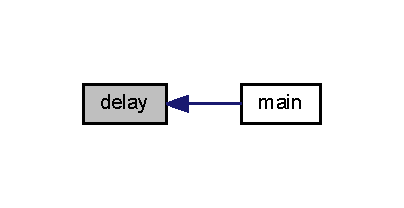
\includegraphics[width=194pt]{neslib_8h_a602d2b5e32479e0a80ad0d4dba8baf11_icgraph}
\end{center}
\end{figure}
\hypertarget{neslib_8h_a45b36ec1ac2e151ae56f3b1bc5dae73a}{}\label{neslib_8h_a45b36ec1ac2e151ae56f3b1bc5dae73a} 
\index{neslib.\+h@{neslib.\+h}!flush\+\_\+vram\+\_\+update@{flush\+\_\+vram\+\_\+update}}
\index{flush\+\_\+vram\+\_\+update@{flush\+\_\+vram\+\_\+update}!neslib.\+h@{neslib.\+h}}
\subsubsection{\texorpdfstring{flush\+\_\+vram\+\_\+update()}{flush\_vram\_update()}}
{\footnotesize\ttfamily void \+\_\+\+\_\+fastcall\+\_\+\+\_\+ flush\+\_\+vram\+\_\+update (\begin{DoxyParamCaption}\item[{unsigned char $\ast$}]{buf }\end{DoxyParamCaption})}

\hypertarget{neslib_8h_af821a6df3371ace281787bc921b3e1f9}{}\label{neslib_8h_af821a6df3371ace281787bc921b3e1f9} 
\index{neslib.\+h@{neslib.\+h}!memcpy@{memcpy}}
\index{memcpy@{memcpy}!neslib.\+h@{neslib.\+h}}
\subsubsection{\texorpdfstring{memcpy()}{memcpy()}}
{\footnotesize\ttfamily void \+\_\+\+\_\+fastcall\+\_\+\+\_\+ memcpy (\begin{DoxyParamCaption}\item[{void $\ast$}]{dst,  }\item[{void $\ast$}]{src,  }\item[{unsigned int}]{len }\end{DoxyParamCaption})}

\hypertarget{neslib_8h_a2e0070c87bd0f9fed3713a170f6387f3}{}\label{neslib_8h_a2e0070c87bd0f9fed3713a170f6387f3} 
\index{neslib.\+h@{neslib.\+h}!memfill@{memfill}}
\index{memfill@{memfill}!neslib.\+h@{neslib.\+h}}
\subsubsection{\texorpdfstring{memfill()}{memfill()}}
{\footnotesize\ttfamily void \+\_\+\+\_\+fastcall\+\_\+\+\_\+ memfill (\begin{DoxyParamCaption}\item[{void $\ast$}]{dst,  }\item[{unsigned char}]{value,  }\item[{unsigned int}]{len }\end{DoxyParamCaption})}

\hypertarget{neslib_8h_a7dc4007b9fa4154314ef56261351fa1b}{}\label{neslib_8h_a7dc4007b9fa4154314ef56261351fa1b} 
\index{neslib.\+h@{neslib.\+h}!music\+\_\+pause@{music\+\_\+pause}}
\index{music\+\_\+pause@{music\+\_\+pause}!neslib.\+h@{neslib.\+h}}
\subsubsection{\texorpdfstring{music\+\_\+pause()}{music\_pause()}}
{\footnotesize\ttfamily void \+\_\+\+\_\+fastcall\+\_\+\+\_\+ music\+\_\+pause (\begin{DoxyParamCaption}\item[{unsigned char}]{pause }\end{DoxyParamCaption})}

\hypertarget{neslib_8h_a4f8b0a8894cd7d8e7e2d4e9d190798b8}{}\label{neslib_8h_a4f8b0a8894cd7d8e7e2d4e9d190798b8} 
\index{neslib.\+h@{neslib.\+h}!music\+\_\+play@{music\+\_\+play}}
\index{music\+\_\+play@{music\+\_\+play}!neslib.\+h@{neslib.\+h}}
\subsubsection{\texorpdfstring{music\+\_\+play()}{music\_play()}}
{\footnotesize\ttfamily void \+\_\+\+\_\+fastcall\+\_\+\+\_\+ music\+\_\+play (\begin{DoxyParamCaption}\item[{unsigned char}]{song }\end{DoxyParamCaption})}

\hypertarget{neslib_8h_a1b9728244575ca5850ce93a6a581bef9}{}\label{neslib_8h_a1b9728244575ca5850ce93a6a581bef9} 
\index{neslib.\+h@{neslib.\+h}!music\+\_\+stop@{music\+\_\+stop}}
\index{music\+\_\+stop@{music\+\_\+stop}!neslib.\+h@{neslib.\+h}}
\subsubsection{\texorpdfstring{music\+\_\+stop()}{music\_stop()}}
{\footnotesize\ttfamily void \+\_\+\+\_\+fastcall\+\_\+\+\_\+ music\+\_\+stop (\begin{DoxyParamCaption}\item[{void}]{ }\end{DoxyParamCaption})}

\hypertarget{neslib_8h_af0e0aec75a3a9210d71775340297a652}{}\label{neslib_8h_af0e0aec75a3a9210d71775340297a652} 
\index{neslib.\+h@{neslib.\+h}!oam\+\_\+clear@{oam\+\_\+clear}}
\index{oam\+\_\+clear@{oam\+\_\+clear}!neslib.\+h@{neslib.\+h}}
\subsubsection{\texorpdfstring{oam\+\_\+clear()}{oam\_clear()}}
{\footnotesize\ttfamily void \+\_\+\+\_\+fastcall\+\_\+\+\_\+ oam\+\_\+clear (\begin{DoxyParamCaption}\item[{void}]{ }\end{DoxyParamCaption})}

Here is the caller graph for this function\+:\nopagebreak
\begin{figure}[H]
\begin{center}
\leavevmode
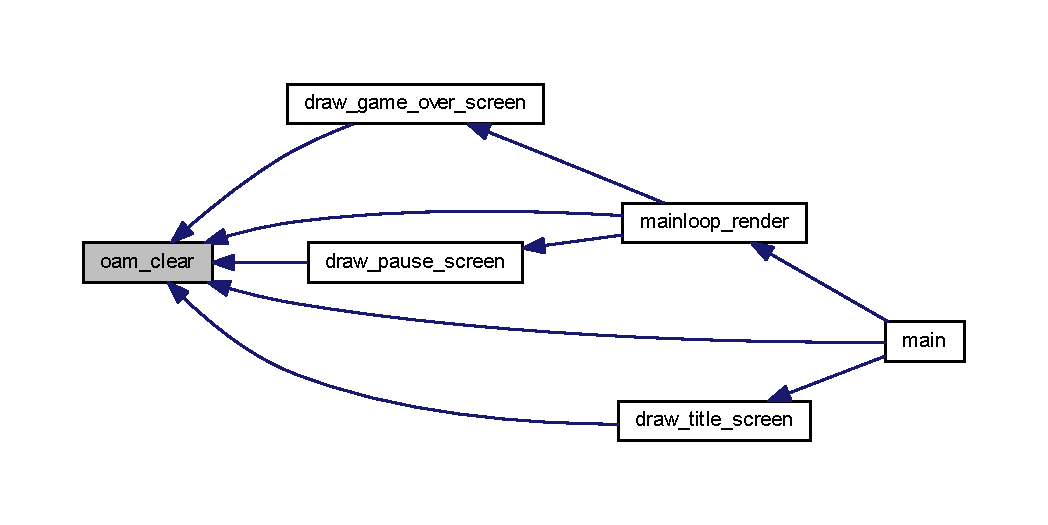
\includegraphics[width=350pt]{neslib_8h_af0e0aec75a3a9210d71775340297a652_icgraph}
\end{center}
\end{figure}
\hypertarget{neslib_8h_a5c88de00f4254f8afbf16a988cac23d5}{}\label{neslib_8h_a5c88de00f4254f8afbf16a988cac23d5} 
\index{neslib.\+h@{neslib.\+h}!oam\+\_\+hide\+\_\+rest@{oam\+\_\+hide\+\_\+rest}}
\index{oam\+\_\+hide\+\_\+rest@{oam\+\_\+hide\+\_\+rest}!neslib.\+h@{neslib.\+h}}
\subsubsection{\texorpdfstring{oam\+\_\+hide\+\_\+rest()}{oam\_hide\_rest()}}
{\footnotesize\ttfamily void \+\_\+\+\_\+fastcall\+\_\+\+\_\+ oam\+\_\+hide\+\_\+rest (\begin{DoxyParamCaption}\item[{unsigned char}]{sprid }\end{DoxyParamCaption})}

\hypertarget{neslib_8h_a7e209d6621f62aa5e9bab1ba0d326eeb}{}\label{neslib_8h_a7e209d6621f62aa5e9bab1ba0d326eeb} 
\index{neslib.\+h@{neslib.\+h}!oam\+\_\+meta\+\_\+spr@{oam\+\_\+meta\+\_\+spr}}
\index{oam\+\_\+meta\+\_\+spr@{oam\+\_\+meta\+\_\+spr}!neslib.\+h@{neslib.\+h}}
\subsubsection{\texorpdfstring{oam\+\_\+meta\+\_\+spr()}{oam\_meta\_spr()}}
{\footnotesize\ttfamily unsigned char \+\_\+\+\_\+fastcall\+\_\+\+\_\+ oam\+\_\+meta\+\_\+spr (\begin{DoxyParamCaption}\item[{unsigned char}]{x,  }\item[{unsigned char}]{y,  }\item[{unsigned char}]{sprid,  }\item[{const unsigned char $\ast$}]{data }\end{DoxyParamCaption})}

\hypertarget{neslib_8h_ae3b393a128f547af14c5fc3f90b02998}{}\label{neslib_8h_ae3b393a128f547af14c5fc3f90b02998} 
\index{neslib.\+h@{neslib.\+h}!oam\+\_\+size@{oam\+\_\+size}}
\index{oam\+\_\+size@{oam\+\_\+size}!neslib.\+h@{neslib.\+h}}
\subsubsection{\texorpdfstring{oam\+\_\+size()}{oam\_size()}}
{\footnotesize\ttfamily void \+\_\+\+\_\+fastcall\+\_\+\+\_\+ oam\+\_\+size (\begin{DoxyParamCaption}\item[{unsigned char}]{size }\end{DoxyParamCaption})}

\hypertarget{neslib_8h_a6c0a83ae05e30af1643fbaf224ab8d74}{}\label{neslib_8h_a6c0a83ae05e30af1643fbaf224ab8d74} 
\index{neslib.\+h@{neslib.\+h}!oam\+\_\+spr@{oam\+\_\+spr}}
\index{oam\+\_\+spr@{oam\+\_\+spr}!neslib.\+h@{neslib.\+h}}
\subsubsection{\texorpdfstring{oam\+\_\+spr()}{oam\_spr()}}
{\footnotesize\ttfamily unsigned char \+\_\+\+\_\+fastcall\+\_\+\+\_\+ oam\+\_\+spr (\begin{DoxyParamCaption}\item[{unsigned char}]{x,  }\item[{unsigned char}]{y,  }\item[{unsigned char}]{chrnum,  }\item[{unsigned char}]{attr,  }\item[{unsigned char}]{sprid }\end{DoxyParamCaption})}

Here is the caller graph for this function\+:\nopagebreak
\begin{figure}[H]
\begin{center}
\leavevmode
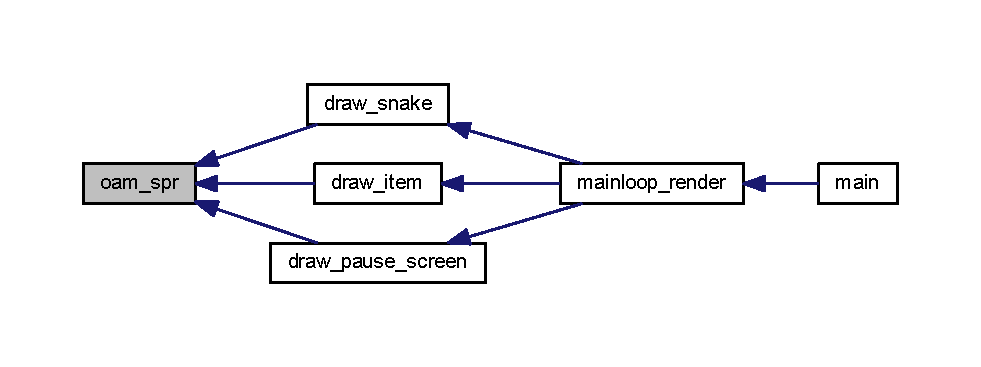
\includegraphics[width=350pt]{neslib_8h_a6c0a83ae05e30af1643fbaf224ab8d74_icgraph}
\end{center}
\end{figure}
\hypertarget{neslib_8h_ab3f58e98c2fdca9410fa342e1528a53c}{}\label{neslib_8h_ab3f58e98c2fdca9410fa342e1528a53c} 
\index{neslib.\+h@{neslib.\+h}!pad\+\_\+poll@{pad\+\_\+poll}}
\index{pad\+\_\+poll@{pad\+\_\+poll}!neslib.\+h@{neslib.\+h}}
\subsubsection{\texorpdfstring{pad\+\_\+poll()}{pad\_poll()}}
{\footnotesize\ttfamily unsigned char \+\_\+\+\_\+fastcall\+\_\+\+\_\+ pad\+\_\+poll (\begin{DoxyParamCaption}\item[{unsigned char}]{pad }\end{DoxyParamCaption})}

\hypertarget{neslib_8h_afdf5e93a522d447d124a0d73d9c91fd4}{}\label{neslib_8h_afdf5e93a522d447d124a0d73d9c91fd4} 
\index{neslib.\+h@{neslib.\+h}!pad\+\_\+state@{pad\+\_\+state}}
\index{pad\+\_\+state@{pad\+\_\+state}!neslib.\+h@{neslib.\+h}}
\subsubsection{\texorpdfstring{pad\+\_\+state()}{pad\_state()}}
{\footnotesize\ttfamily unsigned char \+\_\+\+\_\+fastcall\+\_\+\+\_\+ pad\+\_\+state (\begin{DoxyParamCaption}\item[{unsigned char}]{pad }\end{DoxyParamCaption})}

\hypertarget{neslib_8h_a73584a5b3af1517cb04f14c6118b5b0d}{}\label{neslib_8h_a73584a5b3af1517cb04f14c6118b5b0d} 
\index{neslib.\+h@{neslib.\+h}!pad\+\_\+trigger@{pad\+\_\+trigger}}
\index{pad\+\_\+trigger@{pad\+\_\+trigger}!neslib.\+h@{neslib.\+h}}
\subsubsection{\texorpdfstring{pad\+\_\+trigger()}{pad\_trigger()}}
{\footnotesize\ttfamily unsigned char \+\_\+\+\_\+fastcall\+\_\+\+\_\+ pad\+\_\+trigger (\begin{DoxyParamCaption}\item[{unsigned char}]{pad }\end{DoxyParamCaption})}

Here is the caller graph for this function\+:\nopagebreak
\begin{figure}[H]
\begin{center}
\leavevmode
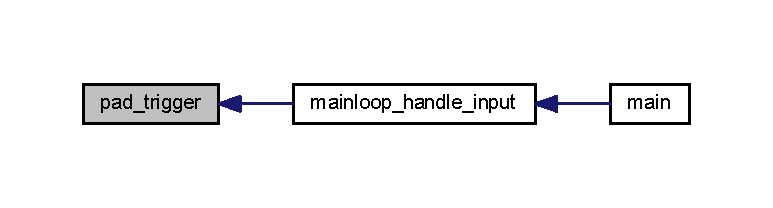
\includegraphics[width=350pt]{neslib_8h_a73584a5b3af1517cb04f14c6118b5b0d_icgraph}
\end{center}
\end{figure}
\hypertarget{neslib_8h_a8e6764b139f7b8482ca6f05cbe1cc55d}{}\label{neslib_8h_a8e6764b139f7b8482ca6f05cbe1cc55d} 
\index{neslib.\+h@{neslib.\+h}!pal\+\_\+all@{pal\+\_\+all}}
\index{pal\+\_\+all@{pal\+\_\+all}!neslib.\+h@{neslib.\+h}}
\subsubsection{\texorpdfstring{pal\+\_\+all()}{pal\_all()}}
{\footnotesize\ttfamily void \+\_\+\+\_\+fastcall\+\_\+\+\_\+ pal\+\_\+all (\begin{DoxyParamCaption}\item[{const char $\ast$}]{data }\end{DoxyParamCaption})}

\hypertarget{neslib_8h_a1f3f11758d2d0135f9451147e02f9f8f}{}\label{neslib_8h_a1f3f11758d2d0135f9451147e02f9f8f} 
\index{neslib.\+h@{neslib.\+h}!pal\+\_\+bg@{pal\+\_\+bg}}
\index{pal\+\_\+bg@{pal\+\_\+bg}!neslib.\+h@{neslib.\+h}}
\subsubsection{\texorpdfstring{pal\+\_\+bg()}{pal\_bg()}}
{\footnotesize\ttfamily void \+\_\+\+\_\+fastcall\+\_\+\+\_\+ pal\+\_\+bg (\begin{DoxyParamCaption}\item[{const char $\ast$}]{data }\end{DoxyParamCaption})}

Here is the caller graph for this function\+:\nopagebreak
\begin{figure}[H]
\begin{center}
\leavevmode
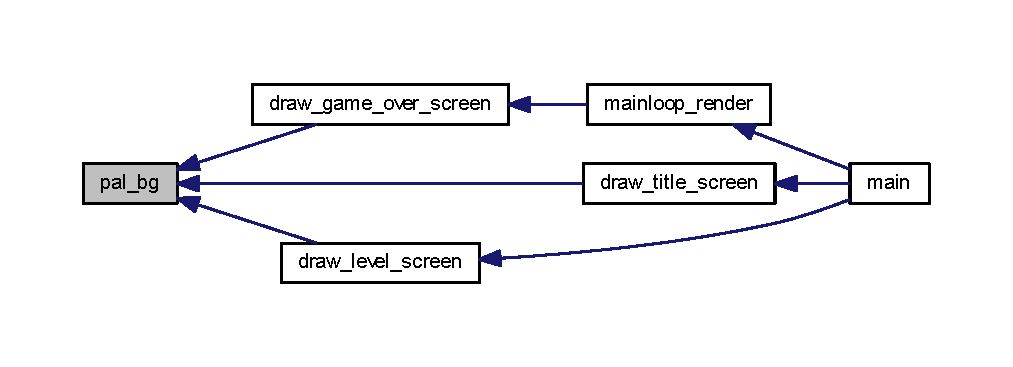
\includegraphics[width=350pt]{neslib_8h_a1f3f11758d2d0135f9451147e02f9f8f_icgraph}
\end{center}
\end{figure}
\hypertarget{neslib_8h_a9afa9017620492c47098497a628acd6a}{}\label{neslib_8h_a9afa9017620492c47098497a628acd6a} 
\index{neslib.\+h@{neslib.\+h}!pal\+\_\+bg\+\_\+bright@{pal\+\_\+bg\+\_\+bright}}
\index{pal\+\_\+bg\+\_\+bright@{pal\+\_\+bg\+\_\+bright}!neslib.\+h@{neslib.\+h}}
\subsubsection{\texorpdfstring{pal\+\_\+bg\+\_\+bright()}{pal\_bg\_bright()}}
{\footnotesize\ttfamily void \+\_\+\+\_\+fastcall\+\_\+\+\_\+ pal\+\_\+bg\+\_\+bright (\begin{DoxyParamCaption}\item[{unsigned char}]{bright }\end{DoxyParamCaption})}

\hypertarget{neslib_8h_a70af15380632618eeb4a79dd69d00f9b}{}\label{neslib_8h_a70af15380632618eeb4a79dd69d00f9b} 
\index{neslib.\+h@{neslib.\+h}!pal\+\_\+bright@{pal\+\_\+bright}}
\index{pal\+\_\+bright@{pal\+\_\+bright}!neslib.\+h@{neslib.\+h}}
\subsubsection{\texorpdfstring{pal\+\_\+bright()}{pal\_bright()}}
{\footnotesize\ttfamily void \+\_\+\+\_\+fastcall\+\_\+\+\_\+ pal\+\_\+bright (\begin{DoxyParamCaption}\item[{unsigned char}]{bright }\end{DoxyParamCaption})}

\hypertarget{neslib_8h_a94e96158db770e71b4d0df7243db92ce}{}\label{neslib_8h_a94e96158db770e71b4d0df7243db92ce} 
\index{neslib.\+h@{neslib.\+h}!pal\+\_\+clear@{pal\+\_\+clear}}
\index{pal\+\_\+clear@{pal\+\_\+clear}!neslib.\+h@{neslib.\+h}}
\subsubsection{\texorpdfstring{pal\+\_\+clear()}{pal\_clear()}}
{\footnotesize\ttfamily void \+\_\+\+\_\+fastcall\+\_\+\+\_\+ pal\+\_\+clear (\begin{DoxyParamCaption}\item[{void}]{ }\end{DoxyParamCaption})}

\hypertarget{neslib_8h_a2078d955183f42fc22631b945dd97076}{}\label{neslib_8h_a2078d955183f42fc22631b945dd97076} 
\index{neslib.\+h@{neslib.\+h}!pal\+\_\+col@{pal\+\_\+col}}
\index{pal\+\_\+col@{pal\+\_\+col}!neslib.\+h@{neslib.\+h}}
\subsubsection{\texorpdfstring{pal\+\_\+col()}{pal\_col()}}
{\footnotesize\ttfamily void \+\_\+\+\_\+fastcall\+\_\+\+\_\+ pal\+\_\+col (\begin{DoxyParamCaption}\item[{unsigned char}]{index,  }\item[{unsigned char}]{color }\end{DoxyParamCaption})}

\hypertarget{neslib_8h_a37b1ea3a9f615bf873ff1a9a7cb908e1}{}\label{neslib_8h_a37b1ea3a9f615bf873ff1a9a7cb908e1} 
\index{neslib.\+h@{neslib.\+h}!pal\+\_\+spr@{pal\+\_\+spr}}
\index{pal\+\_\+spr@{pal\+\_\+spr}!neslib.\+h@{neslib.\+h}}
\subsubsection{\texorpdfstring{pal\+\_\+spr()}{pal\_spr()}}
{\footnotesize\ttfamily void \+\_\+\+\_\+fastcall\+\_\+\+\_\+ pal\+\_\+spr (\begin{DoxyParamCaption}\item[{const char $\ast$}]{data }\end{DoxyParamCaption})}

Here is the caller graph for this function\+:\nopagebreak
\begin{figure}[H]
\begin{center}
\leavevmode
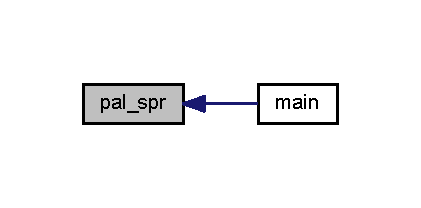
\includegraphics[width=202pt]{neslib_8h_a37b1ea3a9f615bf873ff1a9a7cb908e1_icgraph}
\end{center}
\end{figure}
\hypertarget{neslib_8h_a7d44d6e56989665ec6defb9a8506fe1b}{}\label{neslib_8h_a7d44d6e56989665ec6defb9a8506fe1b} 
\index{neslib.\+h@{neslib.\+h}!pal\+\_\+spr\+\_\+bright@{pal\+\_\+spr\+\_\+bright}}
\index{pal\+\_\+spr\+\_\+bright@{pal\+\_\+spr\+\_\+bright}!neslib.\+h@{neslib.\+h}}
\subsubsection{\texorpdfstring{pal\+\_\+spr\+\_\+bright()}{pal\_spr\_bright()}}
{\footnotesize\ttfamily void \+\_\+\+\_\+fastcall\+\_\+\+\_\+ pal\+\_\+spr\+\_\+bright (\begin{DoxyParamCaption}\item[{unsigned char}]{bright }\end{DoxyParamCaption})}

\hypertarget{neslib_8h_a210fdcdbafbb3eeb6df78df473b82c72}{}\label{neslib_8h_a210fdcdbafbb3eeb6df78df473b82c72} 
\index{neslib.\+h@{neslib.\+h}!ppu\+\_\+mask@{ppu\+\_\+mask}}
\index{ppu\+\_\+mask@{ppu\+\_\+mask}!neslib.\+h@{neslib.\+h}}
\subsubsection{\texorpdfstring{ppu\+\_\+mask()}{ppu\_mask()}}
{\footnotesize\ttfamily void \+\_\+\+\_\+fastcall\+\_\+\+\_\+ ppu\+\_\+mask (\begin{DoxyParamCaption}\item[{unsigned char}]{mask }\end{DoxyParamCaption})}

\hypertarget{neslib_8h_ae647495b7a80abff740f5e6169935faf}{}\label{neslib_8h_ae647495b7a80abff740f5e6169935faf} 
\index{neslib.\+h@{neslib.\+h}!ppu\+\_\+off@{ppu\+\_\+off}}
\index{ppu\+\_\+off@{ppu\+\_\+off}!neslib.\+h@{neslib.\+h}}
\subsubsection{\texorpdfstring{ppu\+\_\+off()}{ppu\_off()}}
{\footnotesize\ttfamily void \+\_\+\+\_\+fastcall\+\_\+\+\_\+ ppu\+\_\+off (\begin{DoxyParamCaption}\item[{void}]{ }\end{DoxyParamCaption})}

Here is the caller graph for this function\+:\nopagebreak
\begin{figure}[H]
\begin{center}
\leavevmode
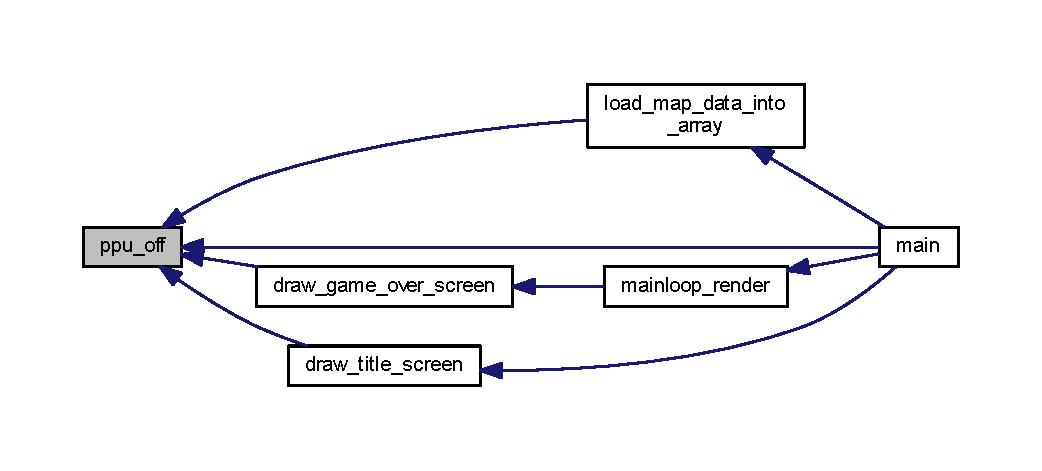
\includegraphics[width=350pt]{neslib_8h_ae647495b7a80abff740f5e6169935faf_icgraph}
\end{center}
\end{figure}
\hypertarget{neslib_8h_a67f5c6d5ee71fb0a59eb15526bc2cc84}{}\label{neslib_8h_a67f5c6d5ee71fb0a59eb15526bc2cc84} 
\index{neslib.\+h@{neslib.\+h}!ppu\+\_\+on\+\_\+all@{ppu\+\_\+on\+\_\+all}}
\index{ppu\+\_\+on\+\_\+all@{ppu\+\_\+on\+\_\+all}!neslib.\+h@{neslib.\+h}}
\subsubsection{\texorpdfstring{ppu\+\_\+on\+\_\+all()}{ppu\_on\_all()}}
{\footnotesize\ttfamily void \+\_\+\+\_\+fastcall\+\_\+\+\_\+ ppu\+\_\+on\+\_\+all (\begin{DoxyParamCaption}\item[{void}]{ }\end{DoxyParamCaption})}

Here is the caller graph for this function\+:\nopagebreak
\begin{figure}[H]
\begin{center}
\leavevmode
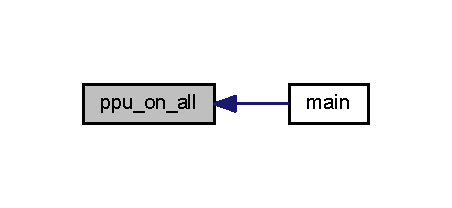
\includegraphics[width=217pt]{neslib_8h_a67f5c6d5ee71fb0a59eb15526bc2cc84_icgraph}
\end{center}
\end{figure}
\hypertarget{neslib_8h_ac75389467f7f5846f6bb433f658841f2}{}\label{neslib_8h_ac75389467f7f5846f6bb433f658841f2} 
\index{neslib.\+h@{neslib.\+h}!ppu\+\_\+on\+\_\+bg@{ppu\+\_\+on\+\_\+bg}}
\index{ppu\+\_\+on\+\_\+bg@{ppu\+\_\+on\+\_\+bg}!neslib.\+h@{neslib.\+h}}
\subsubsection{\texorpdfstring{ppu\+\_\+on\+\_\+bg()}{ppu\_on\_bg()}}
{\footnotesize\ttfamily void \+\_\+\+\_\+fastcall\+\_\+\+\_\+ ppu\+\_\+on\+\_\+bg (\begin{DoxyParamCaption}\item[{void}]{ }\end{DoxyParamCaption})}

Here is the caller graph for this function\+:\nopagebreak
\begin{figure}[H]
\begin{center}
\leavevmode
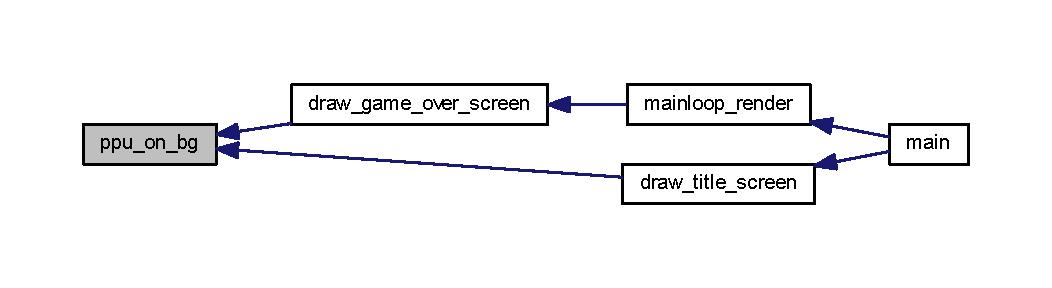
\includegraphics[width=350pt]{neslib_8h_ac75389467f7f5846f6bb433f658841f2_icgraph}
\end{center}
\end{figure}
\hypertarget{neslib_8h_aa3698cdae6c85c5e070cf969be67f18b}{}\label{neslib_8h_aa3698cdae6c85c5e070cf969be67f18b} 
\index{neslib.\+h@{neslib.\+h}!ppu\+\_\+on\+\_\+spr@{ppu\+\_\+on\+\_\+spr}}
\index{ppu\+\_\+on\+\_\+spr@{ppu\+\_\+on\+\_\+spr}!neslib.\+h@{neslib.\+h}}
\subsubsection{\texorpdfstring{ppu\+\_\+on\+\_\+spr()}{ppu\_on\_spr()}}
{\footnotesize\ttfamily void \+\_\+\+\_\+fastcall\+\_\+\+\_\+ ppu\+\_\+on\+\_\+spr (\begin{DoxyParamCaption}\item[{void}]{ }\end{DoxyParamCaption})}

\hypertarget{neslib_8h_ae02360a1a75a6888528a3d8b91fd2e05}{}\label{neslib_8h_ae02360a1a75a6888528a3d8b91fd2e05} 
\index{neslib.\+h@{neslib.\+h}!ppu\+\_\+system@{ppu\+\_\+system}}
\index{ppu\+\_\+system@{ppu\+\_\+system}!neslib.\+h@{neslib.\+h}}
\subsubsection{\texorpdfstring{ppu\+\_\+system()}{ppu\_system()}}
{\footnotesize\ttfamily unsigned char \+\_\+\+\_\+fastcall\+\_\+\+\_\+ ppu\+\_\+system (\begin{DoxyParamCaption}\item[{void}]{ }\end{DoxyParamCaption})}

\hypertarget{neslib_8h_af709dcf41df583b1cf97d17d2a999763}{}\label{neslib_8h_af709dcf41df583b1cf97d17d2a999763} 
\index{neslib.\+h@{neslib.\+h}!ppu\+\_\+wait\+\_\+frame@{ppu\+\_\+wait\+\_\+frame}}
\index{ppu\+\_\+wait\+\_\+frame@{ppu\+\_\+wait\+\_\+frame}!neslib.\+h@{neslib.\+h}}
\subsubsection{\texorpdfstring{ppu\+\_\+wait\+\_\+frame()}{ppu\_wait\_frame()}}
{\footnotesize\ttfamily void \+\_\+\+\_\+fastcall\+\_\+\+\_\+ ppu\+\_\+wait\+\_\+frame (\begin{DoxyParamCaption}\item[{void}]{ }\end{DoxyParamCaption})}

\hypertarget{neslib_8h_ac88eae7b7797eb87915966d9084eef03}{}\label{neslib_8h_ac88eae7b7797eb87915966d9084eef03} 
\index{neslib.\+h@{neslib.\+h}!ppu\+\_\+wait\+\_\+nmi@{ppu\+\_\+wait\+\_\+nmi}}
\index{ppu\+\_\+wait\+\_\+nmi@{ppu\+\_\+wait\+\_\+nmi}!neslib.\+h@{neslib.\+h}}
\subsubsection{\texorpdfstring{ppu\+\_\+wait\+\_\+nmi()}{ppu\_wait\_nmi()}}
{\footnotesize\ttfamily void \+\_\+\+\_\+fastcall\+\_\+\+\_\+ ppu\+\_\+wait\+\_\+nmi (\begin{DoxyParamCaption}\item[{void}]{ }\end{DoxyParamCaption})}

Here is the caller graph for this function\+:\nopagebreak
\begin{figure}[H]
\begin{center}
\leavevmode
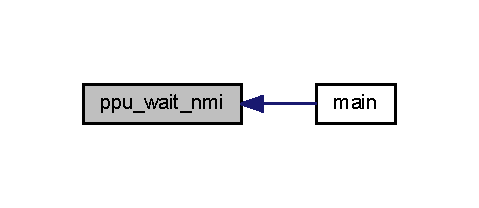
\includegraphics[width=230pt]{neslib_8h_ac88eae7b7797eb87915966d9084eef03_icgraph}
\end{center}
\end{figure}
\hypertarget{neslib_8h_a9882b1229885d6248b559b19897317ad}{}\label{neslib_8h_a9882b1229885d6248b559b19897317ad} 
\index{neslib.\+h@{neslib.\+h}!rand16@{rand16}}
\index{rand16@{rand16}!neslib.\+h@{neslib.\+h}}
\subsubsection{\texorpdfstring{rand16()}{rand16()}}
{\footnotesize\ttfamily unsigned int \+\_\+\+\_\+fastcall\+\_\+\+\_\+ rand16 (\begin{DoxyParamCaption}\item[{void}]{ }\end{DoxyParamCaption})}

\hypertarget{neslib_8h_a8fe1185fb429a4f9a0b82f9cd2c703e5}{}\label{neslib_8h_a8fe1185fb429a4f9a0b82f9cd2c703e5} 
\index{neslib.\+h@{neslib.\+h}!rand8@{rand8}}
\index{rand8@{rand8}!neslib.\+h@{neslib.\+h}}
\subsubsection{\texorpdfstring{rand8()}{rand8()}}
{\footnotesize\ttfamily unsigned char \+\_\+\+\_\+fastcall\+\_\+\+\_\+ rand8 (\begin{DoxyParamCaption}\item[{void}]{ }\end{DoxyParamCaption})}

Here is the caller graph for this function\+:\nopagebreak
\begin{figure}[H]
\begin{center}
\leavevmode
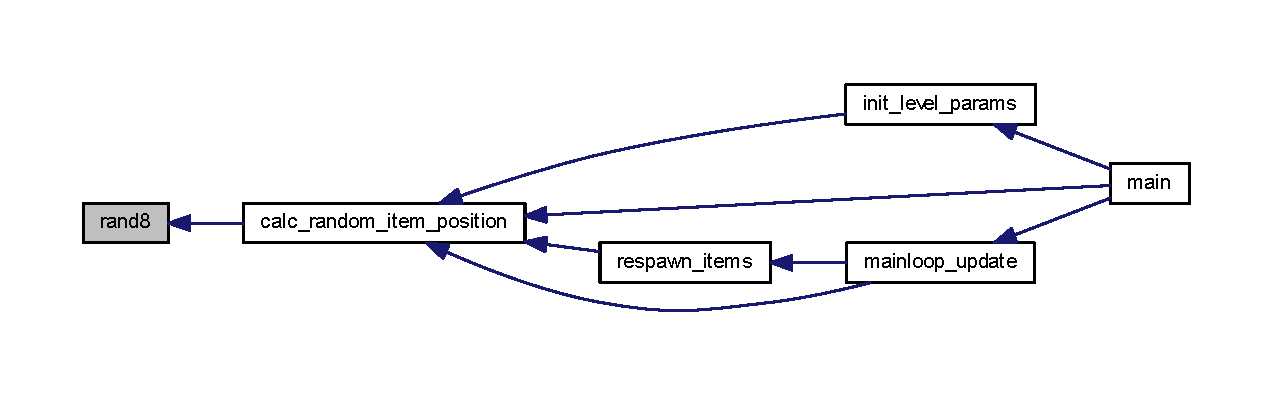
\includegraphics[width=350pt]{neslib_8h_a8fe1185fb429a4f9a0b82f9cd2c703e5_icgraph}
\end{center}
\end{figure}
\hypertarget{neslib_8h_aa446441cfacd18a332670718337e5115}{}\label{neslib_8h_aa446441cfacd18a332670718337e5115} 
\index{neslib.\+h@{neslib.\+h}!sample\+\_\+play@{sample\+\_\+play}}
\index{sample\+\_\+play@{sample\+\_\+play}!neslib.\+h@{neslib.\+h}}
\subsubsection{\texorpdfstring{sample\+\_\+play()}{sample\_play()}}
{\footnotesize\ttfamily void \+\_\+\+\_\+fastcall\+\_\+\+\_\+ sample\+\_\+play (\begin{DoxyParamCaption}\item[{unsigned char}]{sample }\end{DoxyParamCaption})}

\hypertarget{neslib_8h_a6dd1d8cbcb8005da1006cd8cb870c03e}{}\label{neslib_8h_a6dd1d8cbcb8005da1006cd8cb870c03e} 
\index{neslib.\+h@{neslib.\+h}!scroll@{scroll}}
\index{scroll@{scroll}!neslib.\+h@{neslib.\+h}}
\subsubsection{\texorpdfstring{scroll()}{scroll()}}
{\footnotesize\ttfamily void \+\_\+\+\_\+fastcall\+\_\+\+\_\+ scroll (\begin{DoxyParamCaption}\item[{unsigned int}]{x,  }\item[{unsigned int}]{y }\end{DoxyParamCaption})}

\hypertarget{neslib_8h_a4552535575cb708a9cd65053d31f1520}{}\label{neslib_8h_a4552535575cb708a9cd65053d31f1520} 
\index{neslib.\+h@{neslib.\+h}!set\+\_\+rand@{set\+\_\+rand}}
\index{set\+\_\+rand@{set\+\_\+rand}!neslib.\+h@{neslib.\+h}}
\subsubsection{\texorpdfstring{set\+\_\+rand()}{set\_rand()}}
{\footnotesize\ttfamily void \+\_\+\+\_\+fastcall\+\_\+\+\_\+ set\+\_\+rand (\begin{DoxyParamCaption}\item[{unsigned int}]{seed }\end{DoxyParamCaption})}

\hypertarget{neslib_8h_a025e06c022d08b2fa828e8e4597004c7}{}\label{neslib_8h_a025e06c022d08b2fa828e8e4597004c7} 
\index{neslib.\+h@{neslib.\+h}!set\+\_\+vram\+\_\+update@{set\+\_\+vram\+\_\+update}}
\index{set\+\_\+vram\+\_\+update@{set\+\_\+vram\+\_\+update}!neslib.\+h@{neslib.\+h}}
\subsubsection{\texorpdfstring{set\+\_\+vram\+\_\+update()}{set\_vram\_update()}}
{\footnotesize\ttfamily void \+\_\+\+\_\+fastcall\+\_\+\+\_\+ set\+\_\+vram\+\_\+update (\begin{DoxyParamCaption}\item[{unsigned char $\ast$}]{buf }\end{DoxyParamCaption})}

Here is the caller graph for this function\+:\nopagebreak
\begin{figure}[H]
\begin{center}
\leavevmode
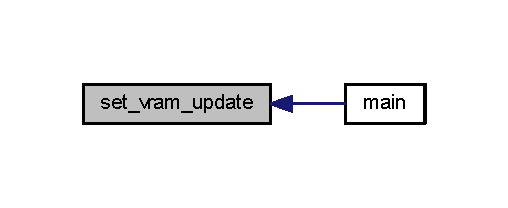
\includegraphics[width=244pt]{neslib_8h_a025e06c022d08b2fa828e8e4597004c7_icgraph}
\end{center}
\end{figure}
\hypertarget{neslib_8h_aeb2c4e716b2b6e9d31315ad4cec98623}{}\label{neslib_8h_aeb2c4e716b2b6e9d31315ad4cec98623} 
\index{neslib.\+h@{neslib.\+h}!sfx\+\_\+play@{sfx\+\_\+play}}
\index{sfx\+\_\+play@{sfx\+\_\+play}!neslib.\+h@{neslib.\+h}}
\subsubsection{\texorpdfstring{sfx\+\_\+play()}{sfx\_play()}}
{\footnotesize\ttfamily void \+\_\+\+\_\+fastcall\+\_\+\+\_\+ sfx\+\_\+play (\begin{DoxyParamCaption}\item[{unsigned char}]{sound,  }\item[{unsigned char}]{channel }\end{DoxyParamCaption})}

\hypertarget{neslib_8h_a684e5302447c159136256469bd224c69}{}\label{neslib_8h_a684e5302447c159136256469bd224c69} 
\index{neslib.\+h@{neslib.\+h}!split@{split}}
\index{split@{split}!neslib.\+h@{neslib.\+h}}
\subsubsection{\texorpdfstring{split()}{split()}}
{\footnotesize\ttfamily void \+\_\+\+\_\+fastcall\+\_\+\+\_\+ split (\begin{DoxyParamCaption}\item[{unsigned int}]{x,  }\item[{unsigned int}]{y }\end{DoxyParamCaption})}

\hypertarget{neslib_8h_a8460c4c927241500a3a09c245ceeea52}{}\label{neslib_8h_a8460c4c927241500a3a09c245ceeea52} 
\index{neslib.\+h@{neslib.\+h}!vram\+\_\+adr@{vram\+\_\+adr}}
\index{vram\+\_\+adr@{vram\+\_\+adr}!neslib.\+h@{neslib.\+h}}
\subsubsection{\texorpdfstring{vram\+\_\+adr()}{vram\_adr()}}
{\footnotesize\ttfamily void \+\_\+\+\_\+fastcall\+\_\+\+\_\+ vram\+\_\+adr (\begin{DoxyParamCaption}\item[{unsigned int}]{adr }\end{DoxyParamCaption})}

Here is the caller graph for this function\+:\nopagebreak
\begin{figure}[H]
\begin{center}
\leavevmode
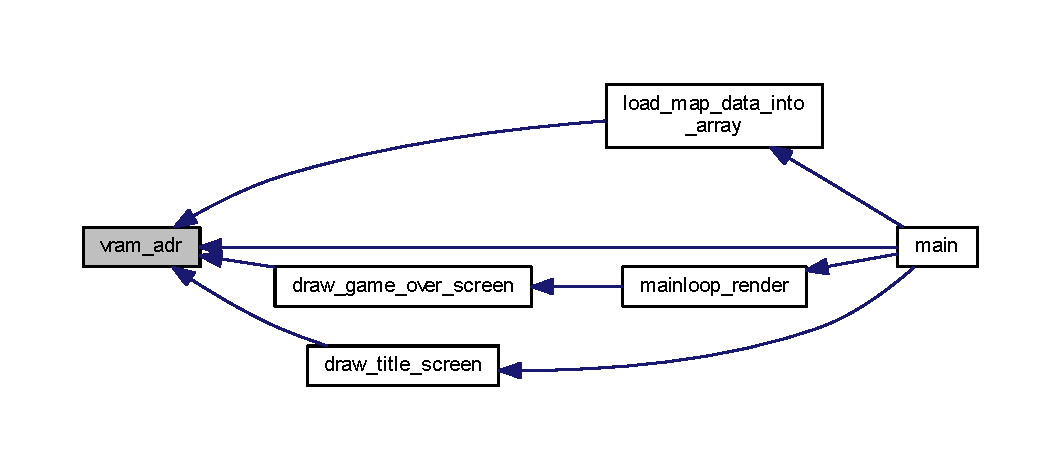
\includegraphics[width=350pt]{neslib_8h_a8460c4c927241500a3a09c245ceeea52_icgraph}
\end{center}
\end{figure}
\hypertarget{neslib_8h_a09eb5b41661ff3330648be48a85ff6d2}{}\label{neslib_8h_a09eb5b41661ff3330648be48a85ff6d2} 
\index{neslib.\+h@{neslib.\+h}!vram\+\_\+fill@{vram\+\_\+fill}}
\index{vram\+\_\+fill@{vram\+\_\+fill}!neslib.\+h@{neslib.\+h}}
\subsubsection{\texorpdfstring{vram\+\_\+fill()}{vram\_fill()}}
{\footnotesize\ttfamily void \+\_\+\+\_\+fastcall\+\_\+\+\_\+ vram\+\_\+fill (\begin{DoxyParamCaption}\item[{unsigned char}]{n,  }\item[{unsigned int}]{len }\end{DoxyParamCaption})}

\hypertarget{neslib_8h_ab567af57e7f8bf8bcfd403dd0e4a0e12}{}\label{neslib_8h_ab567af57e7f8bf8bcfd403dd0e4a0e12} 
\index{neslib.\+h@{neslib.\+h}!vram\+\_\+inc@{vram\+\_\+inc}}
\index{vram\+\_\+inc@{vram\+\_\+inc}!neslib.\+h@{neslib.\+h}}
\subsubsection{\texorpdfstring{vram\+\_\+inc()}{vram\_inc()}}
{\footnotesize\ttfamily void \+\_\+\+\_\+fastcall\+\_\+\+\_\+ vram\+\_\+inc (\begin{DoxyParamCaption}\item[{unsigned char}]{n }\end{DoxyParamCaption})}

\hypertarget{neslib_8h_a630a334d9ed2a4331a3b1168c7ffb466}{}\label{neslib_8h_a630a334d9ed2a4331a3b1168c7ffb466} 
\index{neslib.\+h@{neslib.\+h}!vram\+\_\+put@{vram\+\_\+put}}
\index{vram\+\_\+put@{vram\+\_\+put}!neslib.\+h@{neslib.\+h}}
\subsubsection{\texorpdfstring{vram\+\_\+put()}{vram\_put()}}
{\footnotesize\ttfamily void \+\_\+\+\_\+fastcall\+\_\+\+\_\+ vram\+\_\+put (\begin{DoxyParamCaption}\item[{unsigned char}]{n }\end{DoxyParamCaption})}

\hypertarget{neslib_8h_af14b2510268b3c13d9bd60837167bb09}{}\label{neslib_8h_af14b2510268b3c13d9bd60837167bb09} 
\index{neslib.\+h@{neslib.\+h}!vram\+\_\+read@{vram\+\_\+read}}
\index{vram\+\_\+read@{vram\+\_\+read}!neslib.\+h@{neslib.\+h}}
\subsubsection{\texorpdfstring{vram\+\_\+read()}{vram\_read()}}
{\footnotesize\ttfamily void \+\_\+\+\_\+fastcall\+\_\+\+\_\+ vram\+\_\+read (\begin{DoxyParamCaption}\item[{unsigned char $\ast$}]{dst,  }\item[{unsigned int}]{size }\end{DoxyParamCaption})}

Here is the caller graph for this function\+:\nopagebreak
\begin{figure}[H]
\begin{center}
\leavevmode
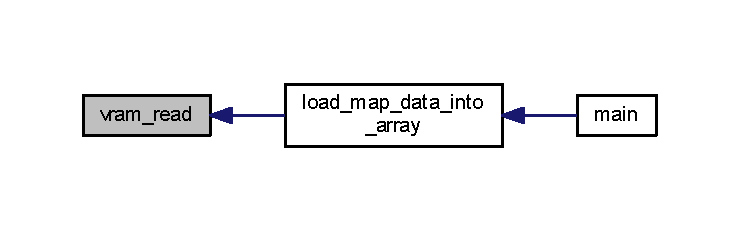
\includegraphics[width=350pt]{neslib_8h_af14b2510268b3c13d9bd60837167bb09_icgraph}
\end{center}
\end{figure}
\hypertarget{neslib_8h_a1adb35bc2bdf712c0b1b8223b72b1cb2}{}\label{neslib_8h_a1adb35bc2bdf712c0b1b8223b72b1cb2} 
\index{neslib.\+h@{neslib.\+h}!vram\+\_\+unrle@{vram\+\_\+unrle}}
\index{vram\+\_\+unrle@{vram\+\_\+unrle}!neslib.\+h@{neslib.\+h}}
\subsubsection{\texorpdfstring{vram\+\_\+unrle()}{vram\_unrle()}}
{\footnotesize\ttfamily void \+\_\+\+\_\+fastcall\+\_\+\+\_\+ vram\+\_\+unrle (\begin{DoxyParamCaption}\item[{const unsigned char $\ast$}]{data }\end{DoxyParamCaption})}

Here is the caller graph for this function\+:\nopagebreak
\begin{figure}[H]
\begin{center}
\leavevmode
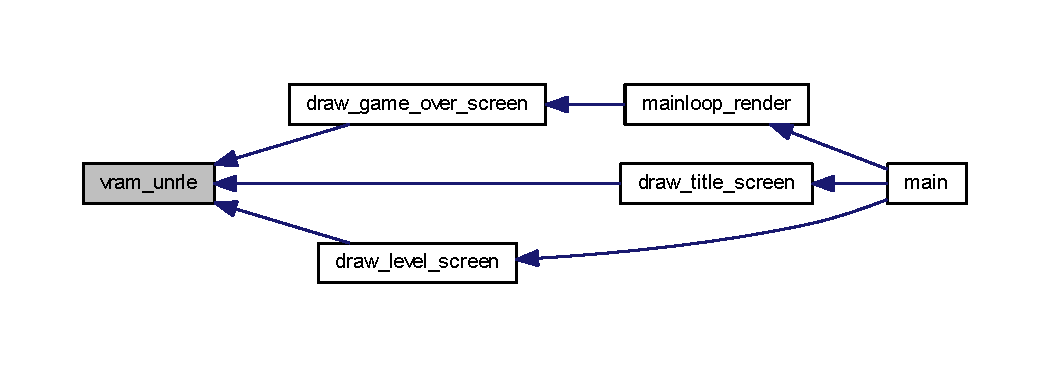
\includegraphics[width=350pt]{neslib_8h_a1adb35bc2bdf712c0b1b8223b72b1cb2_icgraph}
\end{center}
\end{figure}
\hypertarget{neslib_8h_af9982eb3cc548fcda10d53c8b29e4370}{}\label{neslib_8h_af9982eb3cc548fcda10d53c8b29e4370} 
\index{neslib.\+h@{neslib.\+h}!vram\+\_\+write@{vram\+\_\+write}}
\index{vram\+\_\+write@{vram\+\_\+write}!neslib.\+h@{neslib.\+h}}
\subsubsection{\texorpdfstring{vram\+\_\+write()}{vram\_write()}}
{\footnotesize\ttfamily void \+\_\+\+\_\+fastcall\+\_\+\+\_\+ vram\+\_\+write (\begin{DoxyParamCaption}\item[{unsigned char $\ast$}]{src,  }\item[{unsigned int}]{size }\end{DoxyParamCaption})}


\hypertarget{test__nam_8h}{}\section{C\+:/\+Users/\+Administrator/\+Documents/\+Git\+Hub/\+N\+E\+S-\/\+Snake/\+N\+E\+S\+Library/test\+\_\+nam.h File Reference}
\label{test__nam_8h}\index{C\+:/\+Users/\+Administrator/\+Documents/\+Git\+Hub/\+N\+E\+S-\/\+Snake/\+N\+E\+S\+Library/test\+\_\+nam.\+h@{C\+:/\+Users/\+Administrator/\+Documents/\+Git\+Hub/\+N\+E\+S-\/\+Snake/\+N\+E\+S\+Library/test\+\_\+nam.\+h}}
\subsection*{Variables}
\begin{DoxyCompactItemize}
\item 
const unsigned char \hyperlink{test__nam_8h_aa186951e3170721cab3dcc69129d4314}{test\+\_\+nam} \mbox{[}308\mbox{]}
\end{DoxyCompactItemize}


\subsection{Variable Documentation}
\hypertarget{test__nam_8h_aa186951e3170721cab3dcc69129d4314}{}\label{test__nam_8h_aa186951e3170721cab3dcc69129d4314} 
\index{test\+\_\+nam.\+h@{test\+\_\+nam.\+h}!test\+\_\+nam@{test\+\_\+nam}}
\index{test\+\_\+nam@{test\+\_\+nam}!test\+\_\+nam.\+h@{test\+\_\+nam.\+h}}
\subsubsection{\texorpdfstring{test\+\_\+nam}{test\_nam}}
{\footnotesize\ttfamily const unsigned char test\+\_\+nam\mbox{[}308\mbox{]}}

{\bfseries Initial value\+:}
\begin{DoxyCode}
=\{
0x01,0x00,0x01,0xa3,0x10,0x01,0x04,0x00,0x10,0x01,0x04,0x00,0x10,0x01,0x04,0x00,
0x10,0x01,0x04,0x00,0x01,0x0a,0x10,0x00,0x01,0x02,0x10,0x00,0x01,0x04,0x10,0x00,
0x01,0x06,0x10,0x00,0x01,0x0c,0x10,0x00,0x01,0x02,0x10,0x01,0x02,0x00,0x01,0x02,
0x10,0x01,0x04,0x00,0x01,0x02,0x10,0x00,0x01,0x0c,0x10,0x00,0x01,0x02,0x10,0x00,
0x01,0x08,0x10,0x00,0x01,0x02,0x10,0x00,0x01,0x0c,0x10,0x00,0x01,0x02,0x10,0x01,
0x04,0x00,0x10,0x01,0x04,0x00,0x01,0x02,0x10,0x00,0x01,0x42,0x10,0x00,0x01,0x06,
0x10,0x01,0x04,0x00,0x10,0x00,0x01,0x04,0x10,0x01,0x04,0x00,0x10,0x00,0x01,0x04,
0x10,0x00,0x01,0x06,0x10,0x00,0x01,0x02,0x10,0x00,0x10,0x00,0x01,0x04,0x10,0x00,
0x01,0x06,0x10,0x01,0x04,0x00,0x01,0x06,0x10,0x00,0x01,0x02,0x10,0x00,0x10,0x00,
0x01,0x04,0x10,0x01,0x02,0x00,0x01,0x04,0x10,0x00,0x01,0x02,0x10,0x00,0x01,0x06,
0x10,0x01,0x03,0x00,0x00,0x10,0x00,0x01,0x04,0x10,0x00,0x01,0x06,0x10,0x00,0x01,
0x02,0x10,0x00,0x01,0x06,0x10,0x00,0x01,0x02,0x10,0x00,0x10,0x01,0x04,0x00,0x10,
0x01,0x04,0x00,0x01,0x02,0x10,0x01,0x04,0x00,0x01,0x46,0x10,0x00,0x01,0x02,0x10,
0x00,0x10,0x01,0x04,0x00,0x10,0x01,0x04,0x00,0x01,0x0e,0x10,0x10,0x00,0x10,0x10,
0x00,0x10,0x00,0x01,0x02,0x10,0x00,0x10,0x00,0x01,0x02,0x10,0x00,0x01,0x0e,0x10,
0x00,0x10,0x00,0x10,0x00,0x10,0x00,0x01,0x02,0x10,0x00,0x10,0x00,0x01,0x02,0x10,
0x00,0x01,0x0e,0x10,0x00,0x01,0x02,0x10,0x00,0x10,0x01,0x04,0x00,0x10,0x01,0x04,
0x00,0x01,0x0e,0x10,0x00,0x01,0x02,0x10,0x00,0x10,0x00,0x01,0x02,0x10,0x00,0x10,
0x00,0x01,0xde,0x50,0x01,0x07,0x55,0x01,0x07,0xa5,0x01,0x07,0xaa,0x01,0x0f,0x0a,
0x01,0x07,0x01,0x00
\}
\end{DoxyCode}

\hypertarget{_r_e_a_d_m_e_8md}{}\section{C\+:/\+Users/\+Administrator/\+Documents/\+Git\+Hub/\+N\+E\+S-\/\+Snake/\+R\+E\+A\+D\+ME.md File Reference}
\label{_r_e_a_d_m_e_8md}\index{C\+:/\+Users/\+Administrator/\+Documents/\+Git\+Hub/\+N\+E\+S-\/\+Snake/\+R\+E\+A\+D\+M\+E.\+md@{C\+:/\+Users/\+Administrator/\+Documents/\+Git\+Hub/\+N\+E\+S-\/\+Snake/\+R\+E\+A\+D\+M\+E.\+md}}

\hypertarget{globals_8h}{}\section{C\+:/\+Users/\+Administrator/\+Documents/\+Git\+Hub/\+N\+E\+S-\/\+Snake/src/globals.h File Reference}
\label{globals_8h}\index{C\+:/\+Users/\+Administrator/\+Documents/\+Git\+Hub/\+N\+E\+S-\/\+Snake/src/globals.\+h@{C\+:/\+Users/\+Administrator/\+Documents/\+Git\+Hub/\+N\+E\+S-\/\+Snake/src/globals.\+h}}


This header file defines all global variables of the game.  


\subsection*{Variables}
\begin{DoxyCompactItemize}
\item 
static struct \hyperlink{structsnake__struct}{snake\+\_\+struct} \hyperlink{globals_8h_a9f760ea90d6dd23f945f328da2387297}{snake}
\end{DoxyCompactItemize}
\begin{Indent}{\bf Global variables, which are used to calculate pixel based coordinates (of body elements) to tile based coordinates.}\par
\begin{DoxyCompactItemize}
\item 
static unsigned char \hyperlink{globals_8h_a0f8633d0df266e6c86303410b4fd79b6}{tile\+\_\+x}
\item 
static unsigned char \hyperlink{globals_8h_a301ae8344e8d43b116d3aa6e19fd56ba}{tile\+\_\+y}
\end{DoxyCompactItemize}
\end{Indent}
\begin{Indent}{\bf Global variables, used to modify the background ingame}\par
\begin{DoxyCompactItemize}
\item 
static unsigned char \hyperlink{globals_8h_af1d853c79c2b46ff63daf4f811d7ce95}{update\+\_\+list} \mbox{[}5 $\ast$3+1\mbox{]}
\item 
static unsigned char $\ast$ \hyperlink{globals_8h_a493d790d010c98b6db7310b87faf8d05}{ul}
\end{DoxyCompactItemize}
\end{Indent}
\begin{Indent}{\bf Global variables, used for rendering sprites ingame}\par
\begin{DoxyCompactItemize}
\item 
static unsigned char \hyperlink{globals_8h_a4ffc86f06d1c7507f0a9079421ef75da}{sprite\+\_\+offset}
\end{DoxyCompactItemize}
\end{Indent}
\begin{Indent}{\bf Global variables, used for universal purpose e.\+g loops}\par
\begin{DoxyCompactItemize}
\item 
static unsigned char \hyperlink{globals_8h_a01494b8fd5801ba9e205324f4b1545ea}{i}
\item 
static unsigned char \hyperlink{globals_8h_aac1217779551b743f5645c17740178e3}{j}
\item 
static unsigned int \hyperlink{globals_8h_a90e096a39cfc6da042e02d27a346f2d3}{k}
\item 
static unsigned int \hyperlink{globals_8h_a3f724abfb9c2d5e84437c641786dcd70}{l}
\end{DoxyCompactItemize}
\end{Indent}
\begin{Indent}{\bf Global variables, used to interact with items}\par
\begin{DoxyCompactItemize}
\item 
static unsigned char \hyperlink{globals_8h_affca1b55c6470261c2b871273f1b604c}{item\+\_\+x}
\item 
static unsigned char \hyperlink{globals_8h_a126b314f52cc35faee4633c99042bf47}{item\+\_\+y}
\end{DoxyCompactItemize}
\end{Indent}
\begin{Indent}{\bf Global variables, used for game-\/states, menues, input}\par
\begin{DoxyCompactItemize}
\item 
static unsigned char \hyperlink{globals_8h_a4ca25633b87b17b67b540bc6eb28ecdd}{current\+\_\+level}
\item 
static unsigned char \hyperlink{globals_8h_a4c4b635fa72f98af449ca934c32c7b38}{max\+\_\+score}
\item 
static unsigned char \hyperlink{globals_8h_af005a22a9f7e1dbfe61f0c4380f5ce83}{pause}
\item 
static unsigned char \hyperlink{globals_8h_a474959fed45282f58d55114249dd04e1}{gameover}
\item 
static unsigned char \hyperlink{globals_8h_aec35dd4d246ba470806403dd75aba7b0}{input}
\item 
static unsigned char \hyperlink{globals_8h_a46d8dc26b0c7504baa3bd76429c0fe91}{pause\+\_\+loop}
\item 
static unsigned char \hyperlink{globals_8h_aa948973cb51e50909ae6ea85b7664767}{gameover\+\_\+loop}
\item 
static unsigned char \hyperlink{globals_8h_a050924f3d98ed7e3871436955ef669bd}{titlescreen}
\item 
static unsigned char \hyperlink{globals_8h_aaad902cba22507e143238f5671e8d234}{restart}
\end{DoxyCompactItemize}
\end{Indent}
\begin{Indent}{\bf Global variables, used to interact with the level map}\par
\begin{DoxyCompactItemize}
\item 
static unsigned char \hyperlink{globals_8h_a937f08b44e3e7c5d94de749012bc2a08}{map} \mbox{[}\hyperlink{macros_8h_aa037a6d6a4f04d51c7ec1c9ee9054e76}{M\+A\+P\+\_\+\+W\+I\+D\+TH} $\ast$\hyperlink{macros_8h_a529d5ebb449edf31d9835d13f4fb9f89}{M\+A\+P\+\_\+\+H\+E\+I\+G\+HT}\mbox{]}
\item 
static unsigned char \hyperlink{globals_8h_a2682880253356b9c35b2e6745c44f125}{name\+Row} \mbox{[}\hyperlink{macros_8h_aa037a6d6a4f04d51c7ec1c9ee9054e76}{M\+A\+P\+\_\+\+W\+I\+D\+TH}\mbox{]}
\item 
static unsigned int \hyperlink{globals_8h_a2656bd7f8fed8b98552f3a172c6f270e}{nametable\+\_\+fetch}
\end{DoxyCompactItemize}
\end{Indent}
\begin{Indent}{\bf List of the levels, include pointer to the packed nametable of the levels, menues, and pointer to the associated palette.}\par
\begin{DoxyCompactItemize}
\item 
const unsigned char $\ast$const \hyperlink{globals_8h_a3d77d32a3d5948ab26ad38f3c7d65d1d}{level\+List} \mbox{[}\hyperlink{macros_8h_a1a11e72c77f9f8e9fb4c27479f969626}{L\+E\+V\+E\+L\+S\+\_\+\+A\+LL}+2+2\mbox{]}
\end{DoxyCompactItemize}
\end{Indent}


\subsection{Detailed Description}
This header file defines all global variables of the game. 

\begin{DoxyAuthor}{Author}
Sebastian Dine 
\end{DoxyAuthor}


\subsection{Variable Documentation}
\hypertarget{globals_8h_a4ca25633b87b17b67b540bc6eb28ecdd}{}\label{globals_8h_a4ca25633b87b17b67b540bc6eb28ecdd} 
\index{globals.\+h@{globals.\+h}!current\+\_\+level@{current\+\_\+level}}
\index{current\+\_\+level@{current\+\_\+level}!globals.\+h@{globals.\+h}}
\subsubsection{\texorpdfstring{current\+\_\+level}{current\_level}}
{\footnotesize\ttfamily unsigned char current\+\_\+level\hspace{0.3cm}{\ttfamily [static]}}

Global variable, indicating the current level. \hypertarget{globals_8h_a474959fed45282f58d55114249dd04e1}{}\label{globals_8h_a474959fed45282f58d55114249dd04e1} 
\index{globals.\+h@{globals.\+h}!gameover@{gameover}}
\index{gameover@{gameover}!globals.\+h@{globals.\+h}}
\subsubsection{\texorpdfstring{gameover}{gameover}}
{\footnotesize\ttfamily unsigned char gameover\hspace{0.3cm}{\ttfamily [static]}}

Global variable, indicating the game over mode (1= game over 0= no game over). \hypertarget{globals_8h_aa948973cb51e50909ae6ea85b7664767}{}\label{globals_8h_aa948973cb51e50909ae6ea85b7664767} 
\index{globals.\+h@{globals.\+h}!gameover\+\_\+loop@{gameover\+\_\+loop}}
\index{gameover\+\_\+loop@{gameover\+\_\+loop}!globals.\+h@{globals.\+h}}
\subsubsection{\texorpdfstring{gameover\+\_\+loop}{gameover\_loop}}
{\footnotesize\ttfamily unsigned char gameover\+\_\+loop\hspace{0.3cm}{\ttfamily [static]}}

identifier to check, if first gameover loop is passed (1= true, 0= false). \hypertarget{globals_8h_a01494b8fd5801ba9e205324f4b1545ea}{}\label{globals_8h_a01494b8fd5801ba9e205324f4b1545ea} 
\index{globals.\+h@{globals.\+h}!i@{i}}
\index{i@{i}!globals.\+h@{globals.\+h}}
\subsubsection{\texorpdfstring{i}{i}}
{\footnotesize\ttfamily unsigned char i\hspace{0.3cm}{\ttfamily [static]}}

\hypertarget{globals_8h_aec35dd4d246ba470806403dd75aba7b0}{}\label{globals_8h_aec35dd4d246ba470806403dd75aba7b0} 
\index{globals.\+h@{globals.\+h}!input@{input}}
\index{input@{input}!globals.\+h@{globals.\+h}}
\subsubsection{\texorpdfstring{input}{input}}
{\footnotesize\ttfamily unsigned char input\hspace{0.3cm}{\ttfamily [static]}}

Global variable, holding the controller input of the current frame \hypertarget{globals_8h_affca1b55c6470261c2b871273f1b604c}{}\label{globals_8h_affca1b55c6470261c2b871273f1b604c} 
\index{globals.\+h@{globals.\+h}!item\+\_\+x@{item\+\_\+x}}
\index{item\+\_\+x@{item\+\_\+x}!globals.\+h@{globals.\+h}}
\subsubsection{\texorpdfstring{item\+\_\+x}{item\_x}}
{\footnotesize\ttfamily unsigned char item\+\_\+x\hspace{0.3cm}{\ttfamily [static]}}

\hypertarget{globals_8h_a126b314f52cc35faee4633c99042bf47}{}\label{globals_8h_a126b314f52cc35faee4633c99042bf47} 
\index{globals.\+h@{globals.\+h}!item\+\_\+y@{item\+\_\+y}}
\index{item\+\_\+y@{item\+\_\+y}!globals.\+h@{globals.\+h}}
\subsubsection{\texorpdfstring{item\+\_\+y}{item\_y}}
{\footnotesize\ttfamily unsigned char item\+\_\+y\hspace{0.3cm}{\ttfamily [static]}}

\hypertarget{globals_8h_aac1217779551b743f5645c17740178e3}{}\label{globals_8h_aac1217779551b743f5645c17740178e3} 
\index{globals.\+h@{globals.\+h}!j@{j}}
\index{j@{j}!globals.\+h@{globals.\+h}}
\subsubsection{\texorpdfstring{j}{j}}
{\footnotesize\ttfamily unsigned char j\hspace{0.3cm}{\ttfamily [static]}}

\hypertarget{globals_8h_a90e096a39cfc6da042e02d27a346f2d3}{}\label{globals_8h_a90e096a39cfc6da042e02d27a346f2d3} 
\index{globals.\+h@{globals.\+h}!k@{k}}
\index{k@{k}!globals.\+h@{globals.\+h}}
\subsubsection{\texorpdfstring{k}{k}}
{\footnotesize\ttfamily unsigned int k\hspace{0.3cm}{\ttfamily [static]}}

\hypertarget{globals_8h_a3f724abfb9c2d5e84437c641786dcd70}{}\label{globals_8h_a3f724abfb9c2d5e84437c641786dcd70} 
\index{globals.\+h@{globals.\+h}!l@{l}}
\index{l@{l}!globals.\+h@{globals.\+h}}
\subsubsection{\texorpdfstring{l}{l}}
{\footnotesize\ttfamily unsigned int l\hspace{0.3cm}{\ttfamily [static]}}

\hypertarget{globals_8h_a3d77d32a3d5948ab26ad38f3c7d65d1d}{}\label{globals_8h_a3d77d32a3d5948ab26ad38f3c7d65d1d} 
\index{globals.\+h@{globals.\+h}!level\+List@{level\+List}}
\index{level\+List@{level\+List}!globals.\+h@{globals.\+h}}
\subsubsection{\texorpdfstring{level\+List}{levelList}}
{\footnotesize\ttfamily const unsigned char$\ast$ const level\+List\mbox{[}\hyperlink{macros_8h_a1a11e72c77f9f8e9fb4c27479f969626}{L\+E\+V\+E\+L\+S\+\_\+\+A\+LL}+2+2\mbox{]}}

{\bfseries Initial value\+:}
\begin{DoxyCode}
=\{
    \hyperlink{level1__nam_8h_ae1585c8a4bd0ed3a7e1954654c7d25fb}{level1\_nam}, \hyperlink{level2__nam_8h_a1bd83e2d284faa101ea18d6e646b2a08}{level2\_nam},
    \hyperlink{game__over__nam_8h_adfee526430359e813aef4ebf5afe5b1c}{game\_over\_nam}, \hyperlink{titlescreen__nam_8h_a06862ae3bc1cd77a6d3a6b5372bcf89e}{titlescreen\_nam},
    \hyperlink{levels__pal_8h_a44ac48608bb3b86935fae3bdbdda8063}{levels\_pal}, \hyperlink{menue__pal_8h_a600954b5bbf9585ff21dfe398314f60d}{menue\_pal}
\}
\end{DoxyCode}
\hypertarget{globals_8h_a937f08b44e3e7c5d94de749012bc2a08}{}\label{globals_8h_a937f08b44e3e7c5d94de749012bc2a08} 
\index{globals.\+h@{globals.\+h}!map@{map}}
\index{map@{map}!globals.\+h@{globals.\+h}}
\subsubsection{\texorpdfstring{map}{map}}
{\footnotesize\ttfamily unsigned char map\mbox{[}\hyperlink{macros_8h_aa037a6d6a4f04d51c7ec1c9ee9054e76}{M\+A\+P\+\_\+\+W\+I\+D\+TH} $\ast$\hyperlink{macros_8h_a529d5ebb449edf31d9835d13f4fb9f89}{M\+A\+P\+\_\+\+H\+E\+I\+G\+HT}\mbox{]}\hspace{0.3cm}{\ttfamily [static]}}

Array of the complete game map (tile-\/based). \hypertarget{globals_8h_a4c4b635fa72f98af449ca934c32c7b38}{}\label{globals_8h_a4c4b635fa72f98af449ca934c32c7b38} 
\index{globals.\+h@{globals.\+h}!max\+\_\+score@{max\+\_\+score}}
\index{max\+\_\+score@{max\+\_\+score}!globals.\+h@{globals.\+h}}
\subsubsection{\texorpdfstring{max\+\_\+score}{max\_score}}
{\footnotesize\ttfamily unsigned char max\+\_\+score\hspace{0.3cm}{\ttfamily [static]}}

Global variable, indicating the maximum score of the current level. \hypertarget{globals_8h_a2682880253356b9c35b2e6745c44f125}{}\label{globals_8h_a2682880253356b9c35b2e6745c44f125} 
\index{globals.\+h@{globals.\+h}!name\+Row@{name\+Row}}
\index{name\+Row@{name\+Row}!globals.\+h@{globals.\+h}}
\subsubsection{\texorpdfstring{name\+Row}{nameRow}}
{\footnotesize\ttfamily unsigned char name\+Row\mbox{[}\hyperlink{macros_8h_aa037a6d6a4f04d51c7ec1c9ee9054e76}{M\+A\+P\+\_\+\+W\+I\+D\+TH}\mbox{]}\hspace{0.3cm}{\ttfamily [static]}}

Array for fetching nametable into array \textquotesingle{}map\textquotesingle{}, row by row. \hypertarget{globals_8h_a2656bd7f8fed8b98552f3a172c6f270e}{}\label{globals_8h_a2656bd7f8fed8b98552f3a172c6f270e} 
\index{globals.\+h@{globals.\+h}!nametable\+\_\+fetch@{nametable\+\_\+fetch}}
\index{nametable\+\_\+fetch@{nametable\+\_\+fetch}!globals.\+h@{globals.\+h}}
\subsubsection{\texorpdfstring{nametable\+\_\+fetch}{nametable\_fetch}}
{\footnotesize\ttfamily unsigned int nametable\+\_\+fetch\hspace{0.3cm}{\ttfamily [static]}}

Variable for fetching through nametable. \hypertarget{globals_8h_af005a22a9f7e1dbfe61f0c4380f5ce83}{}\label{globals_8h_af005a22a9f7e1dbfe61f0c4380f5ce83} 
\index{globals.\+h@{globals.\+h}!pause@{pause}}
\index{pause@{pause}!globals.\+h@{globals.\+h}}
\subsubsection{\texorpdfstring{pause}{pause}}
{\footnotesize\ttfamily unsigned char pause\hspace{0.3cm}{\ttfamily [static]}}

Global variable, indicating the pause mode (1= pause, 0= no pause). \hypertarget{globals_8h_a46d8dc26b0c7504baa3bd76429c0fe91}{}\label{globals_8h_a46d8dc26b0c7504baa3bd76429c0fe91} 
\index{globals.\+h@{globals.\+h}!pause\+\_\+loop@{pause\+\_\+loop}}
\index{pause\+\_\+loop@{pause\+\_\+loop}!globals.\+h@{globals.\+h}}
\subsubsection{\texorpdfstring{pause\+\_\+loop}{pause\_loop}}
{\footnotesize\ttfamily unsigned char pause\+\_\+loop\hspace{0.3cm}{\ttfamily [static]}}

Identifier to check, if first pause-\/loop is passed (1= true, 0= false). \hypertarget{globals_8h_aaad902cba22507e143238f5671e8d234}{}\label{globals_8h_aaad902cba22507e143238f5671e8d234} 
\index{globals.\+h@{globals.\+h}!restart@{restart}}
\index{restart@{restart}!globals.\+h@{globals.\+h}}
\subsubsection{\texorpdfstring{restart}{restart}}
{\footnotesize\ttfamily unsigned char restart\hspace{0.3cm}{\ttfamily [static]}}

Global variable, for handling the restart input \hypertarget{globals_8h_a9f760ea90d6dd23f945f328da2387297}{}\label{globals_8h_a9f760ea90d6dd23f945f328da2387297} 
\index{globals.\+h@{globals.\+h}!snake@{snake}}
\index{snake@{snake}!globals.\+h@{globals.\+h}}
\subsubsection{\texorpdfstring{snake}{snake}}
{\footnotesize\ttfamily struct \hyperlink{structsnake__struct}{snake\+\_\+struct} snake\hspace{0.3cm}{\ttfamily [static]}}

Global variable, containing all elements used to interact and display the snake \hypertarget{globals_8h_a4ffc86f06d1c7507f0a9079421ef75da}{}\label{globals_8h_a4ffc86f06d1c7507f0a9079421ef75da} 
\index{globals.\+h@{globals.\+h}!sprite\+\_\+offset@{sprite\+\_\+offset}}
\index{sprite\+\_\+offset@{sprite\+\_\+offset}!globals.\+h@{globals.\+h}}
\subsubsection{\texorpdfstring{sprite\+\_\+offset}{sprite\_offset}}
{\footnotesize\ttfamily unsigned char sprite\+\_\+offset\hspace{0.3cm}{\ttfamily [static]}}

\hypertarget{globals_8h_a0f8633d0df266e6c86303410b4fd79b6}{}\label{globals_8h_a0f8633d0df266e6c86303410b4fd79b6} 
\index{globals.\+h@{globals.\+h}!tile\+\_\+x@{tile\+\_\+x}}
\index{tile\+\_\+x@{tile\+\_\+x}!globals.\+h@{globals.\+h}}
\subsubsection{\texorpdfstring{tile\+\_\+x}{tile\_x}}
{\footnotesize\ttfamily unsigned char tile\+\_\+x\hspace{0.3cm}{\ttfamily [static]}}

\hypertarget{globals_8h_a301ae8344e8d43b116d3aa6e19fd56ba}{}\label{globals_8h_a301ae8344e8d43b116d3aa6e19fd56ba} 
\index{globals.\+h@{globals.\+h}!tile\+\_\+y@{tile\+\_\+y}}
\index{tile\+\_\+y@{tile\+\_\+y}!globals.\+h@{globals.\+h}}
\subsubsection{\texorpdfstring{tile\+\_\+y}{tile\_y}}
{\footnotesize\ttfamily unsigned char tile\+\_\+y\hspace{0.3cm}{\ttfamily [static]}}

\hypertarget{globals_8h_a050924f3d98ed7e3871436955ef669bd}{}\label{globals_8h_a050924f3d98ed7e3871436955ef669bd} 
\index{globals.\+h@{globals.\+h}!titlescreen@{titlescreen}}
\index{titlescreen@{titlescreen}!globals.\+h@{globals.\+h}}
\subsubsection{\texorpdfstring{titlescreen}{titlescreen}}
{\footnotesize\ttfamily unsigned char titlescreen\hspace{0.3cm}{\ttfamily [static]}}

Global variable, indicating the titlescreen mode (1=titlescreen 0= no titlescreen). \hypertarget{globals_8h_a493d790d010c98b6db7310b87faf8d05}{}\label{globals_8h_a493d790d010c98b6db7310b87faf8d05} 
\index{globals.\+h@{globals.\+h}!ul@{ul}}
\index{ul@{ul}!globals.\+h@{globals.\+h}}
\subsubsection{\texorpdfstring{ul}{ul}}
{\footnotesize\ttfamily unsigned char$\ast$ ul\hspace{0.3cm}{\ttfamily [static]}}

Pointer to array \textquotesingle{}update\+\_\+list\textquotesingle{} to enable better handling of the list \hypertarget{globals_8h_af1d853c79c2b46ff63daf4f811d7ce95}{}\label{globals_8h_af1d853c79c2b46ff63daf4f811d7ce95} 
\index{globals.\+h@{globals.\+h}!update\+\_\+list@{update\+\_\+list}}
\index{update\+\_\+list@{update\+\_\+list}!globals.\+h@{globals.\+h}}
\subsubsection{\texorpdfstring{update\+\_\+list}{update\_list}}
{\footnotesize\ttfamily unsigned char update\+\_\+list\mbox{[}5 $\ast$3+1\mbox{]}\hspace{0.3cm}{\ttfamily [static]}}

Array of bg-\/elements which will be used to update V\+R\+AM once per frame. Every 3 entries are describing one bg-\/element.
\begin{DoxyItemize}
\item the first 3 elements (9 array-\/elements) are assigned to the game score
\item the 4. and 5. element are assigned to the first and last body element of the snake
\item the last array-\/element needs to be the V\+R\+AM end-\/of-\/file-\/indicator N\+T\+\_\+\+U\+P\+D\+\_\+\+E\+OF.
\end{DoxyItemize}

Only two body elements need to be updated once per frame\+:
\begin{DoxyItemize}
\item The new first body element needs to be drawn
\item The old last body element need to be disabled 
\end{DoxyItemize}
\hypertarget{init_8c}{}\section{C\+:/\+Users/\+Administrator/\+Documents/\+Git\+Hub/\+N\+E\+S-\/\+Snake/src/init.c File Reference}
\label{init_8c}\index{C\+:/\+Users/\+Administrator/\+Documents/\+Git\+Hub/\+N\+E\+S-\/\+Snake/src/init.\+c@{C\+:/\+Users/\+Administrator/\+Documents/\+Git\+Hub/\+N\+E\+S-\/\+Snake/src/init.\+c}}


This file contains functions for initializing game elements.  


\subsection*{Functions}
\begin{DoxyCompactItemize}
\item 
void \hyperlink{init_8c_a0d12efc5b710644e3c76ceafe1b4f903}{load\+\_\+map\+\_\+data\+\_\+into\+\_\+array} (void)
\item 
void \hyperlink{init_8c_a2c5205e4618e0f665b8732c538418639}{init\+\_\+level\+\_\+params} (void)
\end{DoxyCompactItemize}


\subsection{Detailed Description}
This file contains functions for initializing game elements. 

\begin{DoxyAuthor}{Author}
Sebastian Dine 
\end{DoxyAuthor}


\subsection{Function Documentation}
\hypertarget{init_8c_a2c5205e4618e0f665b8732c538418639}{}\label{init_8c_a2c5205e4618e0f665b8732c538418639} 
\index{init.\+c@{init.\+c}!init\+\_\+level\+\_\+params@{init\+\_\+level\+\_\+params}}
\index{init\+\_\+level\+\_\+params@{init\+\_\+level\+\_\+params}!init.\+c@{init.\+c}}
\subsubsection{\texorpdfstring{init\+\_\+level\+\_\+params()}{init\_level\_params()}}
{\footnotesize\ttfamily void init\+\_\+level\+\_\+params (\begin{DoxyParamCaption}\item[{void}]{ }\end{DoxyParamCaption})}

This function initializes game elements, which differ between levels. (e.\+g. score to reach for next level or start position of the snake) Here is the caller graph for this function\+:\nopagebreak
\begin{figure}[H]
\begin{center}
\leavevmode
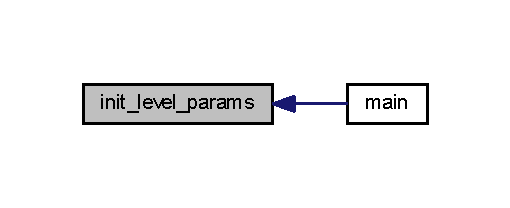
\includegraphics[width=245pt]{init_8c_a2c5205e4618e0f665b8732c538418639_icgraph}
\end{center}
\end{figure}
\hypertarget{init_8c_a0d12efc5b710644e3c76ceafe1b4f903}{}\label{init_8c_a0d12efc5b710644e3c76ceafe1b4f903} 
\index{init.\+c@{init.\+c}!load\+\_\+map\+\_\+data\+\_\+into\+\_\+array@{load\+\_\+map\+\_\+data\+\_\+into\+\_\+array}}
\index{load\+\_\+map\+\_\+data\+\_\+into\+\_\+array@{load\+\_\+map\+\_\+data\+\_\+into\+\_\+array}!init.\+c@{init.\+c}}
\subsubsection{\texorpdfstring{load\+\_\+map\+\_\+data\+\_\+into\+\_\+array()}{load\_map\_data\_into\_array()}}
{\footnotesize\ttfamily void load\+\_\+map\+\_\+data\+\_\+into\+\_\+array (\begin{DoxyParamCaption}\item[{void}]{ }\end{DoxyParamCaption})}

This function reads the namespace into global array \textquotesingle{}map\textquotesingle{}, which is used for further calculations, e.\+g. collision detection.

\begin{DoxyAuthor}{Author}
Sebastian Dine 
\end{DoxyAuthor}
Here is the call graph for this function\+:\nopagebreak
\begin{figure}[H]
\begin{center}
\leavevmode
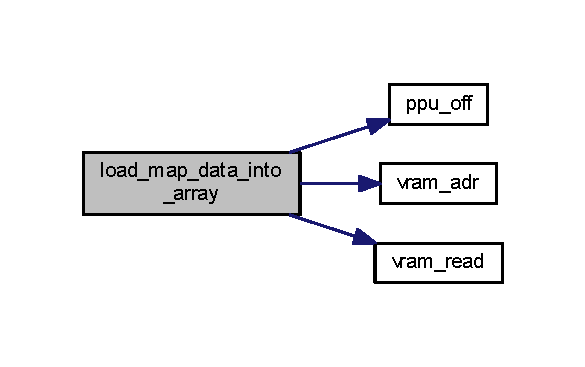
\includegraphics[width=281pt]{init_8c_a0d12efc5b710644e3c76ceafe1b4f903_cgraph}
\end{center}
\end{figure}
Here is the caller graph for this function\+:\nopagebreak
\begin{figure}[H]
\begin{center}
\leavevmode
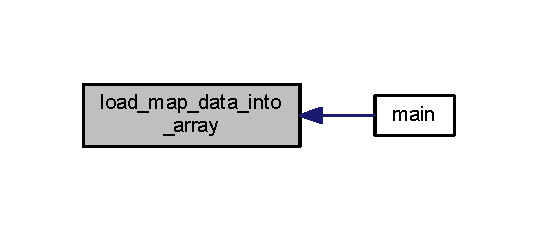
\includegraphics[width=258pt]{init_8c_a0d12efc5b710644e3c76ceafe1b4f903_icgraph}
\end{center}
\end{figure}

\hypertarget{input_8c}{}\section{C\+:/\+Users/\+Administrator/\+Documents/\+Git\+Hub/\+N\+E\+S-\/\+Snake/src/input.c File Reference}
\label{input_8c}\index{C\+:/\+Users/\+Administrator/\+Documents/\+Git\+Hub/\+N\+E\+S-\/\+Snake/src/input.\+c@{C\+:/\+Users/\+Administrator/\+Documents/\+Git\+Hub/\+N\+E\+S-\/\+Snake/src/input.\+c}}


This file contains functions for input handling from a controller.  


\subsection*{Functions}
\begin{DoxyCompactItemize}
\item 
void \hyperlink{input_8c_a8bf87fe078154e7e046e88a4d05e3e8c}{input\+\_\+btn\+\_\+start} (void)
\item 
void \hyperlink{input_8c_a42040f54ae307c565d4142f864d926c7}{mainloop\+\_\+handle\+\_\+input} (void)
\end{DoxyCompactItemize}


\subsection{Detailed Description}
This file contains functions for input handling from a controller. 

\begin{DoxyAuthor}{Author}
Sebastian Dine 
\end{DoxyAuthor}


\subsection{Function Documentation}
\hypertarget{input_8c_a8bf87fe078154e7e046e88a4d05e3e8c}{}\label{input_8c_a8bf87fe078154e7e046e88a4d05e3e8c} 
\index{input.\+c@{input.\+c}!input\+\_\+btn\+\_\+start@{input\+\_\+btn\+\_\+start}}
\index{input\+\_\+btn\+\_\+start@{input\+\_\+btn\+\_\+start}!input.\+c@{input.\+c}}
\subsubsection{\texorpdfstring{input\+\_\+btn\+\_\+start()}{input\_btn\_start()}}
{\footnotesize\ttfamily void input\+\_\+btn\+\_\+start (\begin{DoxyParamCaption}\item[{void}]{ }\end{DoxyParamCaption})}

This function contains the logic for the S\+T\+A\+RT button according to different scenarios e.\+g. title screen, ingame, gameover.

\begin{DoxyAuthor}{Author}
Sebastian Dine 
\end{DoxyAuthor}
Here is the caller graph for this function\+:\nopagebreak
\begin{figure}[H]
\begin{center}
\leavevmode
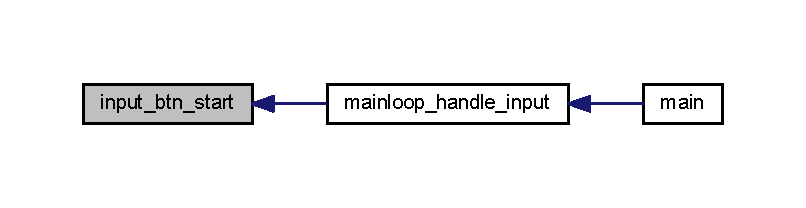
\includegraphics[width=350pt]{input_8c_a8bf87fe078154e7e046e88a4d05e3e8c_icgraph}
\end{center}
\end{figure}
\hypertarget{input_8c_a42040f54ae307c565d4142f864d926c7}{}\label{input_8c_a42040f54ae307c565d4142f864d926c7} 
\index{input.\+c@{input.\+c}!mainloop\+\_\+handle\+\_\+input@{mainloop\+\_\+handle\+\_\+input}}
\index{mainloop\+\_\+handle\+\_\+input@{mainloop\+\_\+handle\+\_\+input}!input.\+c@{input.\+c}}
\subsubsection{\texorpdfstring{mainloop\+\_\+handle\+\_\+input()}{mainloop\_handle\_input()}}
{\footnotesize\ttfamily void mainloop\+\_\+handle\+\_\+input (\begin{DoxyParamCaption}\item[{void}]{ }\end{DoxyParamCaption})}

This function provides the main input handling functionalities for an controller on port 1. It contains logic for input of the following buttons\+: UP, D\+O\+WN, L\+E\+FT, R\+I\+G\+HT, S\+T\+A\+RT.

\begin{DoxyAuthor}{Author}
Sebastian Dine 
\end{DoxyAuthor}
Here is the call graph for this function\+:\nopagebreak
\begin{figure}[H]
\begin{center}
\leavevmode
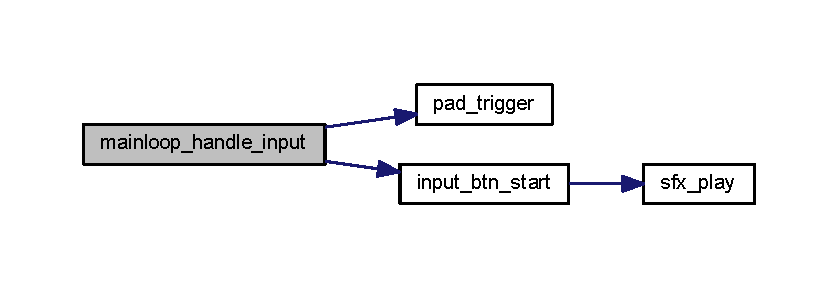
\includegraphics[width=313pt]{input_8c_a42040f54ae307c565d4142f864d926c7_cgraph}
\end{center}
\end{figure}
Here is the caller graph for this function\+:\nopagebreak
\begin{figure}[H]
\begin{center}
\leavevmode
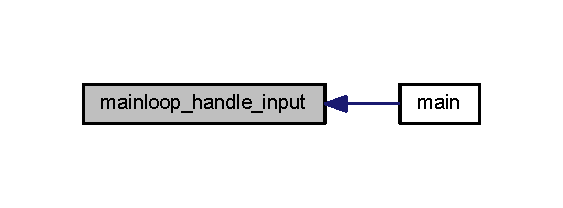
\includegraphics[width=270pt]{input_8c_a42040f54ae307c565d4142f864d926c7_icgraph}
\end{center}
\end{figure}

\hypertarget{macros_8h}{}\section{C\+:/\+Users/\+Administrator/\+Documents/\+Git\+Hub/\+N\+E\+S-\/\+Snake/src/macros.h File Reference}
\label{macros_8h}\index{C\+:/\+Users/\+Administrator/\+Documents/\+Git\+Hub/\+N\+E\+S-\/\+Snake/src/macros.\+h@{C\+:/\+Users/\+Administrator/\+Documents/\+Git\+Hub/\+N\+E\+S-\/\+Snake/src/macros.\+h}}


This header file defines object-\/like macros (constants) and function-\/like macros for more efficient calculations.  


\subsection*{Macros}
\begin{DoxyCompactItemize}
\item 
\#define \hyperlink{macros_8h_a1a11e72c77f9f8e9fb4c27479f969626}{L\+E\+V\+E\+L\+S\+\_\+\+A\+LL}~5
\item 
\#define \hyperlink{macros_8h_a6fb1d4c78b46a621cb8344c51adcdc02}{S\+N\+A\+K\+E\+\_\+\+M\+A\+X\+\_\+\+S\+I\+ZE}~100
\item 
\#define \hyperlink{macros_8h_a7e03b7d3541424447645569c949aacba}{I\+T\+E\+M\+\_\+\+M\+A\+X\+\_\+\+O\+N\+\_\+\+S\+C\+R\+E\+EN}~4
\item 
\#define \hyperlink{macros_8h_a6a31800fda2a0172123684a1a7810086}{L\+V\+L1\+\_\+\+S\+T\+A\+R\+T\+\_\+X}~120
\item 
\#define \hyperlink{macros_8h_ab5cba5877cf155edb1c90291ad60dede}{L\+V\+L1\+\_\+\+S\+T\+A\+R\+T\+\_\+Y}~120
\item 
\#define \hyperlink{macros_8h_ad0e5b099123a4ea1ee5f9738ce2858cd}{L\+V\+L1\+\_\+\+M\+A\+X\+\_\+\+S\+C\+O\+RE}~4
\item 
\#define \hyperlink{macros_8h_aead77f76abc75595172f0c8c0f520abd}{L\+V\+L2\+\_\+\+S\+T\+A\+R\+T\+\_\+X}~56
\item 
\#define \hyperlink{macros_8h_a249e8731f130fca874caac6f7dc56bde}{L\+V\+L2\+\_\+\+S\+T\+A\+R\+T\+\_\+Y}~120
\item 
\#define \hyperlink{macros_8h_a45430050f00f558270c2cebeea18f369}{L\+V\+L2\+\_\+\+M\+A\+X\+\_\+\+S\+C\+O\+RE}~8
\item 
\#define \hyperlink{macros_8h_af6b6d76b2cb121045ac2ab1a8f539f62}{N\+A\+M\+E\+T\+A\+B\+L\+E1\+\_\+\+S\+T\+A\+RT}~0x2000
\end{DoxyCompactItemize}
\begin{Indent}{\bf Tile-\/based width and height of the level map}\par
\begin{DoxyCompactItemize}
\item 
\#define \hyperlink{macros_8h_aa037a6d6a4f04d51c7ec1c9ee9054e76}{M\+A\+P\+\_\+\+W\+I\+D\+TH}~32
\item 
\#define \hyperlink{macros_8h_a529d5ebb449edf31d9835d13f4fb9f89}{M\+A\+P\+\_\+\+H\+E\+I\+G\+HT}~30
\end{DoxyCompactItemize}
\end{Indent}
\begin{Indent}{\bf Direction constants}\par
\begin{DoxyCompactItemize}
\item 
\#define \hyperlink{macros_8h_a480d28eba00f028b351fb2f3312f5409}{D\+I\+R\+\_\+\+UP}~1
\item 
\#define \hyperlink{macros_8h_a90214d45dd9a40f97bbe24079f40218d}{D\+I\+R\+\_\+\+D\+O\+WN}~2
\item 
\#define \hyperlink{macros_8h_a788d3497514ea05602fd974d7bdcdbde}{D\+I\+R\+\_\+\+L\+E\+FT}~3
\item 
\#define \hyperlink{macros_8h_a85ae9767b23edf40871541d23962784b}{D\+I\+R\+\_\+\+R\+I\+G\+HT}~4
\end{DoxyCompactItemize}
\end{Indent}
\begin{Indent}{\bf Tile constants}\par
\begin{DoxyCompactItemize}
\item 
\#define \hyperlink{macros_8h_a6fc4256d763255b590cfbb9bab1d1592}{W\+A\+L\+L\+\_\+\+T\+I\+L\+E\+\_\+1}~0x43
\item 
\#define \hyperlink{macros_8h_a9dc5bc06ab6f00d2c106766046501322}{W\+A\+L\+L\+\_\+\+T\+I\+L\+E\+\_\+2}~0x44
\item 
\#define \hyperlink{macros_8h_a7c4639b62d666878579c932ff2106237}{S\+N\+A\+K\+E\+\_\+\+H\+E\+A\+D\+\_\+\+T\+I\+L\+E\+\_\+\+V\+E\+RT}~0x41
\item 
\#define \hyperlink{macros_8h_a2f6c959fa13e7bd598f3dc86c456effe}{S\+N\+A\+K\+E\+\_\+\+H\+E\+A\+D\+\_\+\+T\+I\+L\+E\+\_\+\+H\+O\+RZ}~0x42
\item 
\#define \hyperlink{macros_8h_a976a73369145472da9fa5abf13385dba}{S\+N\+A\+K\+E\+\_\+\+B\+O\+D\+Y\+\_\+\+T\+I\+LE}~0x40
\item 
\#define \hyperlink{macros_8h_ac4c51b4dd32e646ca187c9807e2f3417}{E\+M\+P\+T\+Y\+\_\+\+T\+I\+LE}~0x00
\item 
\#define \hyperlink{macros_8h_a843d1ce9c1733c8deb7f4bf88d66c0f4}{S\+P\+I\+D\+E\+R\+\_\+\+T\+I\+LE}~0x45
\item 
\#define \hyperlink{macros_8h_a9a991eae7bd6c31066a7e56c0acdee17}{D\+I\+G\+I\+T\+\_\+\+O\+\_\+\+T\+I\+LE}~0x10
\end{DoxyCompactItemize}
\end{Indent}
\begin{Indent}{\bf Sound effect constants.}\par
{\em Each constants represents the number of an sound effect within sfx/snake\+\_\+sfx.\+s (connect between game and .s file is created in file N\+E\+S\+Library/crt0.\+s). }\begin{DoxyCompactItemize}
\item 
\#define \hyperlink{macros_8h_ac40bcdd1dfa6181a2e5392f4c88ac836}{S\+F\+X\+\_\+\+A\+B\+S\+O\+R\+B\+\_\+\+I\+T\+EM}~0
\item 
\#define \hyperlink{macros_8h_a8c4dc535ec4a0a08d82ff92edaa9ae33}{S\+F\+X\+\_\+\+C\+R\+A\+SH}~1
\item 
\#define \hyperlink{macros_8h_aee4381fb168bef716407f98feb7033d7}{S\+F\+X\+\_\+\+P\+A\+U\+SE}~2
\item 
\#define \hyperlink{macros_8h_aa38d47aeebd54463e3e3d727cfb7c775}{S\+F\+X\+\_\+\+N\+E\+X\+T\+\_\+\+L\+E\+V\+EL}~3
\end{DoxyCompactItemize}
\end{Indent}
\begin{Indent}{\bf Macros for more efficent caluclations}\par
\begin{DoxyCompactItemize}
\item 
\#define \hyperlink{macros_8h_a705ec7deb75ce089210eaf94aa8d2b1b}{M\+A\+P\+A\+R\+R\+A\+Y\+\_\+\+A\+DR}(x,  y)~((y$<$$<$2)$\vert$(x$>$$>$3))
\end{DoxyCompactItemize}
\end{Indent}


\subsection{Detailed Description}
This header file defines object-\/like macros (constants) and function-\/like macros for more efficient calculations. 

\begin{DoxyAuthor}{Author}
Sebastian Dine 
\end{DoxyAuthor}


\subsection{Macro Definition Documentation}
\hypertarget{macros_8h_a9a991eae7bd6c31066a7e56c0acdee17}{}\label{macros_8h_a9a991eae7bd6c31066a7e56c0acdee17} 
\index{macros.\+h@{macros.\+h}!D\+I\+G\+I\+T\+\_\+\+O\+\_\+\+T\+I\+LE@{D\+I\+G\+I\+T\+\_\+\+O\+\_\+\+T\+I\+LE}}
\index{D\+I\+G\+I\+T\+\_\+\+O\+\_\+\+T\+I\+LE@{D\+I\+G\+I\+T\+\_\+\+O\+\_\+\+T\+I\+LE}!macros.\+h@{macros.\+h}}
\subsubsection{\texorpdfstring{D\+I\+G\+I\+T\+\_\+\+O\+\_\+\+T\+I\+LE}{DIGIT\_O\_TILE}}
{\footnotesize\ttfamily \#define D\+I\+G\+I\+T\+\_\+\+O\+\_\+\+T\+I\+LE~0x10}

Tile of digit 0 (zero) \hypertarget{macros_8h_a90214d45dd9a40f97bbe24079f40218d}{}\label{macros_8h_a90214d45dd9a40f97bbe24079f40218d} 
\index{macros.\+h@{macros.\+h}!D\+I\+R\+\_\+\+D\+O\+WN@{D\+I\+R\+\_\+\+D\+O\+WN}}
\index{D\+I\+R\+\_\+\+D\+O\+WN@{D\+I\+R\+\_\+\+D\+O\+WN}!macros.\+h@{macros.\+h}}
\subsubsection{\texorpdfstring{D\+I\+R\+\_\+\+D\+O\+WN}{DIR\_DOWN}}
{\footnotesize\ttfamily \#define D\+I\+R\+\_\+\+D\+O\+WN~2}

\hypertarget{macros_8h_a788d3497514ea05602fd974d7bdcdbde}{}\label{macros_8h_a788d3497514ea05602fd974d7bdcdbde} 
\index{macros.\+h@{macros.\+h}!D\+I\+R\+\_\+\+L\+E\+FT@{D\+I\+R\+\_\+\+L\+E\+FT}}
\index{D\+I\+R\+\_\+\+L\+E\+FT@{D\+I\+R\+\_\+\+L\+E\+FT}!macros.\+h@{macros.\+h}}
\subsubsection{\texorpdfstring{D\+I\+R\+\_\+\+L\+E\+FT}{DIR\_LEFT}}
{\footnotesize\ttfamily \#define D\+I\+R\+\_\+\+L\+E\+FT~3}

\hypertarget{macros_8h_a85ae9767b23edf40871541d23962784b}{}\label{macros_8h_a85ae9767b23edf40871541d23962784b} 
\index{macros.\+h@{macros.\+h}!D\+I\+R\+\_\+\+R\+I\+G\+HT@{D\+I\+R\+\_\+\+R\+I\+G\+HT}}
\index{D\+I\+R\+\_\+\+R\+I\+G\+HT@{D\+I\+R\+\_\+\+R\+I\+G\+HT}!macros.\+h@{macros.\+h}}
\subsubsection{\texorpdfstring{D\+I\+R\+\_\+\+R\+I\+G\+HT}{DIR\_RIGHT}}
{\footnotesize\ttfamily \#define D\+I\+R\+\_\+\+R\+I\+G\+HT~4}

\hypertarget{macros_8h_a480d28eba00f028b351fb2f3312f5409}{}\label{macros_8h_a480d28eba00f028b351fb2f3312f5409} 
\index{macros.\+h@{macros.\+h}!D\+I\+R\+\_\+\+UP@{D\+I\+R\+\_\+\+UP}}
\index{D\+I\+R\+\_\+\+UP@{D\+I\+R\+\_\+\+UP}!macros.\+h@{macros.\+h}}
\subsubsection{\texorpdfstring{D\+I\+R\+\_\+\+UP}{DIR\_UP}}
{\footnotesize\ttfamily \#define D\+I\+R\+\_\+\+UP~1}

\hypertarget{macros_8h_ac4c51b4dd32e646ca187c9807e2f3417}{}\label{macros_8h_ac4c51b4dd32e646ca187c9807e2f3417} 
\index{macros.\+h@{macros.\+h}!E\+M\+P\+T\+Y\+\_\+\+T\+I\+LE@{E\+M\+P\+T\+Y\+\_\+\+T\+I\+LE}}
\index{E\+M\+P\+T\+Y\+\_\+\+T\+I\+LE@{E\+M\+P\+T\+Y\+\_\+\+T\+I\+LE}!macros.\+h@{macros.\+h}}
\subsubsection{\texorpdfstring{E\+M\+P\+T\+Y\+\_\+\+T\+I\+LE}{EMPTY\_TILE}}
{\footnotesize\ttfamily \#define E\+M\+P\+T\+Y\+\_\+\+T\+I\+LE~0x00}

Tile of empty space \hypertarget{macros_8h_a7e03b7d3541424447645569c949aacba}{}\label{macros_8h_a7e03b7d3541424447645569c949aacba} 
\index{macros.\+h@{macros.\+h}!I\+T\+E\+M\+\_\+\+M\+A\+X\+\_\+\+O\+N\+\_\+\+S\+C\+R\+E\+EN@{I\+T\+E\+M\+\_\+\+M\+A\+X\+\_\+\+O\+N\+\_\+\+S\+C\+R\+E\+EN}}
\index{I\+T\+E\+M\+\_\+\+M\+A\+X\+\_\+\+O\+N\+\_\+\+S\+C\+R\+E\+EN@{I\+T\+E\+M\+\_\+\+M\+A\+X\+\_\+\+O\+N\+\_\+\+S\+C\+R\+E\+EN}!macros.\+h@{macros.\+h}}
\subsubsection{\texorpdfstring{I\+T\+E\+M\+\_\+\+M\+A\+X\+\_\+\+O\+N\+\_\+\+S\+C\+R\+E\+EN}{ITEM\_MAX\_ON\_SCREEN}}
{\footnotesize\ttfamily \#define I\+T\+E\+M\+\_\+\+M\+A\+X\+\_\+\+O\+N\+\_\+\+S\+C\+R\+E\+EN~4}

Maximum of items, that can be on the screen on the same time. \hypertarget{macros_8h_a1a11e72c77f9f8e9fb4c27479f969626}{}\label{macros_8h_a1a11e72c77f9f8e9fb4c27479f969626} 
\index{macros.\+h@{macros.\+h}!L\+E\+V\+E\+L\+S\+\_\+\+A\+LL@{L\+E\+V\+E\+L\+S\+\_\+\+A\+LL}}
\index{L\+E\+V\+E\+L\+S\+\_\+\+A\+LL@{L\+E\+V\+E\+L\+S\+\_\+\+A\+LL}!macros.\+h@{macros.\+h}}
\subsubsection{\texorpdfstring{L\+E\+V\+E\+L\+S\+\_\+\+A\+LL}{LEVELS\_ALL}}
{\footnotesize\ttfamily \#define L\+E\+V\+E\+L\+S\+\_\+\+A\+LL~5}

Total number of level maps (ingame background nametables) \hypertarget{macros_8h_ad0e5b099123a4ea1ee5f9738ce2858cd}{}\label{macros_8h_ad0e5b099123a4ea1ee5f9738ce2858cd} 
\index{macros.\+h@{macros.\+h}!L\+V\+L1\+\_\+\+M\+A\+X\+\_\+\+S\+C\+O\+RE@{L\+V\+L1\+\_\+\+M\+A\+X\+\_\+\+S\+C\+O\+RE}}
\index{L\+V\+L1\+\_\+\+M\+A\+X\+\_\+\+S\+C\+O\+RE@{L\+V\+L1\+\_\+\+M\+A\+X\+\_\+\+S\+C\+O\+RE}!macros.\+h@{macros.\+h}}
\subsubsection{\texorpdfstring{L\+V\+L1\+\_\+\+M\+A\+X\+\_\+\+S\+C\+O\+RE}{LVL1\_MAX\_SCORE}}
{\footnotesize\ttfamily \#define L\+V\+L1\+\_\+\+M\+A\+X\+\_\+\+S\+C\+O\+RE~4}

\hypertarget{macros_8h_a6a31800fda2a0172123684a1a7810086}{}\label{macros_8h_a6a31800fda2a0172123684a1a7810086} 
\index{macros.\+h@{macros.\+h}!L\+V\+L1\+\_\+\+S\+T\+A\+R\+T\+\_\+X@{L\+V\+L1\+\_\+\+S\+T\+A\+R\+T\+\_\+X}}
\index{L\+V\+L1\+\_\+\+S\+T\+A\+R\+T\+\_\+X@{L\+V\+L1\+\_\+\+S\+T\+A\+R\+T\+\_\+X}!macros.\+h@{macros.\+h}}
\subsubsection{\texorpdfstring{L\+V\+L1\+\_\+\+S\+T\+A\+R\+T\+\_\+X}{LVL1\_START\_X}}
{\footnotesize\ttfamily \#define L\+V\+L1\+\_\+\+S\+T\+A\+R\+T\+\_\+X~120}

\hypertarget{macros_8h_ab5cba5877cf155edb1c90291ad60dede}{}\label{macros_8h_ab5cba5877cf155edb1c90291ad60dede} 
\index{macros.\+h@{macros.\+h}!L\+V\+L1\+\_\+\+S\+T\+A\+R\+T\+\_\+Y@{L\+V\+L1\+\_\+\+S\+T\+A\+R\+T\+\_\+Y}}
\index{L\+V\+L1\+\_\+\+S\+T\+A\+R\+T\+\_\+Y@{L\+V\+L1\+\_\+\+S\+T\+A\+R\+T\+\_\+Y}!macros.\+h@{macros.\+h}}
\subsubsection{\texorpdfstring{L\+V\+L1\+\_\+\+S\+T\+A\+R\+T\+\_\+Y}{LVL1\_START\_Y}}
{\footnotesize\ttfamily \#define L\+V\+L1\+\_\+\+S\+T\+A\+R\+T\+\_\+Y~120}

\hypertarget{macros_8h_a45430050f00f558270c2cebeea18f369}{}\label{macros_8h_a45430050f00f558270c2cebeea18f369} 
\index{macros.\+h@{macros.\+h}!L\+V\+L2\+\_\+\+M\+A\+X\+\_\+\+S\+C\+O\+RE@{L\+V\+L2\+\_\+\+M\+A\+X\+\_\+\+S\+C\+O\+RE}}
\index{L\+V\+L2\+\_\+\+M\+A\+X\+\_\+\+S\+C\+O\+RE@{L\+V\+L2\+\_\+\+M\+A\+X\+\_\+\+S\+C\+O\+RE}!macros.\+h@{macros.\+h}}
\subsubsection{\texorpdfstring{L\+V\+L2\+\_\+\+M\+A\+X\+\_\+\+S\+C\+O\+RE}{LVL2\_MAX\_SCORE}}
{\footnotesize\ttfamily \#define L\+V\+L2\+\_\+\+M\+A\+X\+\_\+\+S\+C\+O\+RE~8}

\hypertarget{macros_8h_aead77f76abc75595172f0c8c0f520abd}{}\label{macros_8h_aead77f76abc75595172f0c8c0f520abd} 
\index{macros.\+h@{macros.\+h}!L\+V\+L2\+\_\+\+S\+T\+A\+R\+T\+\_\+X@{L\+V\+L2\+\_\+\+S\+T\+A\+R\+T\+\_\+X}}
\index{L\+V\+L2\+\_\+\+S\+T\+A\+R\+T\+\_\+X@{L\+V\+L2\+\_\+\+S\+T\+A\+R\+T\+\_\+X}!macros.\+h@{macros.\+h}}
\subsubsection{\texorpdfstring{L\+V\+L2\+\_\+\+S\+T\+A\+R\+T\+\_\+X}{LVL2\_START\_X}}
{\footnotesize\ttfamily \#define L\+V\+L2\+\_\+\+S\+T\+A\+R\+T\+\_\+X~56}

\hypertarget{macros_8h_a249e8731f130fca874caac6f7dc56bde}{}\label{macros_8h_a249e8731f130fca874caac6f7dc56bde} 
\index{macros.\+h@{macros.\+h}!L\+V\+L2\+\_\+\+S\+T\+A\+R\+T\+\_\+Y@{L\+V\+L2\+\_\+\+S\+T\+A\+R\+T\+\_\+Y}}
\index{L\+V\+L2\+\_\+\+S\+T\+A\+R\+T\+\_\+Y@{L\+V\+L2\+\_\+\+S\+T\+A\+R\+T\+\_\+Y}!macros.\+h@{macros.\+h}}
\subsubsection{\texorpdfstring{L\+V\+L2\+\_\+\+S\+T\+A\+R\+T\+\_\+Y}{LVL2\_START\_Y}}
{\footnotesize\ttfamily \#define L\+V\+L2\+\_\+\+S\+T\+A\+R\+T\+\_\+Y~120}

\hypertarget{macros_8h_a529d5ebb449edf31d9835d13f4fb9f89}{}\label{macros_8h_a529d5ebb449edf31d9835d13f4fb9f89} 
\index{macros.\+h@{macros.\+h}!M\+A\+P\+\_\+\+H\+E\+I\+G\+HT@{M\+A\+P\+\_\+\+H\+E\+I\+G\+HT}}
\index{M\+A\+P\+\_\+\+H\+E\+I\+G\+HT@{M\+A\+P\+\_\+\+H\+E\+I\+G\+HT}!macros.\+h@{macros.\+h}}
\subsubsection{\texorpdfstring{M\+A\+P\+\_\+\+H\+E\+I\+G\+HT}{MAP\_HEIGHT}}
{\footnotesize\ttfamily \#define M\+A\+P\+\_\+\+H\+E\+I\+G\+HT~30}

\hypertarget{macros_8h_aa037a6d6a4f04d51c7ec1c9ee9054e76}{}\label{macros_8h_aa037a6d6a4f04d51c7ec1c9ee9054e76} 
\index{macros.\+h@{macros.\+h}!M\+A\+P\+\_\+\+W\+I\+D\+TH@{M\+A\+P\+\_\+\+W\+I\+D\+TH}}
\index{M\+A\+P\+\_\+\+W\+I\+D\+TH@{M\+A\+P\+\_\+\+W\+I\+D\+TH}!macros.\+h@{macros.\+h}}
\subsubsection{\texorpdfstring{M\+A\+P\+\_\+\+W\+I\+D\+TH}{MAP\_WIDTH}}
{\footnotesize\ttfamily \#define M\+A\+P\+\_\+\+W\+I\+D\+TH~32}

\hypertarget{macros_8h_a705ec7deb75ce089210eaf94aa8d2b1b}{}\label{macros_8h_a705ec7deb75ce089210eaf94aa8d2b1b} 
\index{macros.\+h@{macros.\+h}!M\+A\+P\+A\+R\+R\+A\+Y\+\_\+\+A\+DR@{M\+A\+P\+A\+R\+R\+A\+Y\+\_\+\+A\+DR}}
\index{M\+A\+P\+A\+R\+R\+A\+Y\+\_\+\+A\+DR@{M\+A\+P\+A\+R\+R\+A\+Y\+\_\+\+A\+DR}!macros.\+h@{macros.\+h}}
\subsubsection{\texorpdfstring{M\+A\+P\+A\+R\+R\+A\+Y\+\_\+\+A\+DR}{MAPARRAY\_ADR}}
{\footnotesize\ttfamily \#define M\+A\+P\+A\+R\+R\+A\+Y\+\_\+\+A\+DR(\begin{DoxyParamCaption}\item[{}]{x,  }\item[{}]{y }\end{DoxyParamCaption})~((y$<$$<$2)$\vert$(x$>$$>$3))}

Macro for calculating in which tile of the 32$\ast$30 tiles the given position is placed. Optimized with bitshifting, arithmetic pendant is (((y/8)$\ast$32)+(x/8)). x and y are assumed to be Sprite-\/coordinates (not Tile-\/coordinates). \hypertarget{macros_8h_af6b6d76b2cb121045ac2ab1a8f539f62}{}\label{macros_8h_af6b6d76b2cb121045ac2ab1a8f539f62} 
\index{macros.\+h@{macros.\+h}!N\+A\+M\+E\+T\+A\+B\+L\+E1\+\_\+\+S\+T\+A\+RT@{N\+A\+M\+E\+T\+A\+B\+L\+E1\+\_\+\+S\+T\+A\+RT}}
\index{N\+A\+M\+E\+T\+A\+B\+L\+E1\+\_\+\+S\+T\+A\+RT@{N\+A\+M\+E\+T\+A\+B\+L\+E1\+\_\+\+S\+T\+A\+RT}!macros.\+h@{macros.\+h}}
\subsubsection{\texorpdfstring{N\+A\+M\+E\+T\+A\+B\+L\+E1\+\_\+\+S\+T\+A\+RT}{NAMETABLE1\_START}}
{\footnotesize\ttfamily \#define N\+A\+M\+E\+T\+A\+B\+L\+E1\+\_\+\+S\+T\+A\+RT~0x2000}

Start address in V\+R\+AM for first nametable \hypertarget{macros_8h_ac40bcdd1dfa6181a2e5392f4c88ac836}{}\label{macros_8h_ac40bcdd1dfa6181a2e5392f4c88ac836} 
\index{macros.\+h@{macros.\+h}!S\+F\+X\+\_\+\+A\+B\+S\+O\+R\+B\+\_\+\+I\+T\+EM@{S\+F\+X\+\_\+\+A\+B\+S\+O\+R\+B\+\_\+\+I\+T\+EM}}
\index{S\+F\+X\+\_\+\+A\+B\+S\+O\+R\+B\+\_\+\+I\+T\+EM@{S\+F\+X\+\_\+\+A\+B\+S\+O\+R\+B\+\_\+\+I\+T\+EM}!macros.\+h@{macros.\+h}}
\subsubsection{\texorpdfstring{S\+F\+X\+\_\+\+A\+B\+S\+O\+R\+B\+\_\+\+I\+T\+EM}{SFX\_ABSORB\_ITEM}}
{\footnotesize\ttfamily \#define S\+F\+X\+\_\+\+A\+B\+S\+O\+R\+B\+\_\+\+I\+T\+EM~0}

\hypertarget{macros_8h_a8c4dc535ec4a0a08d82ff92edaa9ae33}{}\label{macros_8h_a8c4dc535ec4a0a08d82ff92edaa9ae33} 
\index{macros.\+h@{macros.\+h}!S\+F\+X\+\_\+\+C\+R\+A\+SH@{S\+F\+X\+\_\+\+C\+R\+A\+SH}}
\index{S\+F\+X\+\_\+\+C\+R\+A\+SH@{S\+F\+X\+\_\+\+C\+R\+A\+SH}!macros.\+h@{macros.\+h}}
\subsubsection{\texorpdfstring{S\+F\+X\+\_\+\+C\+R\+A\+SH}{SFX\_CRASH}}
{\footnotesize\ttfamily \#define S\+F\+X\+\_\+\+C\+R\+A\+SH~1}

\hypertarget{macros_8h_aa38d47aeebd54463e3e3d727cfb7c775}{}\label{macros_8h_aa38d47aeebd54463e3e3d727cfb7c775} 
\index{macros.\+h@{macros.\+h}!S\+F\+X\+\_\+\+N\+E\+X\+T\+\_\+\+L\+E\+V\+EL@{S\+F\+X\+\_\+\+N\+E\+X\+T\+\_\+\+L\+E\+V\+EL}}
\index{S\+F\+X\+\_\+\+N\+E\+X\+T\+\_\+\+L\+E\+V\+EL@{S\+F\+X\+\_\+\+N\+E\+X\+T\+\_\+\+L\+E\+V\+EL}!macros.\+h@{macros.\+h}}
\subsubsection{\texorpdfstring{S\+F\+X\+\_\+\+N\+E\+X\+T\+\_\+\+L\+E\+V\+EL}{SFX\_NEXT\_LEVEL}}
{\footnotesize\ttfamily \#define S\+F\+X\+\_\+\+N\+E\+X\+T\+\_\+\+L\+E\+V\+EL~3}

\hypertarget{macros_8h_aee4381fb168bef716407f98feb7033d7}{}\label{macros_8h_aee4381fb168bef716407f98feb7033d7} 
\index{macros.\+h@{macros.\+h}!S\+F\+X\+\_\+\+P\+A\+U\+SE@{S\+F\+X\+\_\+\+P\+A\+U\+SE}}
\index{S\+F\+X\+\_\+\+P\+A\+U\+SE@{S\+F\+X\+\_\+\+P\+A\+U\+SE}!macros.\+h@{macros.\+h}}
\subsubsection{\texorpdfstring{S\+F\+X\+\_\+\+P\+A\+U\+SE}{SFX\_PAUSE}}
{\footnotesize\ttfamily \#define S\+F\+X\+\_\+\+P\+A\+U\+SE~2}

\hypertarget{macros_8h_a976a73369145472da9fa5abf13385dba}{}\label{macros_8h_a976a73369145472da9fa5abf13385dba} 
\index{macros.\+h@{macros.\+h}!S\+N\+A\+K\+E\+\_\+\+B\+O\+D\+Y\+\_\+\+T\+I\+LE@{S\+N\+A\+K\+E\+\_\+\+B\+O\+D\+Y\+\_\+\+T\+I\+LE}}
\index{S\+N\+A\+K\+E\+\_\+\+B\+O\+D\+Y\+\_\+\+T\+I\+LE@{S\+N\+A\+K\+E\+\_\+\+B\+O\+D\+Y\+\_\+\+T\+I\+LE}!macros.\+h@{macros.\+h}}
\subsubsection{\texorpdfstring{S\+N\+A\+K\+E\+\_\+\+B\+O\+D\+Y\+\_\+\+T\+I\+LE}{SNAKE\_BODY\_TILE}}
{\footnotesize\ttfamily \#define S\+N\+A\+K\+E\+\_\+\+B\+O\+D\+Y\+\_\+\+T\+I\+LE~0x40}

Tile of snake body element \hypertarget{macros_8h_a2f6c959fa13e7bd598f3dc86c456effe}{}\label{macros_8h_a2f6c959fa13e7bd598f3dc86c456effe} 
\index{macros.\+h@{macros.\+h}!S\+N\+A\+K\+E\+\_\+\+H\+E\+A\+D\+\_\+\+T\+I\+L\+E\+\_\+\+H\+O\+RZ@{S\+N\+A\+K\+E\+\_\+\+H\+E\+A\+D\+\_\+\+T\+I\+L\+E\+\_\+\+H\+O\+RZ}}
\index{S\+N\+A\+K\+E\+\_\+\+H\+E\+A\+D\+\_\+\+T\+I\+L\+E\+\_\+\+H\+O\+RZ@{S\+N\+A\+K\+E\+\_\+\+H\+E\+A\+D\+\_\+\+T\+I\+L\+E\+\_\+\+H\+O\+RZ}!macros.\+h@{macros.\+h}}
\subsubsection{\texorpdfstring{S\+N\+A\+K\+E\+\_\+\+H\+E\+A\+D\+\_\+\+T\+I\+L\+E\+\_\+\+H\+O\+RZ}{SNAKE\_HEAD\_TILE\_HORZ}}
{\footnotesize\ttfamily \#define S\+N\+A\+K\+E\+\_\+\+H\+E\+A\+D\+\_\+\+T\+I\+L\+E\+\_\+\+H\+O\+RZ~0x42}

Tile of horizontal snake head element \hypertarget{macros_8h_a7c4639b62d666878579c932ff2106237}{}\label{macros_8h_a7c4639b62d666878579c932ff2106237} 
\index{macros.\+h@{macros.\+h}!S\+N\+A\+K\+E\+\_\+\+H\+E\+A\+D\+\_\+\+T\+I\+L\+E\+\_\+\+V\+E\+RT@{S\+N\+A\+K\+E\+\_\+\+H\+E\+A\+D\+\_\+\+T\+I\+L\+E\+\_\+\+V\+E\+RT}}
\index{S\+N\+A\+K\+E\+\_\+\+H\+E\+A\+D\+\_\+\+T\+I\+L\+E\+\_\+\+V\+E\+RT@{S\+N\+A\+K\+E\+\_\+\+H\+E\+A\+D\+\_\+\+T\+I\+L\+E\+\_\+\+V\+E\+RT}!macros.\+h@{macros.\+h}}
\subsubsection{\texorpdfstring{S\+N\+A\+K\+E\+\_\+\+H\+E\+A\+D\+\_\+\+T\+I\+L\+E\+\_\+\+V\+E\+RT}{SNAKE\_HEAD\_TILE\_VERT}}
{\footnotesize\ttfamily \#define S\+N\+A\+K\+E\+\_\+\+H\+E\+A\+D\+\_\+\+T\+I\+L\+E\+\_\+\+V\+E\+RT~0x41}

Tile of vertical snake head element \hypertarget{macros_8h_a6fb1d4c78b46a621cb8344c51adcdc02}{}\label{macros_8h_a6fb1d4c78b46a621cb8344c51adcdc02} 
\index{macros.\+h@{macros.\+h}!S\+N\+A\+K\+E\+\_\+\+M\+A\+X\+\_\+\+S\+I\+ZE@{S\+N\+A\+K\+E\+\_\+\+M\+A\+X\+\_\+\+S\+I\+ZE}}
\index{S\+N\+A\+K\+E\+\_\+\+M\+A\+X\+\_\+\+S\+I\+ZE@{S\+N\+A\+K\+E\+\_\+\+M\+A\+X\+\_\+\+S\+I\+ZE}!macros.\+h@{macros.\+h}}
\subsubsection{\texorpdfstring{S\+N\+A\+K\+E\+\_\+\+M\+A\+X\+\_\+\+S\+I\+ZE}{SNAKE\_MAX\_SIZE}}
{\footnotesize\ttfamily \#define S\+N\+A\+K\+E\+\_\+\+M\+A\+X\+\_\+\+S\+I\+ZE~100}

Maximum of body elements, the snake can get. \hypertarget{macros_8h_a843d1ce9c1733c8deb7f4bf88d66c0f4}{}\label{macros_8h_a843d1ce9c1733c8deb7f4bf88d66c0f4} 
\index{macros.\+h@{macros.\+h}!S\+P\+I\+D\+E\+R\+\_\+\+T\+I\+LE@{S\+P\+I\+D\+E\+R\+\_\+\+T\+I\+LE}}
\index{S\+P\+I\+D\+E\+R\+\_\+\+T\+I\+LE@{S\+P\+I\+D\+E\+R\+\_\+\+T\+I\+LE}!macros.\+h@{macros.\+h}}
\subsubsection{\texorpdfstring{S\+P\+I\+D\+E\+R\+\_\+\+T\+I\+LE}{SPIDER\_TILE}}
{\footnotesize\ttfamily \#define S\+P\+I\+D\+E\+R\+\_\+\+T\+I\+LE~0x45}

Tile of spider item \hypertarget{macros_8h_a6fc4256d763255b590cfbb9bab1d1592}{}\label{macros_8h_a6fc4256d763255b590cfbb9bab1d1592} 
\index{macros.\+h@{macros.\+h}!W\+A\+L\+L\+\_\+\+T\+I\+L\+E\+\_\+1@{W\+A\+L\+L\+\_\+\+T\+I\+L\+E\+\_\+1}}
\index{W\+A\+L\+L\+\_\+\+T\+I\+L\+E\+\_\+1@{W\+A\+L\+L\+\_\+\+T\+I\+L\+E\+\_\+1}!macros.\+h@{macros.\+h}}
\subsubsection{\texorpdfstring{W\+A\+L\+L\+\_\+\+T\+I\+L\+E\+\_\+1}{WALL\_TILE\_1}}
{\footnotesize\ttfamily \#define W\+A\+L\+L\+\_\+\+T\+I\+L\+E\+\_\+1~0x43}

Tile of horiontal wall element \hypertarget{macros_8h_a9dc5bc06ab6f00d2c106766046501322}{}\label{macros_8h_a9dc5bc06ab6f00d2c106766046501322} 
\index{macros.\+h@{macros.\+h}!W\+A\+L\+L\+\_\+\+T\+I\+L\+E\+\_\+2@{W\+A\+L\+L\+\_\+\+T\+I\+L\+E\+\_\+2}}
\index{W\+A\+L\+L\+\_\+\+T\+I\+L\+E\+\_\+2@{W\+A\+L\+L\+\_\+\+T\+I\+L\+E\+\_\+2}!macros.\+h@{macros.\+h}}
\subsubsection{\texorpdfstring{W\+A\+L\+L\+\_\+\+T\+I\+L\+E\+\_\+2}{WALL\_TILE\_2}}
{\footnotesize\ttfamily \#define W\+A\+L\+L\+\_\+\+T\+I\+L\+E\+\_\+2~0x44}

Tile of vertical wall element 
\hypertarget{render_8c}{}\section{C\+:/\+Users/\+Administrator/\+Documents/\+Git\+Hub/\+N\+E\+S-\/\+Snake/src/render.c File Reference}
\label{render_8c}\index{C\+:/\+Users/\+Administrator/\+Documents/\+Git\+Hub/\+N\+E\+S-\/\+Snake/src/render.\+c@{C\+:/\+Users/\+Administrator/\+Documents/\+Git\+Hub/\+N\+E\+S-\/\+Snake/src/render.\+c}}


This file contains all functionality to draw onto the screen, eighter as sprites or as background tiles.  


\subsection*{Functions}
\begin{DoxyCompactItemize}
\item 
void \hyperlink{render_8c_a115543b4c8b33eab539f43151ff51db3}{draw\+\_\+snake} (void)
\item 
void \hyperlink{render_8c_a2d33405474ba721e0d294333beb2db08}{draw\+\_\+item} (void)
\item 
void \hyperlink{render_8c_a38d38ff447a57a6f4406de8193e1a390}{draw\+\_\+score} (void)
\item 
void \hyperlink{render_8c_aad91df7562212fbe50ec49e27ef5af3a}{init\+\_\+update\+List} (void)
\item 
void \hyperlink{render_8c_aed4a93d083114e3b2160bc3adef848f5}{center\+\_\+score\+\_\+when\+\_\+gameover} (void)
\item 
void \hyperlink{render_8c_a9b14b8e82140fb3a218656d05ff72bc1}{draw\+\_\+game\+\_\+over\+\_\+screen} (void)
\item 
void \hyperlink{render_8c_a1b09050d2bea05fec0b30f6e452a2ff7}{draw\+\_\+title\+\_\+screen} (void)
\item 
void \hyperlink{render_8c_ae7beeeddc3ba63a471ed7adf686d6751}{draw\+\_\+pause\+\_\+screen} (void)
\item 
void \hyperlink{render_8c_a0842d4314b6de6efca64c0ad01002712}{draw\+\_\+level\+\_\+screen} (void)
\item 
void \hyperlink{render_8c_aedd9dc656adabee0aaa1887fdc431544}{mainloop\+\_\+render} (void)
\end{DoxyCompactItemize}


\subsection{Detailed Description}
This file contains all functionality to draw onto the screen, eighter as sprites or as background tiles. 

\begin{DoxyAuthor}{Author}
Sebastian Dine 
\end{DoxyAuthor}


\subsection{Function Documentation}
\hypertarget{render_8c_aed4a93d083114e3b2160bc3adef848f5}{}\label{render_8c_aed4a93d083114e3b2160bc3adef848f5} 
\index{render.\+c@{render.\+c}!center\+\_\+score\+\_\+when\+\_\+gameover@{center\+\_\+score\+\_\+when\+\_\+gameover}}
\index{center\+\_\+score\+\_\+when\+\_\+gameover@{center\+\_\+score\+\_\+when\+\_\+gameover}!render.\+c@{render.\+c}}
\subsubsection{\texorpdfstring{center\+\_\+score\+\_\+when\+\_\+gameover()}{center\_score\_when\_gameover()}}
{\footnotesize\ttfamily void center\+\_\+score\+\_\+when\+\_\+gameover (\begin{DoxyParamCaption}\item[{void}]{ }\end{DoxyParamCaption})}

This function moves the rendering of the score from the upper left corner to the center of the screen.

\begin{DoxyAuthor}{Author}
Sebastian Dine 
\end{DoxyAuthor}
Here is the caller graph for this function\+:\nopagebreak
\begin{figure}[H]
\begin{center}
\leavevmode
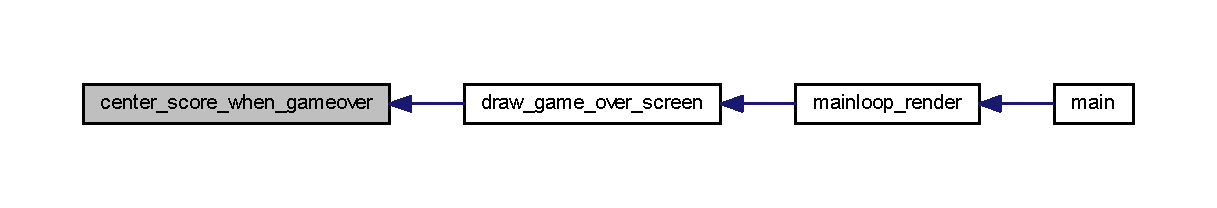
\includegraphics[width=350pt]{render_8c_aed4a93d083114e3b2160bc3adef848f5_icgraph}
\end{center}
\end{figure}
\hypertarget{render_8c_a9b14b8e82140fb3a218656d05ff72bc1}{}\label{render_8c_a9b14b8e82140fb3a218656d05ff72bc1} 
\index{render.\+c@{render.\+c}!draw\+\_\+game\+\_\+over\+\_\+screen@{draw\+\_\+game\+\_\+over\+\_\+screen}}
\index{draw\+\_\+game\+\_\+over\+\_\+screen@{draw\+\_\+game\+\_\+over\+\_\+screen}!render.\+c@{render.\+c}}
\subsubsection{\texorpdfstring{draw\+\_\+game\+\_\+over\+\_\+screen()}{draw\_game\_over\_screen()}}
{\footnotesize\ttfamily void draw\+\_\+game\+\_\+over\+\_\+screen (\begin{DoxyParamCaption}\item[{void}]{ }\end{DoxyParamCaption})}

This function draws the gameover screen.

\begin{DoxyAuthor}{Author}
Sebastian Dine 
\end{DoxyAuthor}
Here is the call graph for this function\+:\nopagebreak
\begin{figure}[H]
\begin{center}
\leavevmode
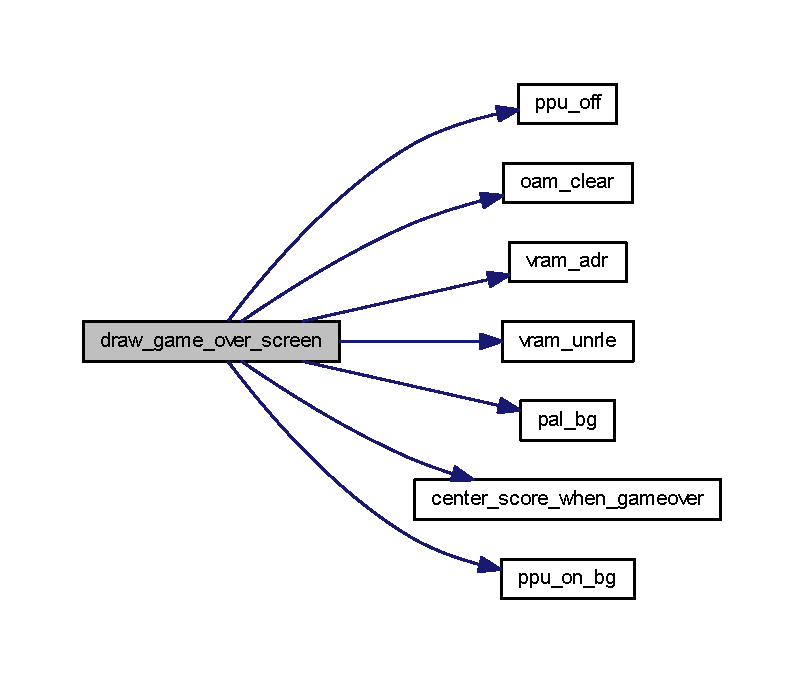
\includegraphics[width=350pt]{render_8c_a9b14b8e82140fb3a218656d05ff72bc1_cgraph}
\end{center}
\end{figure}
Here is the caller graph for this function\+:\nopagebreak
\begin{figure}[H]
\begin{center}
\leavevmode
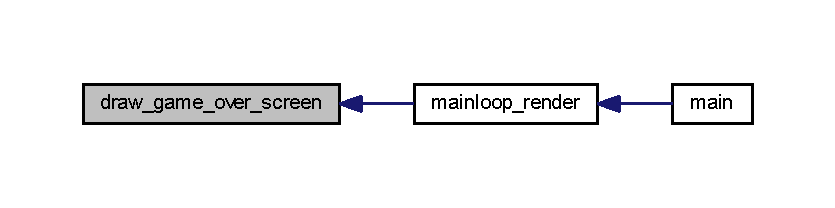
\includegraphics[width=350pt]{render_8c_a9b14b8e82140fb3a218656d05ff72bc1_icgraph}
\end{center}
\end{figure}
\hypertarget{render_8c_a2d33405474ba721e0d294333beb2db08}{}\label{render_8c_a2d33405474ba721e0d294333beb2db08} 
\index{render.\+c@{render.\+c}!draw\+\_\+item@{draw\+\_\+item}}
\index{draw\+\_\+item@{draw\+\_\+item}!render.\+c@{render.\+c}}
\subsubsection{\texorpdfstring{draw\+\_\+item()}{draw\_item()}}
{\footnotesize\ttfamily void draw\+\_\+item (\begin{DoxyParamCaption}\item[{void}]{ }\end{DoxyParamCaption})}

This function draws an element as a sprite to the screen.

\begin{DoxyAuthor}{Author}
Sebastian Dine 
\end{DoxyAuthor}
Here is the call graph for this function\+:\nopagebreak
\begin{figure}[H]
\begin{center}
\leavevmode
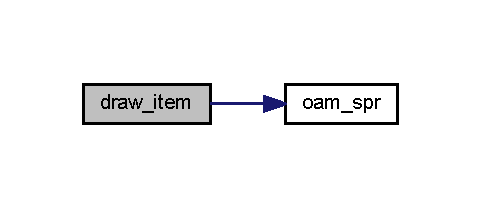
\includegraphics[width=231pt]{render_8c_a2d33405474ba721e0d294333beb2db08_cgraph}
\end{center}
\end{figure}
Here is the caller graph for this function\+:\nopagebreak
\begin{figure}[H]
\begin{center}
\leavevmode
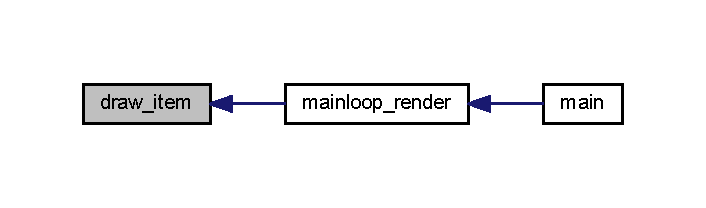
\includegraphics[width=339pt]{render_8c_a2d33405474ba721e0d294333beb2db08_icgraph}
\end{center}
\end{figure}
\hypertarget{render_8c_a0842d4314b6de6efca64c0ad01002712}{}\label{render_8c_a0842d4314b6de6efca64c0ad01002712} 
\index{render.\+c@{render.\+c}!draw\+\_\+level\+\_\+screen@{draw\+\_\+level\+\_\+screen}}
\index{draw\+\_\+level\+\_\+screen@{draw\+\_\+level\+\_\+screen}!render.\+c@{render.\+c}}
\subsubsection{\texorpdfstring{draw\+\_\+level\+\_\+screen()}{draw\_level\_screen()}}
{\footnotesize\ttfamily void draw\+\_\+level\+\_\+screen (\begin{DoxyParamCaption}\item[{void}]{ }\end{DoxyParamCaption})}

This function draws the background of the current level to the screen.

\begin{DoxyAuthor}{Author}
Sebastian Dine 
\end{DoxyAuthor}
Here is the call graph for this function\+:\nopagebreak
\begin{figure}[H]
\begin{center}
\leavevmode
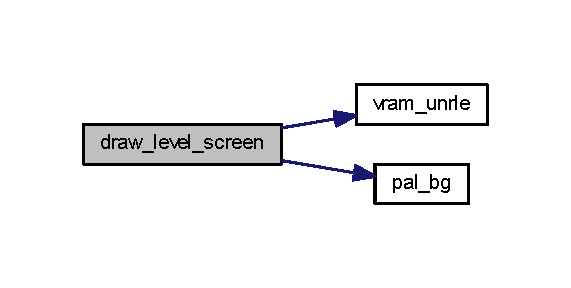
\includegraphics[width=274pt]{render_8c_a0842d4314b6de6efca64c0ad01002712_cgraph}
\end{center}
\end{figure}
Here is the caller graph for this function\+:\nopagebreak
\begin{figure}[H]
\begin{center}
\leavevmode
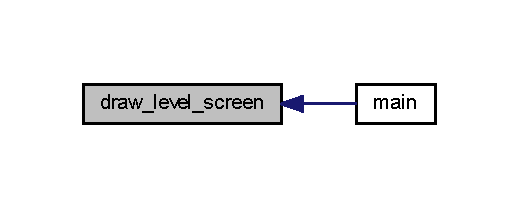
\includegraphics[width=249pt]{render_8c_a0842d4314b6de6efca64c0ad01002712_icgraph}
\end{center}
\end{figure}
\hypertarget{render_8c_ae7beeeddc3ba63a471ed7adf686d6751}{}\label{render_8c_ae7beeeddc3ba63a471ed7adf686d6751} 
\index{render.\+c@{render.\+c}!draw\+\_\+pause\+\_\+screen@{draw\+\_\+pause\+\_\+screen}}
\index{draw\+\_\+pause\+\_\+screen@{draw\+\_\+pause\+\_\+screen}!render.\+c@{render.\+c}}
\subsubsection{\texorpdfstring{draw\+\_\+pause\+\_\+screen()}{draw\_pause\_screen()}}
{\footnotesize\ttfamily void draw\+\_\+pause\+\_\+screen (\begin{DoxyParamCaption}\item[{void}]{ }\end{DoxyParamCaption})}

This function draws the letters P\+A\+U\+SE as sprites to the center of the screen, if the game is paused.

\begin{DoxyAuthor}{Author}
Sebastian Dine 
\end{DoxyAuthor}
Here is the call graph for this function\+:\nopagebreak
\begin{figure}[H]
\begin{center}
\leavevmode
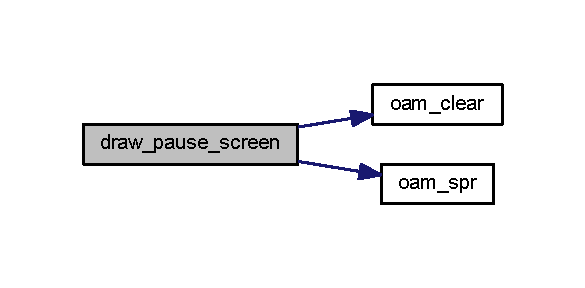
\includegraphics[width=281pt]{render_8c_ae7beeeddc3ba63a471ed7adf686d6751_cgraph}
\end{center}
\end{figure}
Here is the caller graph for this function\+:\nopagebreak
\begin{figure}[H]
\begin{center}
\leavevmode
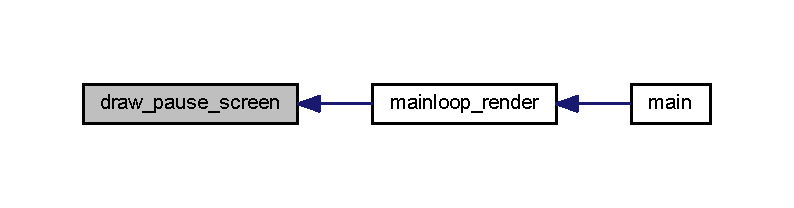
\includegraphics[width=350pt]{render_8c_ae7beeeddc3ba63a471ed7adf686d6751_icgraph}
\end{center}
\end{figure}
\hypertarget{render_8c_a38d38ff447a57a6f4406de8193e1a390}{}\label{render_8c_a38d38ff447a57a6f4406de8193e1a390} 
\index{render.\+c@{render.\+c}!draw\+\_\+score@{draw\+\_\+score}}
\index{draw\+\_\+score@{draw\+\_\+score}!render.\+c@{render.\+c}}
\subsubsection{\texorpdfstring{draw\+\_\+score()}{draw\_score()}}
{\footnotesize\ttfamily void draw\+\_\+score (\begin{DoxyParamCaption}\item[{void}]{ }\end{DoxyParamCaption})}

This function draws the current score as background tiles to the screen.

\begin{DoxyAuthor}{Author}
Sebastian Dine 
\end{DoxyAuthor}
Here is the caller graph for this function\+:\nopagebreak
\begin{figure}[H]
\begin{center}
\leavevmode
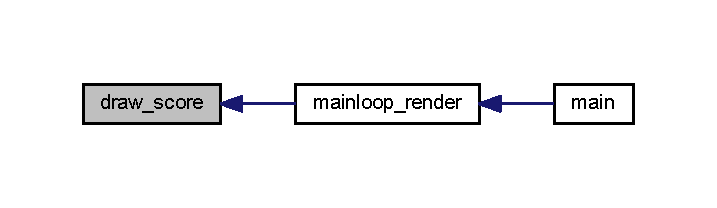
\includegraphics[width=344pt]{render_8c_a38d38ff447a57a6f4406de8193e1a390_icgraph}
\end{center}
\end{figure}
\hypertarget{render_8c_a115543b4c8b33eab539f43151ff51db3}{}\label{render_8c_a115543b4c8b33eab539f43151ff51db3} 
\index{render.\+c@{render.\+c}!draw\+\_\+snake@{draw\+\_\+snake}}
\index{draw\+\_\+snake@{draw\+\_\+snake}!render.\+c@{render.\+c}}
\subsubsection{\texorpdfstring{draw\+\_\+snake()}{draw\_snake()}}
{\footnotesize\ttfamily void draw\+\_\+snake (\begin{DoxyParamCaption}\item[{void}]{ }\end{DoxyParamCaption})}

This function draws the whole snake. The head will be drawn as a sprite, the body elements as background tiles.

\begin{DoxyAuthor}{Author}
Sebastian Dine 
\end{DoxyAuthor}
Here is the call graph for this function\+:\nopagebreak
\begin{figure}[H]
\begin{center}
\leavevmode
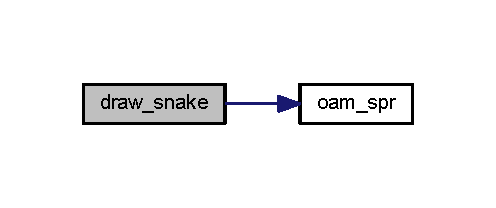
\includegraphics[width=238pt]{render_8c_a115543b4c8b33eab539f43151ff51db3_cgraph}
\end{center}
\end{figure}
Here is the caller graph for this function\+:\nopagebreak
\begin{figure}[H]
\begin{center}
\leavevmode
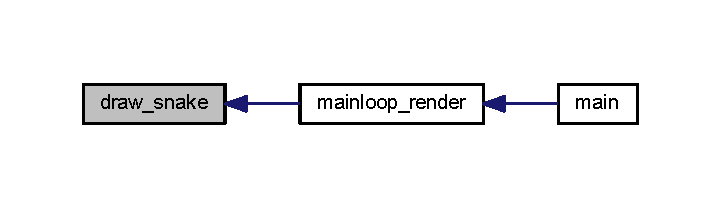
\includegraphics[width=346pt]{render_8c_a115543b4c8b33eab539f43151ff51db3_icgraph}
\end{center}
\end{figure}
\hypertarget{render_8c_a1b09050d2bea05fec0b30f6e452a2ff7}{}\label{render_8c_a1b09050d2bea05fec0b30f6e452a2ff7} 
\index{render.\+c@{render.\+c}!draw\+\_\+title\+\_\+screen@{draw\+\_\+title\+\_\+screen}}
\index{draw\+\_\+title\+\_\+screen@{draw\+\_\+title\+\_\+screen}!render.\+c@{render.\+c}}
\subsubsection{\texorpdfstring{draw\+\_\+title\+\_\+screen()}{draw\_title\_screen()}}
{\footnotesize\ttfamily void draw\+\_\+title\+\_\+screen (\begin{DoxyParamCaption}\item[{void}]{ }\end{DoxyParamCaption})}

This function draws the title screen.

\begin{DoxyAuthor}{Author}
Sebastian Dine 
\end{DoxyAuthor}
Here is the call graph for this function\+:\nopagebreak
\begin{figure}[H]
\begin{center}
\leavevmode
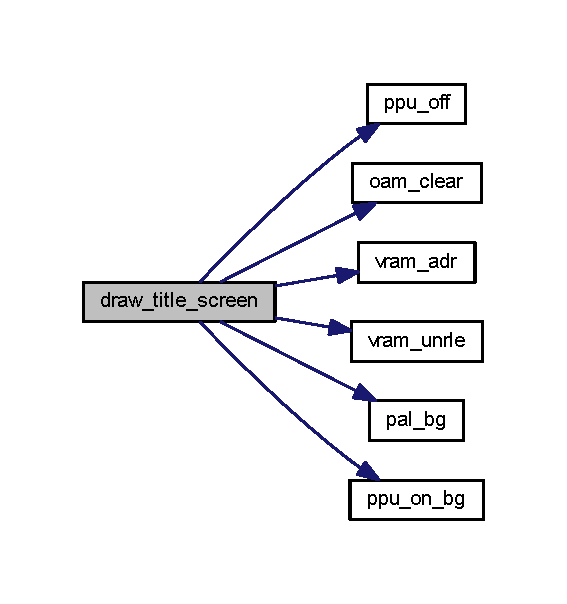
\includegraphics[width=272pt]{render_8c_a1b09050d2bea05fec0b30f6e452a2ff7_cgraph}
\end{center}
\end{figure}
Here is the caller graph for this function\+:\nopagebreak
\begin{figure}[H]
\begin{center}
\leavevmode
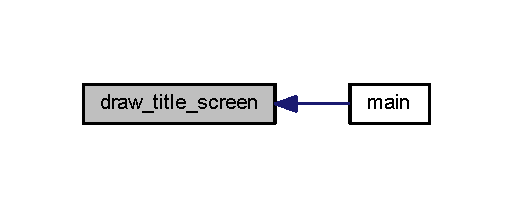
\includegraphics[width=246pt]{render_8c_a1b09050d2bea05fec0b30f6e452a2ff7_icgraph}
\end{center}
\end{figure}
\hypertarget{render_8c_aad91df7562212fbe50ec49e27ef5af3a}{}\label{render_8c_aad91df7562212fbe50ec49e27ef5af3a} 
\index{render.\+c@{render.\+c}!init\+\_\+update\+List@{init\+\_\+update\+List}}
\index{init\+\_\+update\+List@{init\+\_\+update\+List}!render.\+c@{render.\+c}}
\subsubsection{\texorpdfstring{init\+\_\+update\+List()}{init\_updateList()}}
{\footnotesize\ttfamily void init\+\_\+update\+List (\begin{DoxyParamCaption}\item[{void}]{ }\end{DoxyParamCaption})}

This function initializes the (background tile) update-\/list with score-\/elements (zero-\/digits) and the E\+O\+F-\/indicator.

\begin{DoxyAuthor}{Author}
Sebastian Dine 
\end{DoxyAuthor}
Here is the caller graph for this function\+:\nopagebreak
\begin{figure}[H]
\begin{center}
\leavevmode
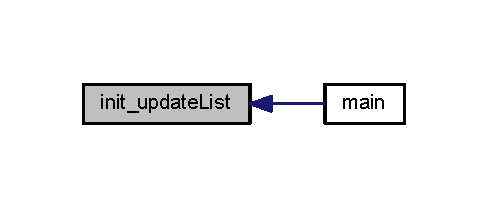
\includegraphics[width=234pt]{render_8c_aad91df7562212fbe50ec49e27ef5af3a_icgraph}
\end{center}
\end{figure}
\hypertarget{render_8c_aedd9dc656adabee0aaa1887fdc431544}{}\label{render_8c_aedd9dc656adabee0aaa1887fdc431544} 
\index{render.\+c@{render.\+c}!mainloop\+\_\+render@{mainloop\+\_\+render}}
\index{mainloop\+\_\+render@{mainloop\+\_\+render}!render.\+c@{render.\+c}}
\subsubsection{\texorpdfstring{mainloop\+\_\+render()}{mainloop\_render()}}
{\footnotesize\ttfamily void mainloop\+\_\+render (\begin{DoxyParamCaption}\item[{void}]{ }\end{DoxyParamCaption})}

This function provides the coordination of all render routines according to the current status of the game, once per frame.

\begin{DoxyAuthor}{Author}
Sebastian Dine 
\end{DoxyAuthor}
Here is the call graph for this function\+:\nopagebreak
\begin{figure}[H]
\begin{center}
\leavevmode
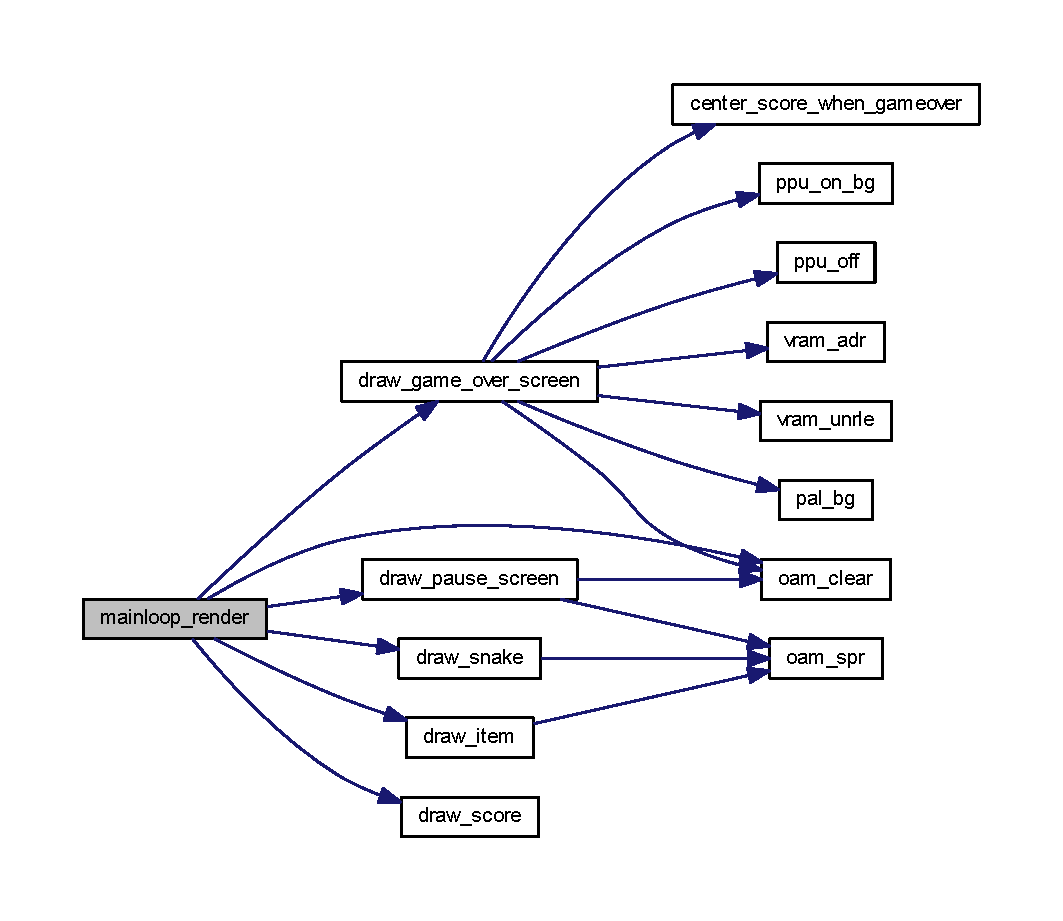
\includegraphics[width=350pt]{render_8c_aedd9dc656adabee0aaa1887fdc431544_cgraph}
\end{center}
\end{figure}
Here is the caller graph for this function\+:\nopagebreak
\begin{figure}[H]
\begin{center}
\leavevmode
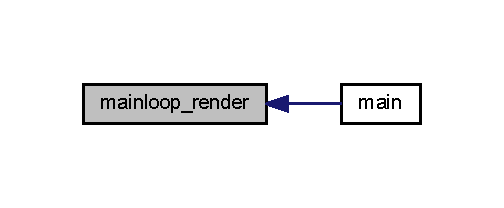
\includegraphics[width=242pt]{render_8c_aedd9dc656adabee0aaa1887fdc431544_icgraph}
\end{center}
\end{figure}

\hypertarget{snake_8c}{}\section{C\+:/\+Users/\+Administrator/\+Documents/\+Git\+Hub/\+N\+E\+S-\/\+Snake/src/snake.c File Reference}
\label{snake_8c}\index{C\+:/\+Users/\+Administrator/\+Documents/\+Git\+Hub/\+N\+E\+S-\/\+Snake/src/snake.\+c@{C\+:/\+Users/\+Administrator/\+Documents/\+Git\+Hub/\+N\+E\+S-\/\+Snake/src/snake.\+c}}


Maingame file, containing the main game loop.  


{\ttfamily \#include \char`\"{}level1\+\_\+nam.\+h\char`\"{}}\newline
{\ttfamily \#include \char`\"{}level2\+\_\+nam.\+h\char`\"{}}\newline
{\ttfamily \#include \char`\"{}game\+\_\+over\+\_\+nam.\+h\char`\"{}}\newline
{\ttfamily \#include \char`\"{}titlescreen\+\_\+nam.\+h\char`\"{}}\newline
{\ttfamily \#include \char`\"{}levels\+\_\+pal.\+h\char`\"{}}\newline
{\ttfamily \#include \char`\"{}sprites\+\_\+pal.\+h\char`\"{}}\newline
{\ttfamily \#include \char`\"{}menue\+\_\+pal.\+h\char`\"{}}\newline
{\ttfamily \#include \char`\"{}neslib.\+h\char`\"{}}\newline
{\ttfamily \#include \char`\"{}macros.\+h\char`\"{}}\newline
{\ttfamily \#include \char`\"{}structures.\+h\char`\"{}}\newline
{\ttfamily \#include \char`\"{}globals.\+h\char`\"{}}\newline
{\ttfamily \#include \char`\"{}init.\+c\char`\"{}}\newline
{\ttfamily \#include \char`\"{}input.\+c\char`\"{}}\newline
{\ttfamily \#include \char`\"{}update.\+c\char`\"{}}\newline
{\ttfamily \#include \char`\"{}render.\+c\char`\"{}}\newline
\subsection*{Functions}
\begin{DoxyCompactItemize}
\item 
void \hyperlink{snake_8c_a6288eba0f8e8ad3ab1544ad731eb7667}{main} (void)
\begin{DoxyCompactList}\small\item\em Main game loop. \end{DoxyCompactList}\end{DoxyCompactItemize}


\subsection{Detailed Description}
Maingame file, containing the main game loop. 

\begin{DoxyAuthor}{Author}
Sebastian Dine. 
\end{DoxyAuthor}


\subsection{Function Documentation}
\hypertarget{snake_8c_a6288eba0f8e8ad3ab1544ad731eb7667}{}\label{snake_8c_a6288eba0f8e8ad3ab1544ad731eb7667} 
\index{snake.\+c@{snake.\+c}!main@{main}}
\index{main@{main}!snake.\+c@{snake.\+c}}
\subsubsection{\texorpdfstring{main()}{main()}}
{\footnotesize\ttfamily void main (\begin{DoxyParamCaption}\item[{void}]{ }\end{DoxyParamCaption})}



Main game loop. 

\begin{DoxyAuthor}{Author}
Sebastian Dine 
\end{DoxyAuthor}
Here is the call graph for this function\+:\nopagebreak
\begin{figure}[H]
\begin{center}
\leavevmode
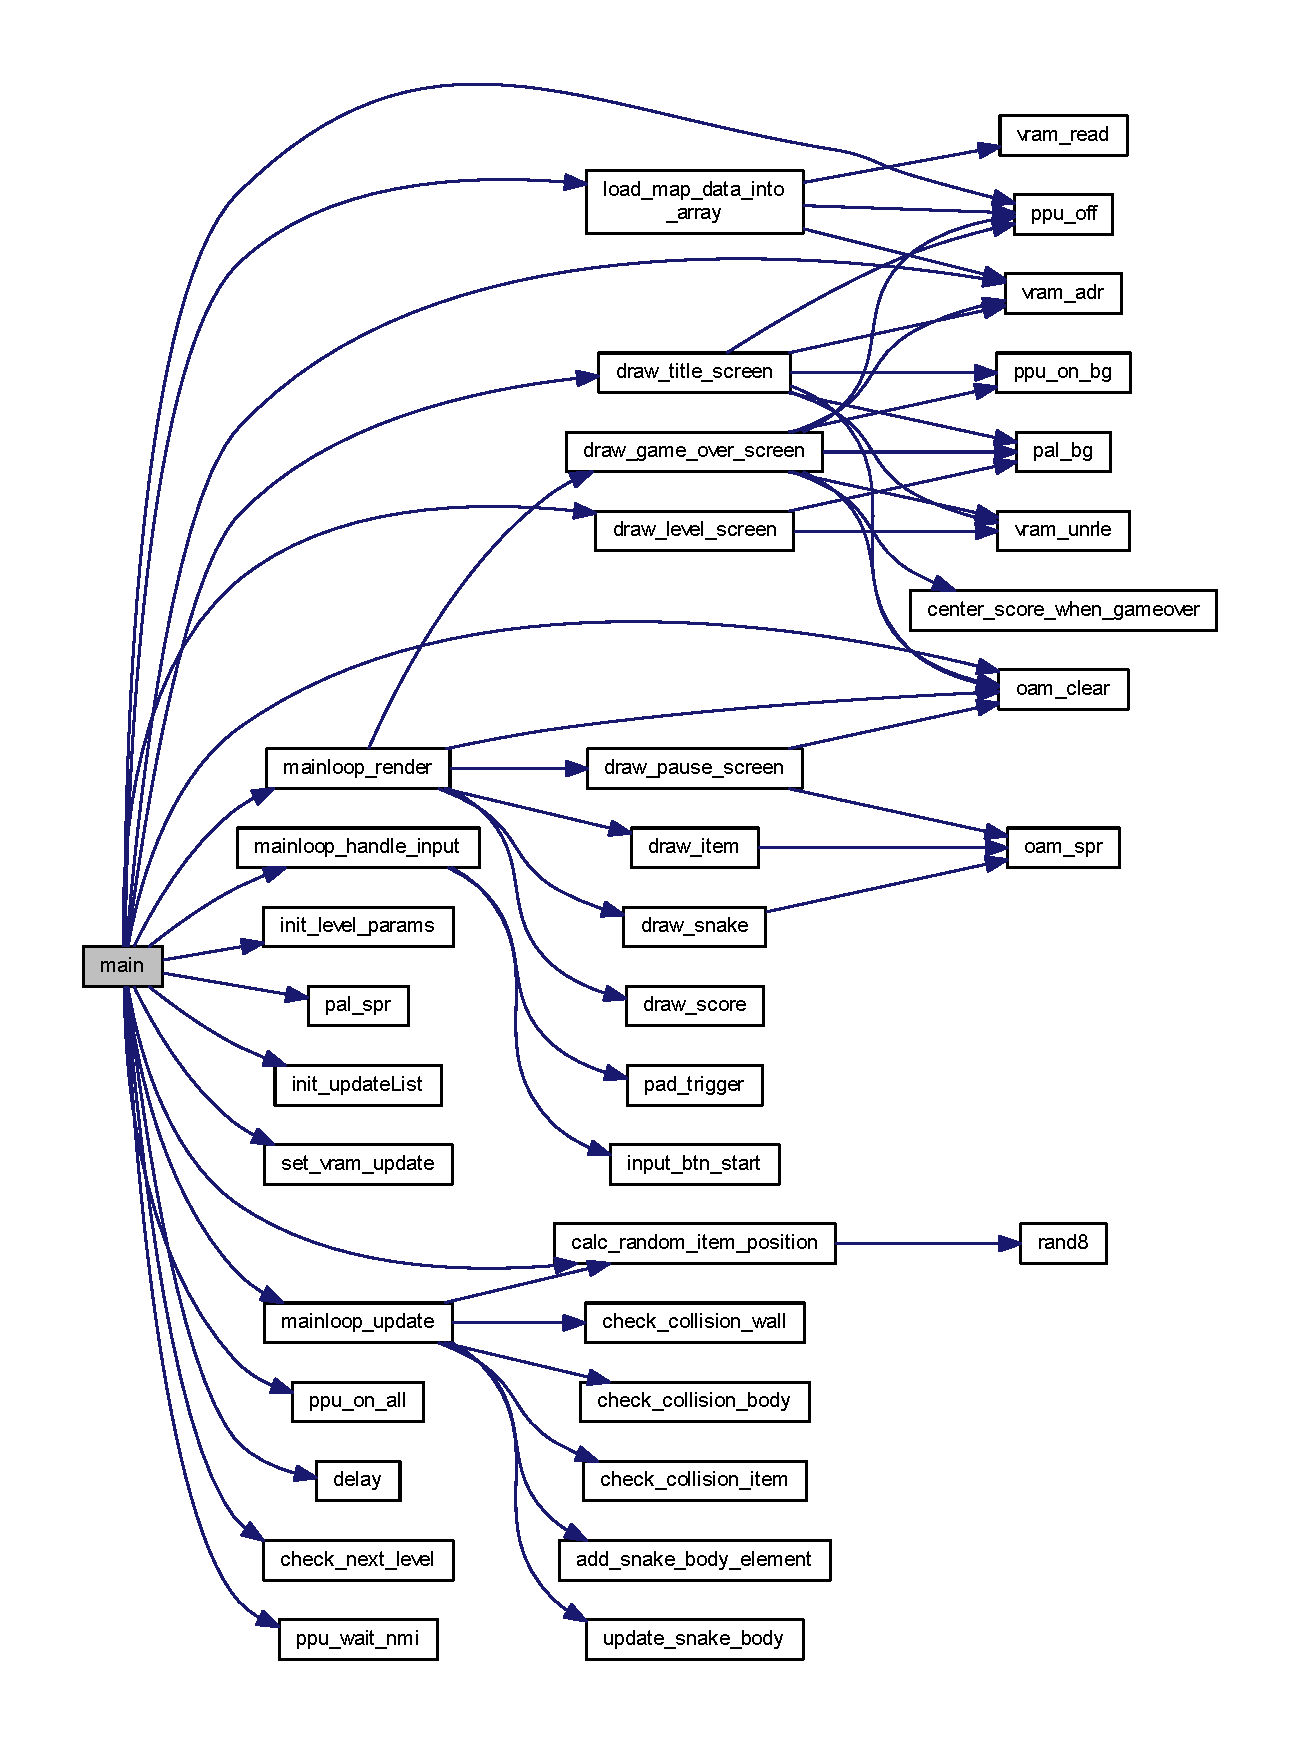
\includegraphics[height=550pt]{snake_8c_a6288eba0f8e8ad3ab1544ad731eb7667_cgraph}
\end{center}
\end{figure}

\hypertarget{structures_8h}{}\section{C\+:/\+Users/\+Administrator/\+Documents/\+Git\+Hub/\+N\+E\+S-\/\+Snake/src/structures.h File Reference}
\label{structures_8h}\index{C\+:/\+Users/\+Administrator/\+Documents/\+Git\+Hub/\+N\+E\+S-\/\+Snake/src/structures.\+h@{C\+:/\+Users/\+Administrator/\+Documents/\+Git\+Hub/\+N\+E\+S-\/\+Snake/src/structures.\+h}}


This header file contains the definition of structures, created for the purpose of the game.  


\subsection*{Data Structures}
\begin{DoxyCompactItemize}
\item 
struct \hyperlink{structsnake__struct}{snake\+\_\+struct}
\begin{DoxyCompactList}\small\item\em This structure contains all elements required to interact and display the snake. \end{DoxyCompactList}\end{DoxyCompactItemize}


\subsection{Detailed Description}
This header file contains the definition of structures, created for the purpose of the game. 

\begin{DoxyAuthor}{Author}
Sebastian Dine 
\end{DoxyAuthor}

\hypertarget{update_8c}{}\section{C\+:/\+Users/\+Administrator/\+Documents/\+Git\+Hub/\+N\+E\+S-\/\+Snake/src/update.c File Reference}
\label{update_8c}\index{C\+:/\+Users/\+Administrator/\+Documents/\+Git\+Hub/\+N\+E\+S-\/\+Snake/src/update.\+c@{C\+:/\+Users/\+Administrator/\+Documents/\+Git\+Hub/\+N\+E\+S-\/\+Snake/src/update.\+c}}


This file contains all ingame logic functionalities and utility functionalities.  


\subsection*{Functions}
\begin{DoxyCompactItemize}
\item 
void \hyperlink{update_8c_a5e1a11d04da8b93d988f7f469cced908}{calc\+\_\+random\+\_\+item\+\_\+position} (void)
\item 
void \hyperlink{update_8c_a9441f5df7c591a90d7cc8bda74209bef}{update\+\_\+snake\+\_\+body} ()
\item 
void \hyperlink{update_8c_ab8a45cae1f3c11e0ac4e758200257dd5}{add\+\_\+snake\+\_\+body\+\_\+element} ()
\item 
unsigned char \hyperlink{update_8c_a4a602dbc65a1829ae32ec9328241d016}{check\+\_\+collision\+\_\+wall} (void)
\item 
unsigned char \hyperlink{update_8c_a5fc00c88d57d8ba35a79d70316c2b478}{check\+\_\+collision\+\_\+body} (void)
\item 
unsigned char \hyperlink{update_8c_a10b8789c8aedb4abbcf3d3c98ed723e7}{check\+\_\+collision\+\_\+item} (void)
\item 
unsigned char \hyperlink{update_8c_a2ea36e0f75f408285b5d3a5bc8287b4f}{check\+\_\+next\+\_\+level} (void)
\item 
void \hyperlink{update_8c_a31c8504e7fe9671dbda52ba62a382b1f}{mainloop\+\_\+update} (void)
\end{DoxyCompactItemize}


\subsection{Detailed Description}
This file contains all ingame logic functionalities and utility functionalities. 

\begin{DoxyAuthor}{Author}
Sebastian Dine 
\end{DoxyAuthor}


\subsection{Function Documentation}
\hypertarget{update_8c_ab8a45cae1f3c11e0ac4e758200257dd5}{}\label{update_8c_ab8a45cae1f3c11e0ac4e758200257dd5} 
\index{update.\+c@{update.\+c}!add\+\_\+snake\+\_\+body\+\_\+element@{add\+\_\+snake\+\_\+body\+\_\+element}}
\index{add\+\_\+snake\+\_\+body\+\_\+element@{add\+\_\+snake\+\_\+body\+\_\+element}!update.\+c@{update.\+c}}
\subsubsection{\texorpdfstring{add\+\_\+snake\+\_\+body\+\_\+element()}{add\_snake\_body\_element()}}
{\footnotesize\ttfamily void add\+\_\+snake\+\_\+body\+\_\+element (\begin{DoxyParamCaption}{ }\end{DoxyParamCaption})}

This function adds a new pair of body element coordinates to global array \textquotesingle{}body\+\_\+coordinates\textquotesingle{}.

\begin{DoxyAuthor}{Author}
Sebastian Dine 
\end{DoxyAuthor}
Here is the caller graph for this function\+:\nopagebreak
\begin{figure}[H]
\begin{center}
\leavevmode
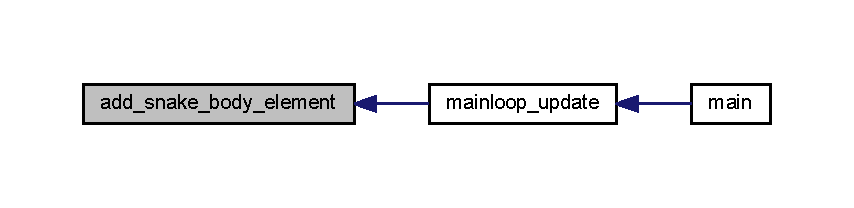
\includegraphics[width=350pt]{update_8c_ab8a45cae1f3c11e0ac4e758200257dd5_icgraph}
\end{center}
\end{figure}
\hypertarget{update_8c_a5e1a11d04da8b93d988f7f469cced908}{}\label{update_8c_a5e1a11d04da8b93d988f7f469cced908} 
\index{update.\+c@{update.\+c}!calc\+\_\+random\+\_\+item\+\_\+position@{calc\+\_\+random\+\_\+item\+\_\+position}}
\index{calc\+\_\+random\+\_\+item\+\_\+position@{calc\+\_\+random\+\_\+item\+\_\+position}!update.\+c@{update.\+c}}
\subsubsection{\texorpdfstring{calc\+\_\+random\+\_\+item\+\_\+position()}{calc\_random\_item\_position()}}
{\footnotesize\ttfamily void calc\+\_\+random\+\_\+item\+\_\+position (\begin{DoxyParamCaption}\item[{void}]{ }\end{DoxyParamCaption})}

This function calculates the coordinates of an grow-\/item. It stores the calculated coordinates into global fields \textquotesingle{}item\+\_\+x\textquotesingle{} and \textquotesingle{}item\+\_\+y\textquotesingle{}.

\begin{DoxyAuthor}{Author}
Sebastian Dine 
\end{DoxyAuthor}
Here is the call graph for this function\+:\nopagebreak
\begin{figure}[H]
\begin{center}
\leavevmode
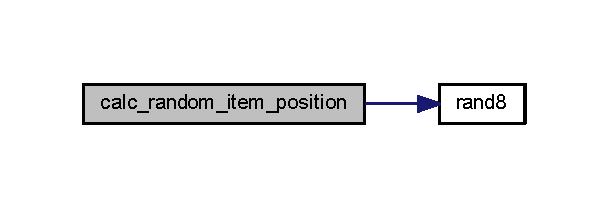
\includegraphics[width=292pt]{update_8c_a5e1a11d04da8b93d988f7f469cced908_cgraph}
\end{center}
\end{figure}
Here is the caller graph for this function\+:\nopagebreak
\begin{figure}[H]
\begin{center}
\leavevmode
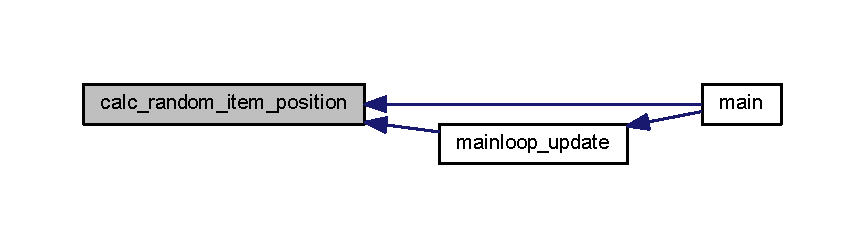
\includegraphics[width=350pt]{update_8c_a5e1a11d04da8b93d988f7f469cced908_icgraph}
\end{center}
\end{figure}
\hypertarget{update_8c_a5fc00c88d57d8ba35a79d70316c2b478}{}\label{update_8c_a5fc00c88d57d8ba35a79d70316c2b478} 
\index{update.\+c@{update.\+c}!check\+\_\+collision\+\_\+body@{check\+\_\+collision\+\_\+body}}
\index{check\+\_\+collision\+\_\+body@{check\+\_\+collision\+\_\+body}!update.\+c@{update.\+c}}
\subsubsection{\texorpdfstring{check\+\_\+collision\+\_\+body()}{check\_collision\_body()}}
{\footnotesize\ttfamily unsigned char check\+\_\+collision\+\_\+body (\begin{DoxyParamCaption}\item[{void}]{ }\end{DoxyParamCaption})}

Collision detecation of snakes\textquotesingle{} head-\/sprite with body-\/tiles.

\begin{DoxyReturn}{Returns}
1 = collision with body element, 0 = no collision with body element
\end{DoxyReturn}
\begin{DoxyAuthor}{Author}
Sebastian Dine 
\end{DoxyAuthor}
Here is the caller graph for this function\+:\nopagebreak
\begin{figure}[H]
\begin{center}
\leavevmode
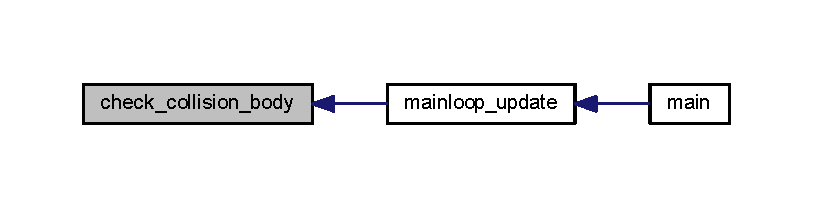
\includegraphics[width=350pt]{update_8c_a5fc00c88d57d8ba35a79d70316c2b478_icgraph}
\end{center}
\end{figure}
\hypertarget{update_8c_a10b8789c8aedb4abbcf3d3c98ed723e7}{}\label{update_8c_a10b8789c8aedb4abbcf3d3c98ed723e7} 
\index{update.\+c@{update.\+c}!check\+\_\+collision\+\_\+item@{check\+\_\+collision\+\_\+item}}
\index{check\+\_\+collision\+\_\+item@{check\+\_\+collision\+\_\+item}!update.\+c@{update.\+c}}
\subsubsection{\texorpdfstring{check\+\_\+collision\+\_\+item()}{check\_collision\_item()}}
{\footnotesize\ttfamily unsigned char check\+\_\+collision\+\_\+item (\begin{DoxyParamCaption}\item[{void}]{ }\end{DoxyParamCaption})}

Collision detection of snakes\textquotesingle{} head-\/sprite with an item-\/sprite.

\begin{DoxyReturn}{Returns}
1 = collision with item sprite, 0 = no collision with item sprite
\end{DoxyReturn}
\begin{DoxyAuthor}{Author}
Sebastian Dine 
\end{DoxyAuthor}
Here is the caller graph for this function\+:\nopagebreak
\begin{figure}[H]
\begin{center}
\leavevmode
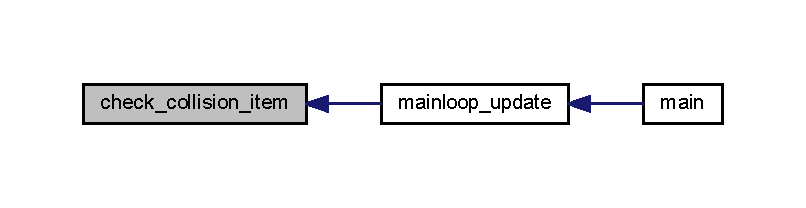
\includegraphics[width=350pt]{update_8c_a10b8789c8aedb4abbcf3d3c98ed723e7_icgraph}
\end{center}
\end{figure}
\hypertarget{update_8c_a4a602dbc65a1829ae32ec9328241d016}{}\label{update_8c_a4a602dbc65a1829ae32ec9328241d016} 
\index{update.\+c@{update.\+c}!check\+\_\+collision\+\_\+wall@{check\+\_\+collision\+\_\+wall}}
\index{check\+\_\+collision\+\_\+wall@{check\+\_\+collision\+\_\+wall}!update.\+c@{update.\+c}}
\subsubsection{\texorpdfstring{check\+\_\+collision\+\_\+wall()}{check\_collision\_wall()}}
{\footnotesize\ttfamily unsigned char check\+\_\+collision\+\_\+wall (\begin{DoxyParamCaption}\item[{void}]{ }\end{DoxyParamCaption})}

Collision detection of snakes\textquotesingle{} head-\/sprite with wall-\/tiles.

\begin{DoxyReturn}{Returns}
1 = collision with wall element, 0 = no collision with wall sprite
\end{DoxyReturn}
\begin{DoxyAuthor}{Author}
Sebastian Dine 
\end{DoxyAuthor}
Here is the caller graph for this function\+:\nopagebreak
\begin{figure}[H]
\begin{center}
\leavevmode
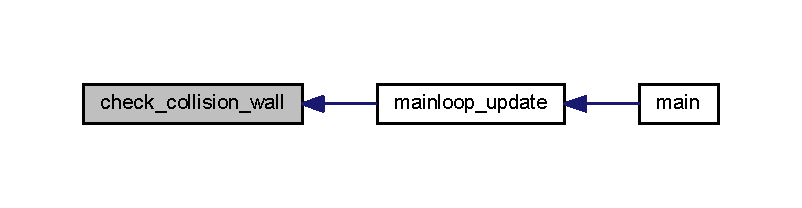
\includegraphics[width=350pt]{update_8c_a4a602dbc65a1829ae32ec9328241d016_icgraph}
\end{center}
\end{figure}
\hypertarget{update_8c_a2ea36e0f75f408285b5d3a5bc8287b4f}{}\label{update_8c_a2ea36e0f75f408285b5d3a5bc8287b4f} 
\index{update.\+c@{update.\+c}!check\+\_\+next\+\_\+level@{check\+\_\+next\+\_\+level}}
\index{check\+\_\+next\+\_\+level@{check\+\_\+next\+\_\+level}!update.\+c@{update.\+c}}
\subsubsection{\texorpdfstring{check\+\_\+next\+\_\+level()}{check\_next\_level()}}
{\footnotesize\ttfamily unsigned char check\+\_\+next\+\_\+level (\begin{DoxyParamCaption}\item[{void}]{ }\end{DoxyParamCaption})}

Check, if the requirements for the next level are met.

\begin{DoxyReturn}{Returns}
1 = next level is reached, 0 = next level is not reached
\end{DoxyReturn}
\begin{DoxyAuthor}{Author}
Sebastian Dine 
\end{DoxyAuthor}
Here is the caller graph for this function\+:\nopagebreak
\begin{figure}[H]
\begin{center}
\leavevmode
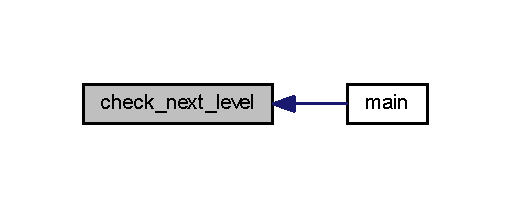
\includegraphics[width=245pt]{update_8c_a2ea36e0f75f408285b5d3a5bc8287b4f_icgraph}
\end{center}
\end{figure}
\hypertarget{update_8c_a31c8504e7fe9671dbda52ba62a382b1f}{}\label{update_8c_a31c8504e7fe9671dbda52ba62a382b1f} 
\index{update.\+c@{update.\+c}!mainloop\+\_\+update@{mainloop\+\_\+update}}
\index{mainloop\+\_\+update@{mainloop\+\_\+update}!update.\+c@{update.\+c}}
\subsubsection{\texorpdfstring{mainloop\+\_\+update()}{mainloop\_update()}}
{\footnotesize\ttfamily void mainloop\+\_\+update (\begin{DoxyParamCaption}\item[{void}]{ }\end{DoxyParamCaption})}

This function provides the coordination of all ingame logic routines, once per frame.

\begin{DoxyAuthor}{Author}
Sebastian Dine 
\end{DoxyAuthor}
Here is the call graph for this function\+:\nopagebreak
\begin{figure}[H]
\begin{center}
\leavevmode
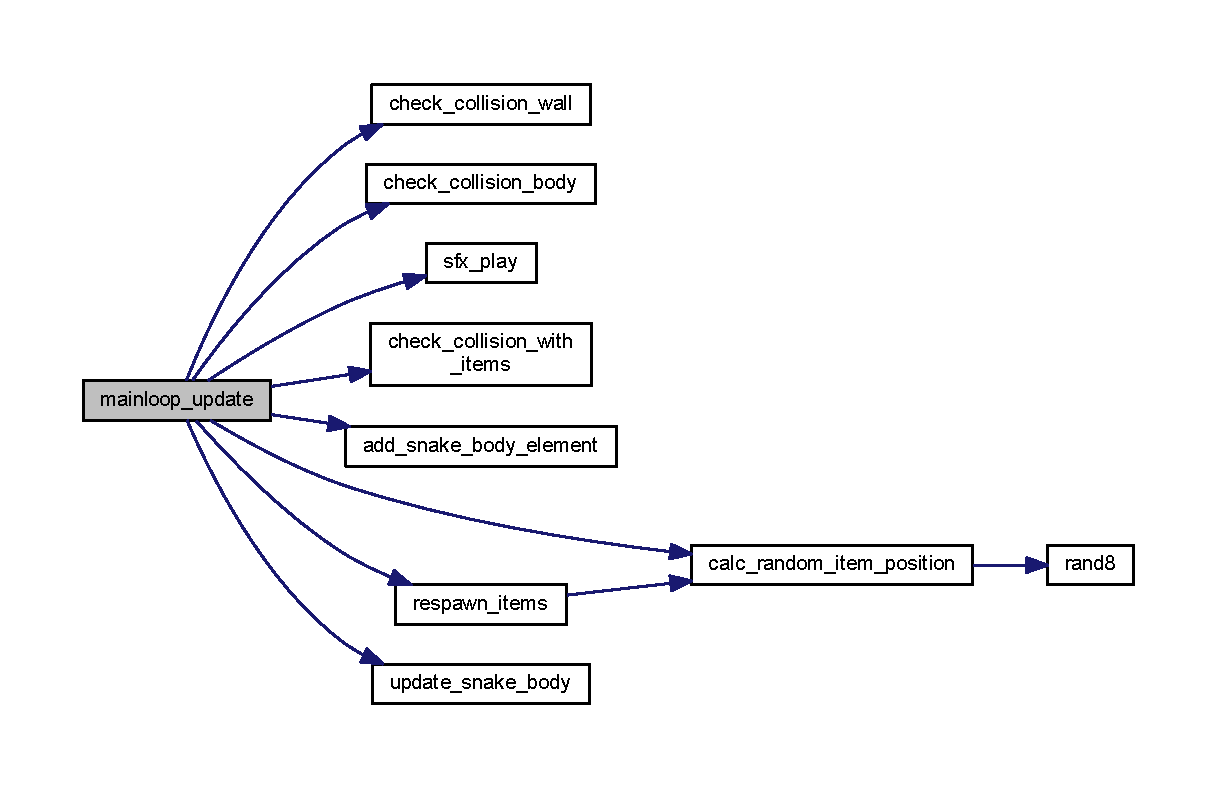
\includegraphics[width=350pt]{update_8c_a31c8504e7fe9671dbda52ba62a382b1f_cgraph}
\end{center}
\end{figure}
Here is the caller graph for this function\+:\nopagebreak
\begin{figure}[H]
\begin{center}
\leavevmode
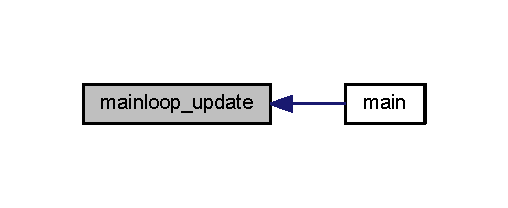
\includegraphics[width=244pt]{update_8c_a31c8504e7fe9671dbda52ba62a382b1f_icgraph}
\end{center}
\end{figure}
\hypertarget{update_8c_a9441f5df7c591a90d7cc8bda74209bef}{}\label{update_8c_a9441f5df7c591a90d7cc8bda74209bef} 
\index{update.\+c@{update.\+c}!update\+\_\+snake\+\_\+body@{update\+\_\+snake\+\_\+body}}
\index{update\+\_\+snake\+\_\+body@{update\+\_\+snake\+\_\+body}!update.\+c@{update.\+c}}
\subsubsection{\texorpdfstring{update\+\_\+snake\+\_\+body()}{update\_snake\_body()}}
{\footnotesize\ttfamily void update\+\_\+snake\+\_\+body (\begin{DoxyParamCaption}{ }\end{DoxyParamCaption})}

This function updates the body coordinates of the snake in order to simulate its movement.

\begin{DoxyAuthor}{Author}
Sebastian Dine 
\end{DoxyAuthor}
Here is the caller graph for this function\+:\nopagebreak
\begin{figure}[H]
\begin{center}
\leavevmode
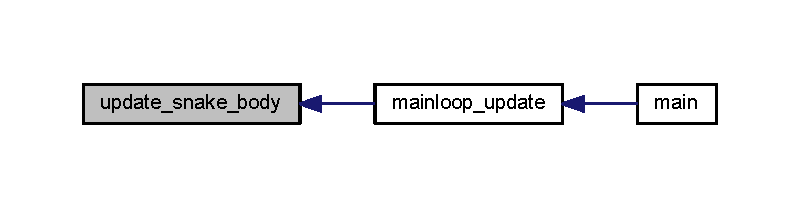
\includegraphics[width=350pt]{update_8c_a9441f5df7c591a90d7cc8bda74209bef_icgraph}
\end{center}
\end{figure}

%--- End generated contents ---

% Index
\backmatter
\newpage
\phantomsection
\clearemptydoublepage
\addcontentsline{toc}{chapter}{Index}
\printindex

\end{document}
